\documentclass[10pt,draftclsnofoot,onecolumn,retainorgcmds]{IEEEtran}
\usepackage[letterpaper, portrait, margin=0.75in]{geometry}
%\usepackage[myheadings]{fullpage}
\usepackage{fancyhdr}
\usepackage{lastpage}
\usepackage{graphicx, wrapfig, subcaption, setspace, booktabs}
\usepackage[T1]{fontenc}
\usepackage[font=small, labelfont=bf]{caption}
%\usepackage{fourier}
\usepackage[protrusion=true, expansion=true]{microtype}
\usepackage[english]{babel}
%\usepackage{sectsty}
\usepackage{url, lipsum}
\usepackage{tikz}
\usepackage{listings}
\usepackage{placeins}
\usepackage{enumitem}


\lstset{
	frame=single,
	breaklines=true,
	postbreak=\raisebox{0ex}[0ex][0ex]{\ensuremath{\color{red}\hookrightarrow\space}}
}

\newcommand{\namesigdatehrule}[1]{\par\tikz \draw [blue, densely dotted, ultra thick] (0,0) -- (#1,0);\par}
\newcommand{\namesigdate}[2][5cm]{%
\begin{minipage}{#1}%
    #2 \vspace{0.8cm}\namesigdatehrule{#1}\smallskip
    \small \noindent\textit{Signature}
    \vspace{0.8cm}\namesigdatehrule{#1}\smallskip
    \small \textit{Date}
\end{minipage}
}


\newcommand{\HRule}[1]{\rule{\linewidth}{#1}}
\newcommand*\tick{\textsc{\char13}}
\singlespacing
\setcounter{tocdepth}{5}
\setcounter{secnumdepth}{5}

\newcommand{\NHRule}{\rule{\linewidth}{0.5mm}} % Defines a new command for the horizontal lines, change thickness here

\begin{document}
%\title{HyRo}
%\author{Jason Klindtworth  |  Josh Asher  |   Layne Nolli}
%\date{}
%\maketitle
\begin{titlepage}
	\centering	
	\NHRule
	\vspace{1cm}
	{\scshape\LARGE HyRo \par}
	\vspace{1cm}
	{\scshape\Large Jason Klindtworth  |  Josh Asher  |   Layne Nolli\par}
	\vspace{1.5cm}
	\NHRule
	\vspace{1cm}
	{\huge\bfseries Capstone Team 28\par}
	\vspace{2cm}
	{\Large\itshape Final Report\par}
	\vspace{1cm}
	\vspace{1cm}
	{\large Abstract\par}
	\vspace{1cm}
	The project detailed in this document was developed over the course of the 2017 CS capstone class. It contains all our documentation, process, and reports surrounding our project. We had the awesome opportunity to be part of the Oregon State University hybrid rocket team. This was the first year a computer science team has been part of this team. The hybrid rocket is a cross disciplinary team consisting of mechanical engineers, electrical engineers, chemical engineers, and computer science engineers. We were tasked with developing the data visualization and control software for the team. Our software displays live sensor data while the rocket is in flight and records this data for later viewing. We also provide certain remote controls for operation of the rocket. \par
	\NHRule
	\vfill

% Bottom of the page
	{\large \today\par}
\end{titlepage}
\tableofcontents
\newpage

\section{Introduction}
\subsection{Oregon State Hybrid Program}
Here at Oregon State University there has been exciting momentum in the field of rocketry. A few years ago some student approached Dr. Nancy Squires about forming a rocket club. This evolved into being part of ESRA competition teams that compete nationally and has produced an on campus propulsion lab. We are proud to be sponsored by the AIAA in our endeavors. This program is very exciting for both students and teachers a like. It gives students a great chance to get started in aerospace. \par
About 2 years ago someone wanted to start a hybrid rocket team. A hybrid rocket is a rocket that used both solid and liquid fuel. Normally rocket use one or the other and the combustion material is mixed with the oxidizing material. In a hybrid rocket they are kept separately with the solid fill living in a tube that sits below a giant nitrous oxide injector. The hybrid rocket motors or more complex then your normal motor and take longer to design and build. They do have unique advantages over other types of rockets, for example they can be throttled. At OSU this program is still being developed and we are not part of any competitions yet, but the exiting part is that our work is leading towards getting into the competition. \par
The first year the hybrid rocket was a senior project they were not successful in getting the rocket off the ground. They did however build a nice launch rail. The second years team (last year) was successfully able to build and launch the rocket. With this success Dr. Squires, our client, wanted to bring more team members on from different parts of the University. So this year she built a team consisting of Mechanical, Electrical, Chemical, and Computer science engineers. This is a very important opportunity for students to experience real world situation were you will be working with many different types of engineers. Dr. Squires acts as the entire teams mentor, but allows the students to drive the project. This allowed us to be very creative while still having a supervisor to guide us through the process. \par
Each team took a different role in the project. The mechanical engineering team was divided into 4 sub teams each with about 3-4 members. These teams included structures, recovery/aerodynamics, hot end, and cold end. The structures team was responsible for the body design including the nose cone and all the support structure for the internal mounting of the sub systems. The recovery/aerodynamics team was responsible for the fin design and parachute system of the rocket. The cold end team was responsible for the pressurized tank, pluming, and injection system for the nitrous oxide, and the hot end team was responsible for the solid fuel combustion chamber and output of the rocket. The chemical engineering team was responsible for the solid fuel and testing different mixture to achieve an optimal burn. The electrical team was responsible for the avionics bay of the rocket. This includes all sensors, servos, parachute ejecting system, and radio communication to our software. \par
During this project we had to work closely with all the sub-teams in order to understand our requirements. We spent most of our time with the electrical team sense our sub systems worked with each other. This was a crucial part of our success and we had to learn to get along with and design with other teams in order to make the whole hybrid rocket project succeed. \par
\subsection{Our Project}
Dr. Squires came to us because the hybrid rocket was lacking a good way to visualize data and communicate commands. Prior years had only recorded data on a microcomputer but could not view it live. It dawned on her to open up this project to the CS capstone class in order to move the hybrid to the next step. It is important because we are trying to get into a competitions and she wanted the system to be complete in way similar to how the real rockets exists. Putting electronics and software in the rocket complicates the system, but allows for amazing things to occur. This is where we come in. \par
Our project was proposed to provide control buttons, data visualization, and logging for the team. We take the data provided by the Electrical team and display it on the screen through gauges and graphs. We also provide buttons to issue the rocket commands. This was essential since there is a great desire to operate certain aspects of the rocket from a distance. Each one of us took a different role to complete this project. Jason Klindtworth was in charge of graphical layout and design. He worked on making the interface look good and be functional. Layne Nolli took on the role of designing and implementing the drawing library and logging functions. Josh Asher was in charge of hardware interfacing, communication and data reception and queuing. We all took a role in combining this subcomponents in the main part of our program. \par
Our systems works like this: The on-board avionics system and our software establish a radio link through XBee radio transceivers. This is done through a serial API that is designed to work with the XBees. Our systems runs a thread that monitors for incoming radio transmissions. These transmissions contain a string of data that is then processed and put into data queues. As data comes into the queues another thread takes items from those queues and send them to drawing functions that graph the data on the screen. The screen is setup with 3 gauges (temperature, pressure, altitude) resembling gauges you would see on the dashboard of your car, then there are 5 graphs for acceleration, velocity, temperature, pressure, and altitude. Velocity is numerically derived. When data is draw it is also logged into time stamped folders where we collect the data to view later. A user can load data from any of the previous runs. To the left we provided buttons to issue remote commands to the rocket. When clicked a message is sent to the radio transceiver. \par
Our project was coded using python and its libraries. This language choice was made by the electrical engineers too. This made integration between our subsystems fairly easy. Python proved in the end to draw a little slow and we have had to make previsions before the launch to speed it up. Python was very simple to do the project in and amazed us through the project at how so few lines of code can do so much. \par


\begin{figure}[!ht]
	\caption{Screen shot of our final graphical user interface.}
	\centering
	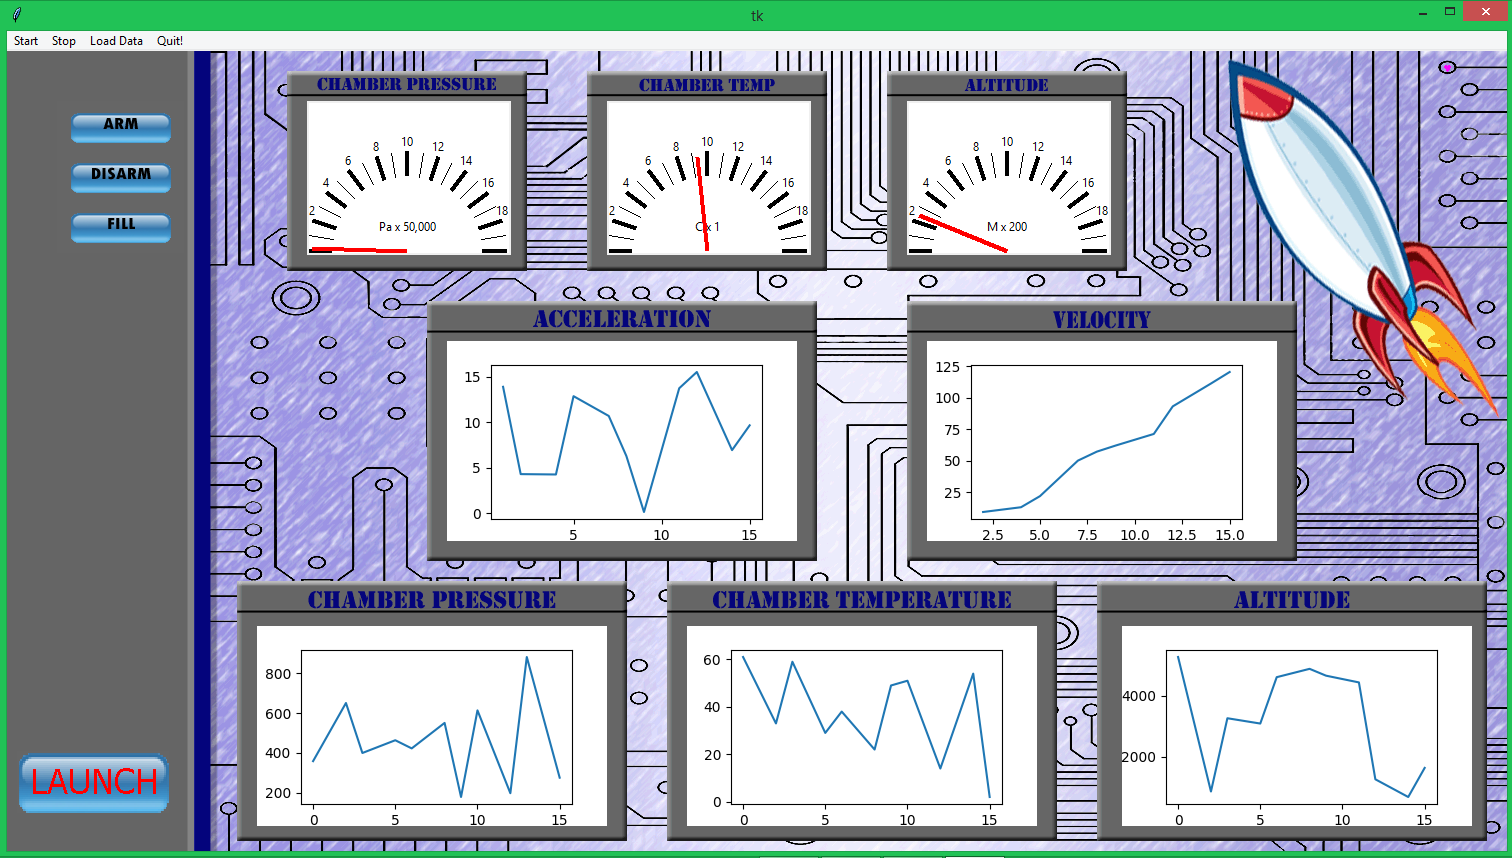
\includegraphics[scale=.45]{HyroGui}
\end{figure}

\section{Original Requirements Document and Subsequent Changes}
\begin{titlepage}
	\centering
	{\scshape\LARGE HyRo \par}
	%\vspace{1cm}
	{\scshape\LARGE Team 28\par}
	\vspace{1cm}
	{\scshape\Large Jason Klindtworth  |  Josh Asher  |   Layne Nolli}
	\noindent\makebox[\linewidth]{\rule{17cm}{2pt}}
	\vspace{1cm}
	{\huge\bfseries CS461\par}
	\vspace{2cm}
	{\Large\itshape Fall 2016\par}
	\vspace{4cm}
	{\large Requirements Document\par}\vspace{8cm}
	\noindent\makebox[\linewidth]{\rule{17cm}{2pt}}
	\vfill
	
	% Bottom of the page
	{\large \today\par}
\end{titlepage}

\section{ Introduction}
%\sectionfont{\scshape}
\subsection{Purpose}
\index{Purpose}
This document contains the software requirements that describe components of a system for a hybrid rocket that will communicate instructions, retrieve data, log commands,
visualize data, and visualize controls for such a rocket.  This document will provide scope, definitions, an overall description, and specific requirements for this system.
This system will be used by the OSU Hybrid Rocket team to launch and visualize data from their rocket. Persons involved include Nancy Squires, ME Senior Students, ECE senior students,
and other rocket club members that have chosen to be part of this team. Our audience members have an inclination to participate in rocketry. The system will be part of the ESRA
competition and has a potential to be recognized by the AIAA who support this competition.
\subsection{Scope}
\index{Scope}
There are 2 separate components to this avionics system. 

\subsubsection{HyRo OS}
\index{HyRo OS}
HyRo OS is a program residing on a Beagle Bone Black embedded Linux computer that will be onboard the hybrid rocket. This software component will collect sensor and possibly
GPS data from onboard electrical components and send this data to the ground team. HyRo OS is also responsible for receiving rocket commands from the ground team and responding to those
commands by sending electrical signals to appropriate onboard electrical equipment. The purpose of this component is to provide reliable communication to the ground team for commanding
the rocket and gathering its data. 
\subsubsection{HyRo VS}
\index{HyRo VS}
HyRo VS is software residing on a traditional computer that will send and receive data and commands to the rocket's onboard HyRo OS component. HyRo VS will be the ground teams graphical interface for data visualization, logging, and issuing commands to the system. It will present the ground team with input buttons to issue appropriate commands and data visualization windows to monitor data transferred from the hybrid rockets on board HyRo OS. This software will benefit the ground team by providing data visualization from the hybrid rocket that previously was not human readable. It also will provide command input into the system that benefits the ground team by ease of use and safety.

\subsection{Definitions, acronyms, and abbreviations}
\index{Definitions, acronyms, and abbreviations}
\subsubsection{\bf ESRA:}  The Experimental Sounding Rocket Association is a non-profit organization founded in 2003 for the purpose of fostering and promoting engineering in rocketry.
\subsubsection{\bf AIAA:} The American Institute of Aeronautics and Astronautics is the world's largest technical society dedicated to the global aerospace profession.
\subsubsection{\bf Avionics System:}  A system for controlling launch and other system function on a rocket, along with collecting data from onboard sensors.
\subsubsection{\bf Onboard:} Any component of the system that is housed in the rocket chassis.
\subsubsection{\bf Beagle Bone Black(BBB):}   A micro controller running Debian Linux connected to onboard components of the rocket.
\subsubsection{\bf HyRo OS:}  The HyRo rocket team's onboard operating system.
\subsubsection{\bf HyRo VS:} The HyRo rocket team's command and visualization software running on a traditional computer.
\subsubsection{\bf Embedded:} A software system that is running on microcontroller with no visual output.
\subsubsection{\bf Hybrid Rocket:} A rocket that has both solid fuel and liquid fuel. This creates the ability to throttle the rocket's motor.
\subsubsection{\bf GPS:} Global position satellite. In the aspect of this paper, a sensor that collects positional data in relation to the earth. This data is formatted for use in GPS applications to visualize the location of the sensor.
\subsubsection{\bf Ground Team:} The group of rocket team members controlling the rockets operation and viewing its data. Located a distance from the launch site on the ground.
\subsubsection{\bf Traditional Computer:}A computer, like a laptop, running an operating system. The operating system we will consider are Windows or Linux.
\subsubsection{\bf Remote Filling:} Filling the oxidizer from a safe distance via commands from the ground team.
\subsubsection{\bf Arming:} Preparing the rocket to ignite.
\subsubsection{\bf Disarming:} Reversing the rockets arming condition. 
\subsubsection{\bf Launch:} Releasing the rocket into the skies! 
\subsubsection{\bf Abort:} Completely stopping the rockets launching operations.
\subsubsection{\bf Ignition:} Starting the rocket motors combustion process.
\subsubsection{\bf Liquid Oxidizer:}Liquid part of the rockets fuel. 
\subsubsection{\bf Oxidizer Tank:} Tank were the liquid oxidizer is held. 
\subsubsection{\bf Chamber:} Where the two fuels mix.
\subsubsection{\bf PSI:}Pounds per square inch. A unit measuring pressure. 
\subsubsection{\bf Pa:} Pascals. A unit measuring pressure.
\subsubsection{\bf PWM:} Pulse Width Modulation - An electronic control signal used to change state of electrical components.
\subsubsection{\bf GPIO:}  General Purpose Input Output lines are used to communicate to sensors and electronic components.
\subsubsection{\bf SPI:}  Serial Peripheral Interface - A protocol to communicate with micro controllers.
\subsubsection{\bf I2C:}  Inter-Integrate Circuit - A protocol to communicate with micro controllers.
\subsubsection{\bf OS:} Operating System - the main system running on a micro controller or a traditional computer.
\subsubsection{\bf LSM9DS0:} The LSM9DS0 is a system-in-package featuring a 3D digital linear acceleration sensor,  a 3D digital angular rate sensor, and a 3D digital magnetic sensor.
\subsubsection{\bf TGY6114MD:}A powerful high specification digital sail winch servo with metal gears that can be programmed to operate from 1 to 6 turns.
\subsubsection{\bf BM180:}Digital pressure sensor.
\subsubsection{\bf API:}An application program interface is a set of routines, protocols, and tools for building software applications. An API specifies how software components should interact.
\subsubsection{\bf RAM:}Random Access Memory
\subsubsection{\bf Gauge:}A graphical device to display the readout of a sensor. For example a speedometer.
\subsubsection{\bf Serial Communication:}Data sent back to back through a medium.

\subsection{ References}
Beagle Bone Black hardware specifications from elinux.org [http://elinux.org/Beagleboard:BeagleBoneBlack]\\
BMP180 Digital Pressure Sensor data sheet [https://cdn-shop.adafruit.com/datasheets/BST-BMP180-DS000-09.pdf]\\
LSM9DS0 3D accelerometer, 3D gyroscope, 3D magnetometer data sheet http://www.st.com/content/ccc/resource/technica\\l/document/datasheet/ab/2a/3b/45/f0/92/41/73/DM00087365.pdf/files/DM00087365.pdf/jcr:content/translations\\/en.DM00087365.pdf]
\index{References}
\subsection{Overview}
\index{Overview}
The rest of this document contains over all descriptions of the different components of this system. Followed by specific requirements of these components.

\section{ Overall Description}
\index{Overall Description}
\subsection{ Product perspective}
\index{Product perspective}
Our software components are part of the overall system of the Hybrid Rocket. These components encompass remotely filling, arming/disarming, aborting, ignition, recovery, throttling, gathering sensor data, and radio communication circuitry.  On the traditional computer they encompass serial communication to the ground control unit, user input, and user data visualization. Our software will need to interface with an external GPS system if this stretch goal is reached. 

\subsubsection{System Interfaces}
\index{System Interfaces}
The HyRo VS component of our system will house the user interface to our system. This interface will be divided into a command menu, system diagnostics/status window, and different visualization windows with options on how to display the data. The full graphical user interface will fill the entire screen. The command menu will house six buttons with the potential for more to be added if necessary. All commands have not been decided on because the rocket has yet to be made and requirements and commands may be presented to our system as other teams design their parts of the hybrid rocket.  The six buttons that are required at the moment are: Arm Rocket, Disarm Rocket, Fill Liquid Oxidizer, Launch, Abort Launch, and Ignition. The command menu will be located to the left of the screen and take up approximately 1/4 the width of the screen and approximately 1/2 the height of the screen. Buttons in the menu will be evenly spaced and use around a size 20pt font for text inside the buttons. \par
Under the command menu on the left hand side of the screen will be the system diagnostics and status window. This window will take up 1/4 the width of the screen and 1/4 the height of the screen. This screen will report status of the various system components including indication of functioning communication between the hybrid rocket, the ground control unit, and the system which this software resides on. It will also include the state of the rocket (i.e. armed, disarmed, filled, etc) and any diagnostic information from sensors on the various components of the system. Exact diagnostic items have not been determined because the Hybrid Rocket has not been mechanically or electrically designed yet. These will be added to this document when the system is further along.\par 
Under the status window will be a graphing window options menu. This will take up 1/4 the width of the screen on the left and 1/4 its height. From this menu a user can select if they would like to individually look at larger graph of a particular piece of data. \par
The visualization windows will be housed in a parent container that will encompass 3/4 of the screen width and the total height of the screen. There is a total of 7 different groups of data that need to be visualized.  If any more sensors are added to this system once it is developing these will be added to this document with and explanation as to how they will be visualized.  The current group of data to be visualized includes:  Oxidizer tank pressure, chamber pressure, Oxidizer tank temperature, acceleration, barometric pressure, velocity, and GPS.   Each individual item might be represented as a gauge or graph.\par

The visualization units have not fully been determined and are listed as options until further development of the hybrid rocket occurs and we have feedback from the rest of the team as to what units will be the most appealing. Users will have the option to either graph the data or display the data in gauge format with a needle pointing to the current value of that data. \par


\begin{figure}
	\caption{Basic Mock Up of User Interface for Hyro showing implementation of UI layout and positioning of objects like buttons, graphs, and dials for the user to process at a glance. This is a test mock up and may not be exact to the final product. }
	\centering
	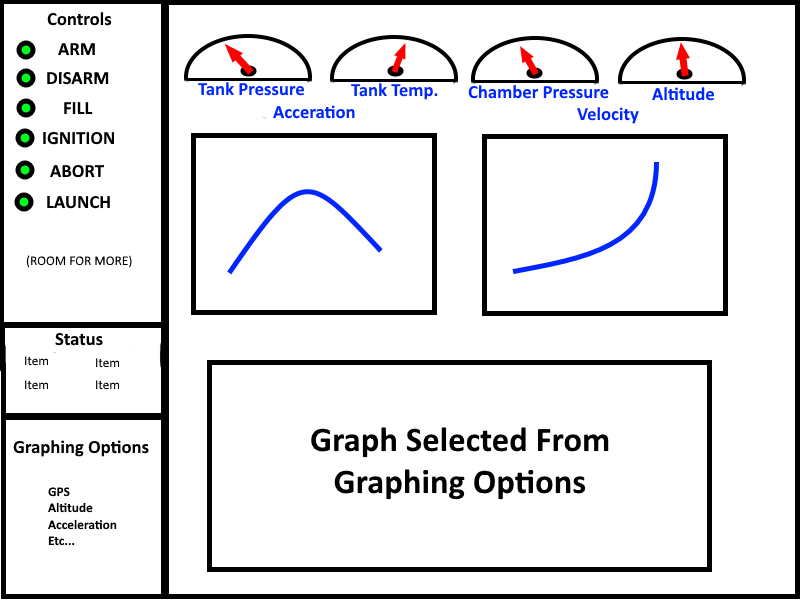
\includegraphics[scale=.75]{HyRoUIMockup}
\end{figure}
\index{User Interface Mockup}
\FloatBarrier
\subsubsection{Hardware Interfaces}
\index{Hardware Interfaces}
Each of the three components to our software will require specific interfaces to different hardware aspects depending on which part of the system they are located in.\par

{\bf HyRo OS}
HyRo OS will be connected to the onboard electrical systems of the rocket. These systems include sensors that collect data, servos that control various action internal to the rocket, a radio frequency transmitter for communication, and any other electrical device critical to the rockets operation. Many of these components have yet to be determined and will be conceived next term when work begins on the mechanical and electrical aspects of the rocket.  We do know all sensors on board the rocket from last year have pre-built interfaces that can connect to the BBB using common electrical protocols like I2C or SPI. They come with an API that can be used on the BBB to access their data. . Servos and other electrical components will use PWM lines available on the BBB to communicate desired functionality. The radio module used communicates to the BBB via serial communication. All the GPIO, PWM, and Serial lines on the BBB are interfaced through its operating system and come pre-configured for API access.\par

{\bf HyRo VS}
HyRo VS will need to communicate to a serial port on the computer it is residing on.  This will be done through either a Windows or Linux serial port access API.

\subsubsection{Software Interfaces}
\index{Software Interfaces}
We will be interfacing various outside software products. These include the Debian Linux operating system running on the BBB, the Operating system running on the traditional computer which will be either Linux or Windows and possibly an external GPS program which is part of our stretch requirements.

\subsubsection{Communication Interfaces}
\index{Communication Interfaces}
There are two interfaces for communication in our system and both require the use of a serial interface. The first is radio communication with a radio frequency transceiver. There will be one onboard the rocket connected to the BBB and one connected to the traditional computer via a USB interface. The serial communication is accessed through an API and acts like a file descriptor. We will design a protocol to transfer commands and data over these serial interfaces. Each command will have a name and parameters associated with it. Data will have a name associated with it followed by the actual data.

\subsubsection{Memory Constraints}
\index{Memory Constraints}
The HyRo VS aspect of our system will be constrained by the memory of the traditional computer it is located on. Available memory should be significant enough that we should not be constrained. This is because our program will have a small footprint and the data we log will not exceed 200 megabytes.\par 
The HyRo OS will be constrained to 512 megabytes of RAM and 4 Gigabytes of onboard long term memory. Our onboard system will need to be able to run in the RAM available and not store over 4 gigabytes of data.


\subsubsection {Operations}
\index{Operations}
There are 4 modes of operation in our system: pre-launch, staging, in flight, and post flight.  Pre-launch operations will be non-interactive and display status of the system components. The system will process data relating to the status of onboard components and display them in the status window. All buttons will be highlighted in a color corresponding to their status. We will have a background system monitoring all input from the control mechanism sent through the serial communication. \par
Staging will be an interactive process where the user will provide input to various command buttons. The buttons will have to be executed in order, except for the abort button. Components will monitor user input and prime the ignition system as defined by the ignition sequence. These functions will not allow user input in the wrong order. If the abort command is issued all other function will be overridden and the system will return to its pre-launch state. Once the sequence has been completed the software will switch to the in-flight mode. A support function that logs all commands to a log file will be implemented to record these actions.\par
The in-flight mode will disable the command menu and begin data collection from the onboard sensors. At this point all sensor data processing function will be activated. The data will be received from the serial port, parsed through the data processor, and sent to the appropriate data processing functions. These functions are responsible for visualizing the data on our graphs and gauges. These operations are to be monitored by the user for visual satisfaction.  The data will also be logged by a logging function in a text format to be used by the post-flight mode.
Post flight mode will be fully interactive. The command menu will still be disabled but data stored by the data logger will be able to be viewed in graphs that related the data over time of flight. These graphs will be viewable by selecting them from the data menu and expressing which data items you would like to see a graph of. \par

\subsubsection{Site Adaption Requirements}
\index{Site Adaption Requirements}
When the hybrid rocket is ready to launch the software will be in pre-launch mode and a sequence of commands must be sent to the rocket in order for the rocket to be safely launched. This sequence is fill, arm, ignite, and launch. At any moment someone can cancel this sequence if the rocket is deemed not safe to launch by using the abort button.

\subsection{ Product functions}
\index{Product functions}
Our software as a whole will function as a way to communicate information from the hybrid rocket to a traditional computer on the ground. The ground team will interact with the ground computer to look at the information from the rocket and pass information back to the rocket. Both software components each have their own unique functions.

\subsubsection{HyRo OS}
\begin{itemize}
	\item Send and Receive communications from a radio transceiver to communicate with the ground team.
	\item Collect sensor data from any onboard sensors when in flight.
	\item Send sensor data to the ground computer.
	\item Monitor fill and launch systems and send information to ground team.
	\item Receive commands from ground team.
	\item Send electrical signals or messages to launching components when appropriate command is received.
	\item Make sure commands are executed in correct order.
	\item Send signal to deploy chute at correct altitude.
\end{itemize}

\subsubsection{HyRo VS}
\begin{itemize}
	\item Send and Receive communication from a radio transceiver to communicate with the hybrid rocket.
	\item Provide a status view so team can monitor onboard rocket components.
	\item Provide a menu of commands to stage, launch, or abort the rocket mission.
	\item Log all commands that have been sent.
	\item Collect data sent from the rocket and store it.
	\item Collect data from the rocket and visualize it on the screen in its appropriate gauge or graph while rocket is in flight.
	\item Provide a log of the data.
	\item Provide the ability to view different categories of data in a graph with a menu for the user to choose what data from the flight they would like to view.\end{itemize}

\begin{figure}[!ht]
	\index{Data Flow Diagram of HyRo}
	\caption{Data Flow Between System Components.}
	\centering
	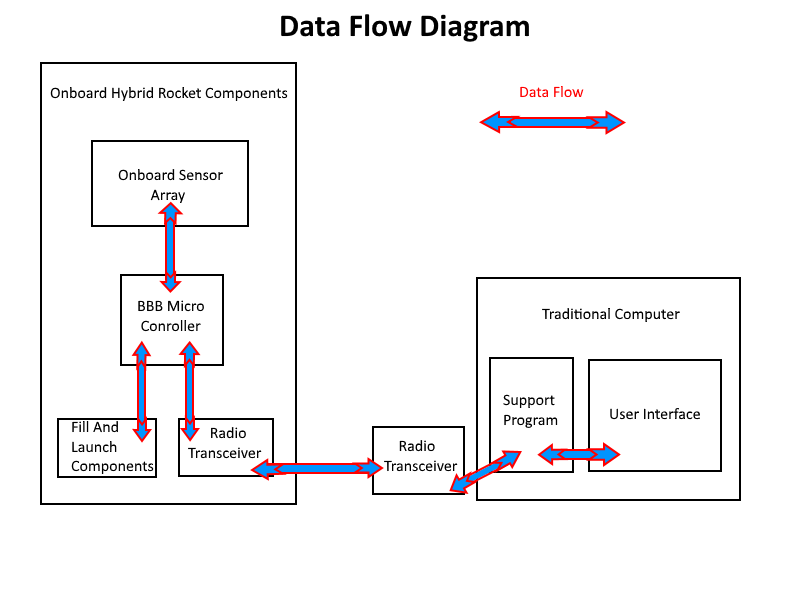
\includegraphics[scale=.85]{RocketBlockDiagram}
\end{figure}
\FloatBarrier
\subsection{ User characteristics}
\index{User characteristisc}
Intended users of this software require a knowledge of rocketry and safe handling of launching a rocket. These users will be undergraduate students, graduate students, and professors included in the rocket team. They will have sufficient knowledge of the operation and safety requirements of launching a hybrid rocket according to the safety regulation of ESRA.

\subsection{Constraints}
\index{Constraints}

\index{Regulatory Policies}
\subsubsection{\bf  Regulatory Policies}Operation of our software must stay in the bounds set by ESRA and the safe handling and operation of launching a hybrid rocket.  

\index{Hardware Limitations}
\subsubsection{\bf Hardware Limitations} HyRo OS will be onboard a BBB with only 512 megabytes of ram and 4 gigabytes of storage and must function under these restrictions. The BBB will also be inside of a volatile environment inside the rocket that could cause it to overheat. Timing is also a major concern in communicating sensor data and commands. All communication between the rocket, its sensors, its launching components, and the ground team must be within 1  second or less.

\index{Interfaces to other applications}
\subsubsection{\bf  Interfaces to other applications} If GPS is used we will have to output data to a GPS application in the correct format for that application.
\index{Control Functions}
\subsubsection{\bf Control Functions} Launching of the rocket must be monitored in the correct order or our software should not continue the sequence to launch the rocket.
\index{Reliability Requirements}
\subsubsection{\bf Reliability Requirements} Data in our system must be transferred and interpreted in a complete and reliable fashion. Incomplete commands will be ignored. Incomplete sensor data will also be ignored. Data loss will not exceed 10 percent or our system will not be reliable.
\index{Safety Considerations}
\subsubsection{\bf Safety Considerations} Our software must not stage and launch the rocket without receiving the appropriate sequence of commands from the ground team. Failure to do so may result in harm to team members.

\subsection{Assumptions and dependencies}
\index{Assumptions and dependencies}
Our onboard software system HyRo OS assumes that it will be installed on a Debian Linux OS that is running on a BBB.  HyRo OS assumes it will be connect to a XBee radio transceiver, a TGY6114MD servo, a LSM9DS0 accelerometer/gyroscope, and a BMP180 Barometric pressure altitude sensor.\par
Our HyRo VS software running on a traditional computer assumes that it will be communicating with a XBee radio transceiver.

\subsection{Apportioning of Requirements}
\index{Gantt Chart for HyRo}
\begin{figure}
	\caption{Gantt chart for HyRo Workflow over the course of the project. This chart is highlighting overlapping responsibilities between team members that are broken into manageable chunks to ensure time management. }
	\centering
	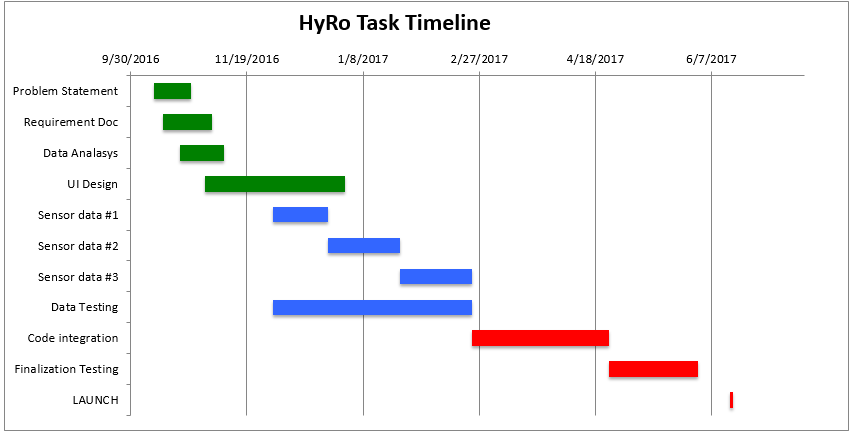
\includegraphics[scale=.75]{GanntChart}
\end{figure}
\FloatBarrier
\subsubsection{\bf GPS - (Stretch Goal)} A GPS sensor might be installed on the rocket. This will require the HyRo OS to be able to communicate with this sensor and transmit its data. The HyRo VS then will need to be able to collect this data and either display it in a GPS window of our design or pass it onto to a GPS application that will interpret the data to find the rockets location.
\subsubsection{\bf Throttling - (Stretch Goal)} If the system is stable in time the team would like to be able to automatically throttle the rocket in flight. Throttling will enable the rocket to reach a higher altitude. The HyRo OS will need to make inflight calculations and adjust the Oxidizer valve to the appropriate throttling level. This will require advanced math calculations and accurate valve adjusting.

\section{ Specific requirements}
\subsection{External Interface Requirements}
\index{User Interface Requirements}
\subsubsection{ User Interfaces}
\index{User Interfaces}
\paragraph {\bf Fill Command Button Input}
\index{Fill Command}
The fill command input button will activate the fill servo to fill the chamber with oxidizer. This command is inputted from a button on the command menu. The command will be formatted in an English representation.  This command must be sent within 1 second. This command must be sent before the arming command is given. Other commands will not function out of this sequence. It will be located in the command menu of the left hand side of the screen.

\paragraph{\bf Arming Command Button Input}
\index{Arming Command}
The arming command input button will send a command to the system that will arm the rocket. This command is inputted from a button on the command menu. The command will be formatted in an English representation.  This command must be sent within 1 second. This command must be sent before the ignition command is given. Other commands will not function out of this sequence. It will be located in the command menu of the left hand side of the screen.

\paragraph{\bf Ignition Command Button Input}
\index{Ignition Command}
The ignition command input button will activate the ignition system of the rocket. This command is inputted from a button on the command menu. The command will be formatted in an English representation.  This command must be sent within 1 seconds. This command must be sent before the launch command is given. Other commands will not function out of this sequence. It will be located in the command menu of the left hand side of the screen.

\paragraph{\bf Launch Command Button Input}
\index{Launch Command}
The launch command input button will release the rocket when it is ignited. This command is inputted from a button on the command menu. The command will be formatted in an English representation.  This command must be sent within 1 second. This command must be sent last in the sequence of commands. Other commands will not function out of this sequence. It will be located in the command menu of the left hand side of the screen.

\paragraph{\bf Disarm Command Button Input}
\index{Disarm Command}
The disarm command input button will disable the arming of the rocket. This command is inputted from a button on the command menu. The command will be formatted in an English representation.  This command must be sent within 1 second. This command can be issued anytime the rocket has been armed. It will be located in the command menu of the left hand side of the screen.

\paragraph{\bf Abort Command Button Input}
\index{Abort Command}
The abort command input button will return the system to its pre-launch state and stop the rocket from launching. This command is inputted from a button on the command menu. The command will be formatted in an English representation.  This command must be sent within 1 second. This command can be issued at any time and is not effected by other command buttons. It will be located in the command menu of the left hand side of the screen.

\paragraph{\bf Command Output to radio transceiver}
\index{Command Output}
Any time a command is received from the command menu the HyRo VS will send the command to the radio transceiver. The UI for the commands will all be formatted in plain English. Commands must be delivered in under 1 second.

\paragraph{\bf System Status Input}
\index{System Status Input/Output}
The system status input receives status data from the radio transceiver to be passed to the user interface. The status will be formatted with the item name appended by the status data from that part of the system. Status messages will be delivered in under 1 second. 

\paragraph{\bf System Status Output}
The system status output places the status data from the status input onto the user interface. This will be done as soon as the data is received. The status will be displayed under the command menu on the left side of the screen. We will display the system components name and the data we received together to inform the ground team the status of that rocket component.

\paragraph{\bf Sensor Data Input}
\index{Sensor Data Input/Output}
The sensor data input shall receive data from the radio transceiver to be output to the user interface. Each sensor will have its own respective units of measurement, that will be predetermined in the software, once sensors have been finalized. Data will be sent in raw form and need to be converted using predetermined conversion formulas for that particular sensor. Accuracy depends on the accuracy of the sensor that the data came from. Each input will be related to its respective graphical output in the user interface. The data will be formatted with a respective sensor name append by the data from that part of the sensor.

\paragraph{\bf Sensor Data Output}
The sensor data output will convert the data into a graph and display it on the user interface. It will have received this data from the sensor input. The data will either be graphed on a normal x-y-graph or adapted onto a gauge with a needle indicating current levels of the data within a range. The range will depend on the type of data received and be preprogrammed in the software. Units will depend on which sensor supplied the data. Each graph or gauge will take up a section of the right hand window of the user interface in its appropriate sub window. 


\subsubsection{Hardware interfaces }
\index{Hardware interfaces}
\paragraph{\bf Radio Transceiver Input/Output}
\index{Radio Transceiver Input/Output}
Both software components will have an interface to their respective radio transceivers that will support data transfer between the rocket and the traditional computer. Any commands or data received from the various input sources will be placed onto this interface to be transmitted to the other radio transceiver. Data will be formatted with an English name representing what input it came from appended by the actual data.

\paragraph{\bf Sensor data Input}
\index{Sensor Data Hardware Input}
Sensor data input will be received from the various sensors on the system to be transmitted to the ground teams user interface. Accuracy of data depends on the accuracy of the sensors and the ability of the radio transceivers to communicate entire data package. When sensor data is inputted it is packaged and transmitted to the radio transceiver. Data format will be dictated by the format of the sensor output that has yet to be determined.

\paragraph{\bf Launch Control Electronics Input/Output}
\index{Launch Control Electronics}
This interface will monitor input from the electronic controls of the system and output their status to the radio transceiver. Data format of this part will be component name appended by the state of the component. Commands will be received to change the state of these components and appropriate electronic signal will be outputted to corresponding electronic components. Timing is critical and input and output must be performed in under 1 second.


\subsubsection{Software Interfaces}
\index{Software Interfaces}
\index{Linux OS Interface}
\paragraph{\bf Linux OS Interface}This interface will need to connect to the operating systems file descriptors and GPIO lines in order to communicate to sensors and electronics components. Inputs will be from OS and API interfaces to the operating system. These are prepackaged and will be connected to in software. Components will need to connect to the OS interfaces within 1 second. 

\subsubsection{Communication Interfaces}
\index{Communication Interfaces}
\index{Serial Communcation Interface}
\paragraph {\bf Serial Communication Interface}All communication except for to the electronic launch components will be done via serial ports. Input and Output to these port act like file descriptors and will be read and written too in such a manner. Serial communication encompasses sensor input, data output, and command input and output.

\subsection{Functions}
\index{Functions}
\subsubsection{Command Input}
\index{Command Input}
\paragraph{ Requirement 1}Inputs must be done in previously mentioned sequence or are otherwise considered invalid. \par
\paragraph{ Requirement 2}If command is not delivered user will have to repeat the command input.\par
\paragraph{ Requirement 3}If the rocket components are not ready for a particular input, the command will be ignored. \par
\subsubsection{Command Output}
\index{Command Output}
\paragraph{ Requirement 1}Sequence of the command will be checked before output.\par
\paragraph{ Requirement 2}Command will be check against programmed commands to make sure that is valid.\par
\paragraph{ Requirement 3}If a command is received out of sequence or is invalid the system will report back to the user interface that the command could not be completed.\par
\paragraph{ Requirement 4}If a command is successfully output, s/tatus is returned to user interface to allow for next command to be inputted.\par

\subsubsection{Status Input}
\index{Status Input}
\paragraph{ Requirement 1}Status input will be checked for completeness of status packet size to make sure that it is valid.\par
\paragraph{ Requirement 2}If status input is missing no status data will be transferred and the user interface will receive a message stating the status could not be processed.\par
\paragraph{ Requirement 3} If status message is intact it will be sent to the status output.\par
\subsubsection{Status Output}
\index{Status Output}
\paragraph{ Requirement 1}Data will be checked for validity if it is out of bounds data will not be output to the user interface.\par
\paragraph{ Requirement 2}Valid data will be displayed in the status window of the user interface.\par
\subsubsection{Sensor Input}
\index{Sensor Input}
\paragraph{ Requirement 1} Sensor input will be checked for completeness according to the data sheet of the sensor outputting the data.\par
\paragraph{ Requirement 2} Sensor input that is found to be invalid will be dismissed. Data loss tolerance, within 10 percent, is acceptable in order to meet timing requirements.\par
\paragraph{ Requirement 3}If a sensor fails to produce data the user interface will be informed of the state of the sensor and its data will not be outputted.\par
\paragraph{ Requirement 4}Sensor data will be gathered in a loop and packed into a packet to be sent to the radio transceiver.\par
\subsubsection{Sensor Output}
\index{Sensor Output}
\paragraph{ Requirement 1}Sensor output will be displayed on the user interface in graphical format.\par
\paragraph{ Requirement 2}Sensor data will arrive in time and in order. This requirement will allow the data to be displayed in a time oriented graph.\par
\paragraph{ Requirement 3}Sensor data will be converted to its output format depending on the type of data supplied by the sensor. The exact formulas are yet to be determined until further work is done on designing the hybrid rocket.\par
\paragraph{ Requirement 4}Sensor data will not be outputted if it is found to contain errors or is out of bounds of the range of the sensor.\par

\subsection{ Performance Requirements}
\index{Performance Requirements}
There will be only one user interface open at any given time. Supporting the interaction of only one user at a time. The system will need to be able to handle data in the amount of about 100 megabytes a minute. This measurement is from last year's data and may change. 95 percent of received data packets need to be processed in under 1 second. 100 percent of command data packets need to be processed in under 1 second.

\subsection{Logical database requirements}
\index{Logical database requirements}
We will not be interacting with a logical database in this project.

\subsection{Design constraints}
\index{Design Constraints}
We will have limited system memory on the BBB. Our program must run in under 512 megabytes of RAM, and not log over 3 gigs of data on the onboard system. The BBB will be in a heat intense environment, but the Mechanical engineering team is responsible for providing heat shielding to our unit.

\subsection{Standards compliance}
\index{Standards compliance}
There are no explicit standards or regulations imposed on our project.

\subsection{Software System Attributes}
\index{Software System Attributes}
\index{Reliability}
\subsubsection{Reliability} Reliability will be measured with time constraints, correct data transfer, correct data visualization, and correct communication to launch the rocket. Timing is critical to many components and data needs to be communicated in less than 1 second for most components in order for the system to perform correctly. Data needs to be accurate or commands and visualization will not return expected results. Sequences must be followed to insure safety and proper launching of the hybrid rocket.

\index{Availability}
\subsubsection{Availability}
Our HyRo VS system must maintain communication with the onboard HyRo OS system in order to maintain availability of the user interface. If data communication is broken the interface will not be able to allow humans to issue commands or see visualized data. If communication is broken the program will attempt to reestablish connection until it either establishes communication or the user exits the interface.

\index{Security}
\subsubsection{Security}
We have no security constraints imposed on our project.
\subsubsection{Maintainability} The software should be well documented and modularized so next year's rocket team can build off of it with ease.
\index{Maintainability}
\index{Portability}
\subsubsection{Portability} HyRo OS will only be portable too other Debian Linux system since the APIs used to access system components are built for this type of OS. The HyRo VS is to be written in Python which is portable to many OS's including Windows, Linux and mac OS.



\section{The evolution of the requirements document}
Below is a table of the requirements that changed over the course of this project. We had some major changes, the two biggest being commands and the fact the ECE team did the entire onboard software which we originally planned to do.

\subsection{Requirement Changes}
\begin{tabular}{ |p{0.09\linewidth}|p{0.15\linewidth}|p{0.25\linewidth}|p{0.30\linewidth}| }
	\hline
	\multicolumn{4}{|c|}{Requirements Changes Table} \\
	\hline
	1 & Avionics Operating System (HyRo OS) & This requirement ended up being built by the electrical team and no longer was part of the scope of our project. & We originally were under the impression we were going to design the software on-board the rockets avionics bay. At least we were going to be responsible for radio communication. It so happened over the course of this project that as the electrical team designed their sensors and computer board it ended up being easier for them just to build the on-board software themselves. This ended making our lives easier. We had to however keep close communication with the team in order for our system to be able to communicate. This worked out very well in the end. \\
	\hline
	2 & Hardware Interfaces & We did not have to interface with sensors anymore, only the XBee radio transceiver that was connected to our main host computer. & Since the electrical team handled the on-board components of the system the only hardware we needed to interface with was the XBee. \\
	\hline
	3 & Buttons and Launch procedure & Many buttons were taken away and we did not follow our original launch procedure because of this. & Originally we were informed that we were to produce more command buttons over the course of the project. These in the end were controlled by another system. We did not like this but had no choice in the manner. This was caused by bad planning, we still have the capabilities of the buttons listed below. They are just not show for the current version of the software.\\
	\hline
	4 & Arming Command Button & Removed due to teams design decisions. & See comments in number 3.\\
	\hline
	5 & Ignition Command Button & Removed due to teams design decisions. & See comments in number 3.\\
	\hline
	6 & Launch Command Button & Removed due to teams design decisions. & See comments in number 3.\\
	\hline
	7 & Disarm Command Button & Removed due to teams design decisions. & See comments in number 3.\\
	\hline
	8 & Abort Command Button & Removed due to teams design decisions. & See comments in number 3.\\
	\hline
	9 & System Status Input and Output & This was done by the ECE teams and was different than our original idea. & We were going to have certain status items that we derived. Instead we have status items from the ECE team. Including parachute deployment and ignition that we log to the system.\\
	\hline
	10 & Sensor data Input & Removed & This was taken care of by the ECE team.\\
	\hline
	11 & Interface with Linux & We ended up only interfacing with Windows & Since we did not do the onboard software we did not have to interface to the Linux operating system on board. However we set up a testing unit where we did interface with the Linux system, but this was out of the scope of this document.\\
	\hline
\end{tabular}

\subsection{Final Gantt Chart}
\begin{figure}
	\caption{This chart reflect closely the time line of our project in reality. }
	\centering
	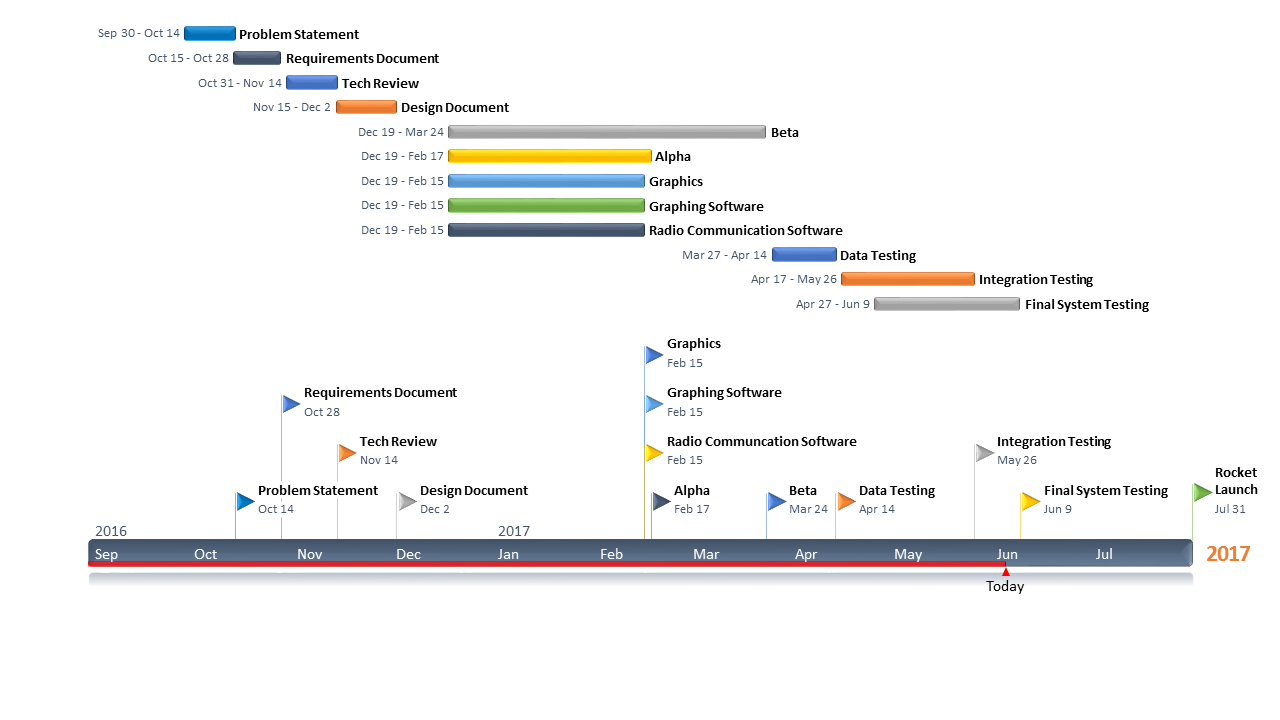
\includegraphics[scale=.50]{NewGanttChartHyro}
\end{figure}


\section{Original Design Document and Changes}
\begin{titlepage}
	\centering
	{\scshape\LARGE HyRo \par}
	%\vspace{1cm}
	{\scshape\LARGE Team 28\par}
	\vspace{1cm}
	{\scshape\Large Jason Klindtworth  |  Josh Asher  |   Layne Nolli}
	\noindent\makebox[\linewidth]{\rule{17cm}{2pt}}
	\vspace{1cm}
	{\huge\bfseries CS461\par}
	\vspace{2cm}
	{\Large\itshape Fall 2016\par}
	\vspace{4cm}
	{\large Software Design Document\par}\vspace{2cm}
	{\large Abstract\par}
	\vspace{1cm}
	High Altitude rockets have a distinct advantage in using Hybrid propulsion systems. These systems are complex and present challenges in remote telemetry including launch initialization and controlling remote fuel filling/disconnect. High altitude rockets contain an array of sensors that collect data which needs to be represented in human-readable format. The goal of HyRo is to provide solutionss for remotely launching and controlling the fuel systems on a hybrid propulsion system through onboard embedded circuitry/software that communicates with the launch team via radio waves. Our solutions will make use of embedded microprocessors on board the rocket, and a python-based GUI for ground teams to interface with. This circuitry/software will also transmit sensor data to the ground. Sensor data is displayed on our graphical user interface in an appealing, human-readable way. \par
	
	\noindent\makebox[\linewidth]{\rule{17cm}{2pt}}
	\vfill
	
	% Bottom of the page
	{\large \today\par}
\end{titlepage}


\setcounter{tocdepth}{2}

\section{Introduction}
\subsection{Scope}
This Design Document describes in detail, both the structure, and components of the HyRo deployment software system. It also includes the implementation details required to accurately and completely incorporate the specific requirements of this project as described in the Requirements Document. Because of the nature of the content in this document, it is assumed that the reader has familiarized themselves with the projects Requirements Document and is aware of the specific needs of this software package and graphical user interface. There is also an assumed general knowledge of computer programing. This document will rely heavily on the explanation of specific software functions and processes that will be designed in order to satisfy all of the requirements for this project. 
\subsection{Purpose}
This Design Document serves the following purposes:
\begin{itemize}
	\item To fully describe the structure, functions, data, and algorithms to be implemented in the software package.
	\item To identify specific and general system resources that will be utilized.
	\item To assist the HyRo team in the production and implementation of test cases.
	\item To verify full compliance with the requirements of the project.
	\item To aid the team in the general overview of the software package and what its capabilities are.
\end{itemize}
\subsection{Intended Audience}
The majority of the document is written for the benefit of software development and design professionals in order to gain specific knowledge of the HyRo software system and its capabilities. The intended audience for this documents is the HyRo team, including the following:
\begin{itemize}
	\item The project supervisor 
	\item The computer science sub-team working on the software package itself.
	\item The electrical engineering sub-team working on the hardware the software package will be incorporated into.
	\item the mechanical engineering sub-team working on the mechanical operations of the rocket which the software/hardware package will ride on.
	\item Any related sub-team for the project that requires knowledge of the computer system or interface system for the rocket.
\end{itemize}
\subsection{Definitions}
\begin{description}
	\item[Hybrid Rocket] A rocket with an engine that uses both solid and liquid fuel.
	\item[I/O] Input and Output.
	\item[PWM] Pulse Width Modulation is used to control signal level on a electrical wire.
	\item[Beagle Bone Black] A miniature computer that will be used on-board our hybrid rocket to house our software.
	\item[Python Dictionary] A associative array accessed by key value pairs.
	\item[Oxidizer] Liquid gas used to accelerate the burning of solid fuel.
	\item[Accelerometer] Measures acceleration.
	\item[Gyroscope] Measure tilt relative to the earth.
	\item[Magnetometer] Measures the electric field around it.
	\item[Multi Threaded] A program that runs multiple methods in parallel to the main program allowing components to run independently.
	\item[Mutex Lock] Used to lock control of an area of memory while an operation is completed. If any other parts of the system attempt to access this part of memory while the lock is in place they will not be allowed to.
	\item[Boolean] A way to represent a true or false value in software.
\end{description}
\subsection{Overview}
The HyRo software system is composed of two major components. The first component is housed on-board a hybrid rocket. This component is responsible for gathering sensor data from sensors on the the rocket, sending this data to a ground computer, and receiving commands from the ground system. These commands will interact with electrical components on the rocket. The second component of this system is software running on a traditional computer that is located on the ground near the launch site. This component is responsible for presenting the user with a graphical user interface that will allow the sending of commands to the rocket. It will also monitor data from the rocket that will be represented in graphs and gauges. The graphical user interface backend will also log any important information or commands that the rocket team requests. The main purpose of our project is to provide remote filling and data visualization. This paper is sectioned into 3 views. The first two views, System Architecture On-board the Rocket and System Architecture on the traditional computer, are explained from a logical viewpoint. The final section, the user interface, is explained from and interface viewpoint.
\section{Stake Holders and Concerns}
The primary stake holders in this project are Nancy Squires and the hybrid rocket team collectively. The rocket team is composed of Mechanical Engineering students, Electrical Engineering Students, and Computer Science Engineering students. We all have the same design concerns. These concerns include remotely filling and launching a rocket. The launching processes requires a sequence of command to complete. All commands and responses need to be logged in this process. Finally the most important thing is to be able to visualize sensor data while the rocket is in flight and again . This communication needs to be fast and accurate. This project is an ongoing process and its design will be a living entity. Things will change and we must adapt our design to these changes as the project progresses.
\section{System Architecture On-board the Rocket }	
The SDD module design of the software on-board the hybrid rocket detailed here after will explain the approach, methods, and properties of this component of the system. Software running on-board the rocket will communicate to software running on a traditional computer through a radio transceiver connected to the Beagle Bone Black. For convenience a diagram is provided below to show the entirety of the entire system. This section will  only cover the design of the software running on the Beagle Bone Black. \par

\begin{figure}[!ht]
	\caption{Data Flow Between System Components.}
	\centering
	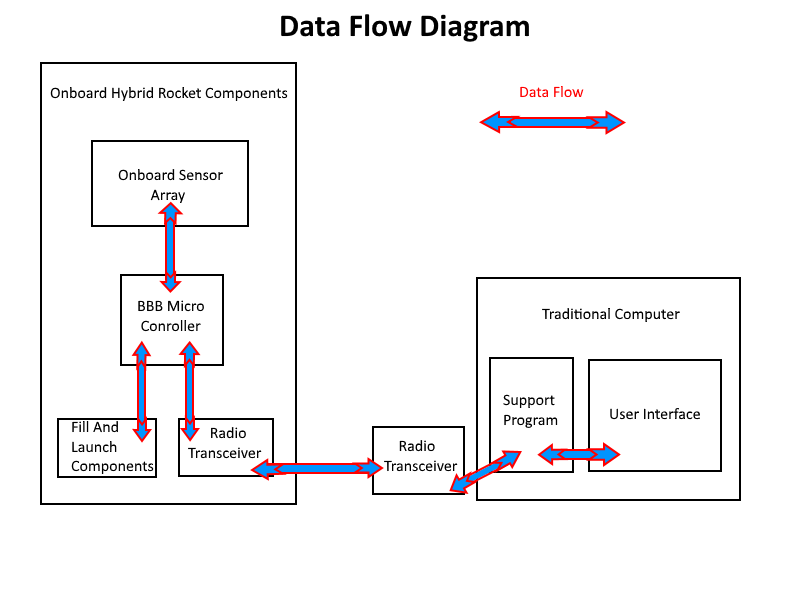
\includegraphics[scale=.85]{RocketBlockDiagram}
\end{figure}
\FloatBarrier

\subsection{Components} 
This section is intended to explain the electrical components of the rocket we will be receiving and/or sending data too. It is a general overview of what could be part of the system as the rocket has not yet been designed. Exact sensors are not presented because they yet to be chosen, though collection of data from them will be the same regardless. This allows for easy expansion of sensors in the code if time allows.\par
Based on current design plans the rocket will have an accelerometer, barometric/temperature sensor, and a servo to control filling, arming, and launching of the rocket. The sensors will be polled for data every 500 milliseconds and this data will be held in a buffer to be transmitted. Each sensor/servo has drivers built in python that will be used to access the sensors/servo data and in case of the servo sen PWM signals to control the movement of the servo.\par
The sensors and servo are connected to the Beagle Bone Black physically through I/O lines available on the board. The drivers define these connections and the functions to preform communication. There is a chance that the rocket design will change and we will need to create our own drivers for the new components. If that happens the driver design will be detailed under this section. At the moment all components used last year currently have drivers available.\par
\subsection{Data Format}
There are two buffers in this program. One to hold the sensor data and one to hold commands received. They are both globally available to the entire program.
\subsubsection{Sensor Data Buffer}
The sensor data buffer will be a python dictionary with keys relating to the name of the sensor output. For examples the temperature data will be stored in and accessed by the field "temperature".  The timestamps field is important to the radio transceiver polling function (detailed below) as this is what it uses to decide if the data is new. Some of these data items are not going to be used by the ground software, but are being recorded for future data visualization expansion.
\begin{description}
	\item[Buffer Name] dataBuffer
	\item[Buffer Keys]  -
	\begin{description}
		\item[time\_stamp] Time the current data was written to this buffer.
		\item[altitude] The altitude above ground level reading from the altitude sensor.
		\item[temp] The temperature reading from the temperature sensor.
		\item[a\_x] Accelerometer data from x axis.
		\item[a\_y] Accelerometer data from y axis.
		\item[a\_z] Accelerometer data from z axis.
		\item[g\_x] Gyroscope data from the x axis.
		\item[g\_y] Gyroscope data from the y axis.
		\item[g\_z] Gyroscope data from the z axis.
		\item[m\_x] Magnetometer data from the x axis.
		\item[m\_y] Magnetometer data from the x axis.
		\item[m\_z] Magnetometer data from the x axis.
		\item[tank\_pres] The pressure of the oxidizer tank.
		\item[chamber\_pres] The pressure of the combustion chamber
	\end{description}
\end{description}

\subsubsection{Command Buffer}
The command buffer will be used to store commands received from the ground computer software component to be accessed by the command thread. A python list data structure will be used to provide easy pushing and popping of values. When a command is detected it is added to this array and as it is processed it is removed from the array.\par
{\bf Buffer Name:} commandBuffer \\
{\bf Example:}\\
commandBuffer = {} // empty \\
New command Received = arm add to buffer \\
commandBuffer = {0 : 'arm'} \\
New command Received = disarm add to buffer \\
commandBuffer = {0 : 'arm', 1:  'disarm'} \\
Command Processed = 'arm' \\
commandBuffer = { 0 :'disarm'} \\
Command Processed = 'disarm' \\
commandBuffer = {} //empty \\


\subsection{Methods and Threads}
This component will be designed in using multi threaded approach with helper functions. Each thread will be responsible for a certain aspect of the system. They will communicate through the two buffers detailed above. This will require mutex locks be put on the buffers prior to any action taken from the independent threads. The following is a list of the threads and helper functions with their descriptions and interactions.
\subsubsection{Sensor Polling Thread}
{\bf Purpose:} \\
This thread is used to pull data from the sensors every 500 milliseconds. The data is then placed into the sensor data buffer. \par
{\bf Definition:} \\ 
sensor\_thread() \par
{\bf Inputs:} \\  Sensor data from the varies sensors. This is not a parameter input instead the function reads the data from the sensors as input.
{\bf Outputs:} \\ Sensor data to the sensor data buffer.
{\bf Process/Algorithm:} \\
When the thread starts it initially creates sensor objects to allow access to the sensors data through the use of their read functions. Afterwards this thread will run in a continuous loop. The loop will collect data from each of sensors in a temporary array until all sensors have been polled. Data is aquired by calling read or its equivalent of the related sensor object. When the thread has collected data from all sensors it will place a mutex lock on the sensor data buffer and write the new data to the buffer along with a time stamp. \par
\subsubsection{Command Processing Thread}
{\bf Purpose:} \\
The command processing thread will monitor for new commands in the commands buffer. If commands are received it will process them and take appropriate action. This could include sending an error message to the ground computer through the radio transceiver send function. \par
{\bf Definition:} \\ 
command\_thread() \par
{\bf Inputs:} \\  Data from the command buffer. \par
{\bf Outputs:} \\ Signals to servo and messages to rf\_send() \par
{\bf Calls:} \\ 
rf\_send(message)  \par
{\bf Process/Algorithm:} \\
When the thread initializes all servo objects will be instantiated to allow for access their corresponding electrical signal lines. The command processing thread will monitor the command buffer for new commands. If the command buffer length is not zero there is a new command in the buffer.The buffer will be checked  every 250 milliseconds for a new command. Commands will be processed through a set of conditional statements. Commands must be performed in a specific sequence detailed below next to the command explanation. Boolean flags will be used to determine if a command has been previously processed.  Each command will result in a call to the respective servo objects electrical signal line. This will cause the physical servo to change positions. The values output on the signal lines will be determined by the servo used. These details have not been solidified by the rocket team yet. Regardless the functionality will be the same only the values outputted will change once an appropriate device has been chosen. \par
If a command passes its conditional statement the servo function will be called on the appropriate servo object with a electrical signal value corresponding to its proper adjustments. The adjustment measurements will be determined by the mechanical engineers on the project and hard coded i]nto the software. After each command is successfully processed an acknowledgment will be sent to rf\_send(message) to inform the ground software a command was successfully processed. If a] command does not pass a conditional a message will be sent to radio transceiver by calling rf\_send(message) with the appropriate error message. The command will then be dropped and no action will be taken. Once the command sequence has been fulfilled the rocket is put into the launch state. This is dictated by a global boolean variable.\par
{\bf Commands:} \\
\begin{description}
	\item[fill] This will adjust a servo to fill the oxidizer tank before launch. Sequence number 1.
	\item[arm] This will adjust a servo prepare the rocket for ignition. Sequence number 2.
	\item[ignition] This will send a signal to igniter to ignite the rocket fuel. Sequence number 3.
	\item[launch] This will adjust a servo to release the rocket from its base. Sequence number 4.
	\item[disarm] This will adjust a servo to reverse the arming process. Can be used at any time.
	\item[abort] This will adjust all servos to their initial state. Can be used at any time.
\end{description}
\subsubsection{Radio Transceiver Thread}
{\bf Purpose:} \\
The radio transceiver thread is responsible for monitoring the radio transceiver for incoming data from the software running on the traditional computer. \par
{\bf Definition:} \\ 
comm\_thread() \par
{\bf Inputs:} \\  Data from the radio transceiver and data from the sensor data buffer. \par
{\bf Outputs:} \\ Data to the command buffer and data to be sent by the radio transceiver. \par
{\bf Calls:} \\ rf\_send(message) \par
{\bf Process/Algorithm:} \\
When the radio transceiver thread initializes it attempts to read from the radio transceiver every 100 milliseconds. At this point the rocket is in a the pre-launch state which is dictated by a boolean flag. While the rocket is in the pre-launch stage this thread will only poll the radio transceiver object for new messages. When a command is received it is placed into the command buffer by first putting a mutex lock on the buffer and pushing the new command onto the buffer. The thread will repeat this process until it detects that the pre-launch stage has passed.  \par
After the system has enter the launch stage this thread will change its behavior. Instead of monitoring for commands it will monitor the sensor data buffer for new data every 250 milliseconds. It detects new data by checking the time stamp value in the sensor data buffer dictionary. It initially stores the first time value and then upon finding a newer time value it will replace the old time value with the new time stamp and send the buffer into the radio transceiver by calling rf\_send(message) with the values from the dictionary as parameters. It repeats this process indefinitely. \par
\subsubsection{Main Thread}
{\bf Purpose:} \\
The main thread in the entry point into the software. It runs all initialization functions and starts all threads. \par
{\bf Definition:} \\ 
main() \par
{\bf Inputs:} \\  None \par
{\bf Outputs:} \\ None \par
{\bf Calls:} \\ init(), comm\_thread(), sensor\_thread(), command\_thread \par
{\bf Process/Algorithm:} \\
The main function calls the initialization function then creates the radio transceiver thread, the command processing thread, and the sensor thread. It will shut down all threads on program exit. \par
\subsubsection{Initialization Function}
{\bf Purpose:} \\
Initialize any servos, sensors, or global variables. \par
{\bf Definition:} \\ 
init() \par
{\bf Inputs:} \\  None \par
{\bf Outputs:} \\ None \par
{\bf Process/Algorithm:} \\
Initializes all global variables to default values. Then sets up any global comportments like servos to their default values defined by the mechanical engineering team. \par
\subsubsection{Radio Transceiver Send Function}
{\bf Purpose:} \\
Writes a message to send to the radio transceiver. \par
{\bf Definition:} \\ 
send\_rf(message) \par
{\bf Inputs:} \\  Message to send. \par
{\bf Outputs:} \\ Message to radio transceiver. \par
{\bf Process/Algorithm:} \\
Upon being called in turns calls the write function of the radio transceiver object with the message provided in the message parameter. 
\subsection{Rationale}
Our projects major functions are to get data from a rocket to a traditional computer and represent it visually. As far as the software running on the beagle bone black its main function is to process commands and transmit sensor data. The approach we have taken will allow for fast easy maneuvering of data by using a simply multi threaded process that will store the data directly in memory. The threads will allow for simultaneous operation of these features. The approach we chose is procedural instead of object oriented, but this is to provide simplicity. Our program will not be large compared to modern programs, but needs to perform specific tasks.
\subsection{Language}
We have chosen to use python because of its simplicity and strong API for USB reading and graphic rendering. It also is a stronger cross platform language then other options we explored. Another determining factor in this choice was last years success with this language.

\section{System Architecture on a Traditional Computer }
The SDD module design of the software running on a traditional computer detailed here after will explain the approach, methods, and properties of this component of the system. Software running on the traditional computer will communicate to the software detailed above running on-board the rocket. This component of the system will be responsible for monitoring radio transmissions, sending commands, logging, and the user interface back end. \par

\subsection{Overview}
In the following sections we describe the components of this software, excluding the user interface which is described in depth in the next section. We go over the graphical back end toolkits that will be used to draw the user interface, the data format of buffers and logs, worker threads, button listener functions, data conversion functions, and data visualization functions (drawing functions). \par

\subsection{GUI and Graphing Toolkits}
We will be using the Python TKinter library which provides a basis for windows, buttons, canvas, and other varies components we will need to create our graphical interface. This library includes event listeners to easily detect button presses and canvas to easily draw gauges and graphs. All sub components like buttons are called widgets in TKinter. \par
On top of Tkinter we will be using Matplotlib which is a graphical plotting library. Matplotlib provides functions to be easily able to graph data and scale those graphs. Graphs will be drawn on TKinter canvas widgets.\par

\subsection{Data Format}
\subsubsection{Sensor Data Buffer}
The sensor data buffer will be a python dictionary with keys relating to the name of the sensor output. For examples the temperature data will be stored in and accessed by the field "temperature".  The timestamps field is important to redraw function (detailed below) as this is what it uses to decided if the data is new.
\begin{description}
	\item[Buffer Name] dataBuffer
	\item[Buffer Keys]  -
	\begin{description}
		\item[time\_stamp] Time the current data was written to this buffer.
		\item[altitude] The altitude above ground level reading from the altitude sensor.
		\item[temp] The temperature reading from the temperature sensor.
		\item[accell] Accelerometer data from x axis.
		\item[velocity] Accelerometer data from y axis.
		\item[tank\_pres] The pressure of the oxidizer tank.
		\item[chamber\_pres] The pressure of the combustion chamber
	\end{description}
\end{description}
\subsubsection{Log Buffers}
Log buffers will hold previously received data for a particular key from the sensor data buffer. Each key (listed in the last section) will have its own buffer. As data is processed it will be placed into its log buffer. The log buffers will each hold up to 256 of the last entries. This is to allow time graphs to be plotted. These buffers are 2 dimensional arrays that hold that sensors value and a time stamp.
\begin{description}
	\item[Buffers]  -
	\begin{description}
		\item[altitude] The altitude above ground level reading from the altitude sensor.
		\item[temp] The temperature reading from the temperature sensor.
		\item[accell] Accelerometer data from x axis.
		\item[velocity] Accelerometer data from y axis.
		\item[tank\_pres] The pressure of the oxidizer tank.
		\item[chamber\_pres] The pressure of the combustion chamber
	\end{description}
\end{description}

\subsubsection{Command Response Message Format}
Command response message will be sent as a string with the command that is being responded too followed by a colon followed then by the response message from the on-board system. All commands have not been finalized by the rocket team, but will follow this format.  For example: \par
{\bf Launch: Sequence has not been followed. Rocket is not ready to launch. } \par

\subsubsection{Data Log Format}
When data is logged each entry will be place on a separate line in a text file. The line will consist of a time stamp and then a list of key value pairs from the data buffer. Key value you pairs will have an equal sign between them. The time stamps are formatted as follows: \par 
{\bf 6-1-2016:12:05:20} \par
Which represents Month-Day-Year : Hours : Minute : Second \par
Here is an example complete data log entry: \par
{\bf 6-1-2016:12:05:20 altitude="740" temp="70" accel="10" velcoity="15" tank\_pres="20" chamber\_pres="30"}\par

\subsubsection{Command Log Format}
When commands are logged each entry will be placed on a separate line of a text file. The line will consist of a time stamp followed by the command that was issued. Times stamps are in the same format as described in the previous section. Here is an example complete command log entry.\par
{\bf  6-1-2016:12:05:20 Abort}\par

\subsubsection{Response Log Format}
When responses are logged each entry will be placed on a separate line of a text file. The line will consist of a time stamp followed by the command that was responded to followed by a colon with the response to the command appended to the end. Times stamps are in the same format as described in the previous section. Here is an example complete response log entry.\par
{\bf  6-1-2016:12:05:20 Ignite:Sequence has not been followed. Rocket not ready to ignite.}\par

\subsection{Methods and Threads}
This component will be designed in using multi threaded approach with helper functions. Each thread will be responsible for a certain aspect of the system. They will communicate through the two buffers detailed above. This will require mutex locks be put on the buffers prior to any action taken from the independent threads. The following is a list of the threads and helper functions with their descriptions and interactions.
\subsubsection{Main Thread}
The main thread in the entry point into the software. It runs all initialization functions and starts all threads. \par
{\bf Definition:} \\ 
main() \par
{\bf Inputs:} \\  None \par
{\bf Outputs:} \\ None \par
{\bf Calls:} \\ init(), data\_thread, redraw\_thread \par
{\bf Process/Algorithm:} \\
The main function calls the initialization function then creates the data thread and the redraw thread. It will shut down all threads on program exit. \par
\subsubsection{Data Thread}
The data thread is responsible for polling the radio transceiver for new data or command responses messages. Then passing the data to converter functions or the command response message to the command response function.. \par
{\bf Definition:} \\ 
data\_thread() \par
{\bf Inputs:} \\  None \par
{\bf Outputs:} \\ New data to converter functions. \par
{\bf Calls:} \\ convTemp(data), convCHPressure(data), convAlititude(pressure, temp), convTankPressure(d), convAccell(data), convVelocity(data) \par
{\bf Process/Algorithm:} \\
The data thread continuously checks for data coming in on the radio transceiver by callings read on the radio transceiver object every 250 milliseconds. When a data packet arrives this thread processes the data by sending the value of the appropriator key to the appropriate data converter. For example the key "temperature" would be sent to the convTemp function. Which will handle the data from there on. If a command response message is received it is passed to the command response processing function.  \par
\subsubsection{Redraw Thread}
The redraw thread is responsible for monitoring for new converted data and passing the data to the appropriate redraw functions.\par
{\bf Definition:} \\
redraw\_thread() \par
{\bf Inputs:} \\  None \par
{\bf Outputs:} \\ None \par
{\bf Calls:} \\ drawTemp(data), drawCHPressure(data), drawAlititude(data), drawTankPressure(data), drawAccel(data), drawVelovity(data) \par
{\bf Process/Algorithm:} \\
The redraw function will check the time stamp value of the data buffer and if it is newer than the one it had previously recorded it will process the data. Upon detecting new data the redraw function will send each new data value to its appropriate draw function. The data at this point has already been converted for the drawing functions so it may be passed directly to them. For example it will pass the temperature data from the data buffer to the drawTemp() function. This thread is only responsible for data delivery to the temperature, chamber pressure, altitude, tank pressure, acceleration, and velocity redraw functions. Each draw function is responsible for graphing the data to its specific canvas.\par
\subsubsection{Radio Transceiver Send Function}
{\bf Purpose:} \\
Writes a message to send to the radio transceiver. \par
{\bf Definition:} \\ 
send\_rf(message) \par
{\bf Inputs:} \\  Message to send. \par
{\bf Outputs:} \\ Message to radio transceiver. \par
{\bf Process/Algorithm:} \\
Upon being called in turns calls the write function of the radio transceiver object with the message provided in the message parameter. \par
\subsubsection{Initialization Function}
{\bf Purpose:} \\
Initializes global buffers, global objects, global variables, and the user interface. \par
{\bf Definition:} \\ 
init() \par
{\bf Inputs:} \\ None. \par
{\bf Outputs:} \\None. \par
{\bf Process/Algorithm:} \\
This function initializes all global buffers, objects and variables to their default values. It then creates the window object, all button widgets, all canvas widgets for graphs, and the graphing menu widget and buttons. Once all user interface items have been initialized it calls the main windows drawing method to display the initial interface. This function is called before any of the threads in this component are started. \par

\subsubsection{Process Command Response Function}
{\bf Purpose:} \\
Receives command response messages from the data thread and processes them. This function will inform the user of any failed or out of sequence commands.  \par
{\bf Definition:} \\ 
command\_response(message) \par
{\bf Inputs:} \\  Command response to process. \par
{\bf Outputs:} \\ Logs responses to text file and message to screen. \par
{\bf Calls: drawMessage()}\par
{\bf Process/Algorithm:} \\
Upon receiving a command response message from the data thread this function opens the command response log and appends the message to the log with a newline. It then passes the message to the message draw function. \par

\subsubsection{Button Event Listeners}
Button listeners are provided by Tkinter as call back functions bound to the button the window. There will be two sets of button event listeners in the project. One set will be bound the the command buttons and the other to the graphing options buttons.
\paragraph{Command Button Listeners}
Each command button placed on the screen (shown in section 5) will have a function bound to it that will send the corresponding command string to the rf\_send() function. When a button is pressed that string is sent directly to the rf\_send function which in turns write it to the radio transceiver. If a command fails the rocket will send a error response. It is not the responsibility of these functions to make sure the command is in the correct order. Below is an example command button callback function. \\ \\
{\bf sendFill() }
\\  \\
Each button will have its own functions like this. In this example the sendFill() function will call the rf\_send() function with the message "filll".

\paragraph{Graphing Options Buttons}
Each graphing option button placed on the screen (shown in section 5) will have a function bound to it that will change the graph view of the multi functional graph window. When a graphing button is pressed it call its corresponding draw function that will replace the current graph in this window. Below is an example graphing option callback function: \\ \\
{\bf tempAsTimeClicked()} \\ \\
Each button will have its own functions like this. In this example the tempAsTimeClicked() function will call the drawTempAsGraph() function whitch will draw the temperature time graph in the multi functional graph window.

\subsubsection{Data Log Function}
{\bf Purpose:} \\
Logs the data it is passed to the data log text file.  \par
{\bf Definition:} \\ 
data\_log(data) \par
{\bf Inputs:} \\ Dictionary of data to log. \par
{\bf Outputs:} \\A line representing the data passed in to the data log text file. \par
{\bf Calls: drawMessage()}
{\bf Process/Algorithm:} \\
This function takes the data from data parameter and converts it to the data log format string. It then writes this string as a new line to the data log text file. \par

\subsubsection{Command Log Function}
{\bf Purpose:} \\
Logs the data it is passed to the command log text file.  \par
{\bf Definition:} \\ 
command\_log(data) \par
{\bf Inputs:} \\ Command to log. \par
{\bf Outputs:} \\A line representing the command passed in to the command log text file. \par
{\bf Calls: drawMessage()}
{\bf Process/Algorithm:} \\
This function takes the a command message from data parameter and converts it to the command log format string. It then writes this string as a new line to the command log text file. \par
\subsubsection{Converter Functions}
Each of the follow functions convert data they receive to the proper format for the drawing functions. They then store the data in the main data buffer for the drawing functions to access.  Each converter function is described in its specific details below. \par

\paragraph{Temperature Converter}
{\bf Purpose:} \\
Converts raw temperature sensor data to data suitable for the drawing functions.  \par
{\bf Definition:} \\ 
convTemp(data) \par
{\bf Inputs:} \\ Raw temperature data. \par
{\bf Outputs:} \\ Converted data to data buffer. \par
{\bf Process/Algorithm:} \\
This function receives data from the data thread in its data parameter to convert to a temperature value suitable for graphing. It then will store the converted temperature in the data buffer. It will convert the data by using a multiplier and offset provided on the data sheet of the temperature sensor.Temperature will be converted to Fahrenheit. \par

\paragraph{Chamber Pressure Converter}
{\bf Purpose:} \\
Converts raw pressure sensor data to data suitable for the drawing functions.  \par
{\bf Definition:} \\ 
convCHPressure(data) \par
{\bf Inputs:} \\ Raw chamber pressure data. \par
{\bf Outputs:} \\ Converted data to data buffer. \par
{\bf Process/Algorithm:} \\
This function receives data from the data thread in its data parameter to convert to a pressure value suitable for graphing. It then will store the converted pressure in the data buffer. It will convert the data by using a multiplier and offset provided on the data sheet of the pressure sensor used in the chamber of the rocket. Pressure will be converted to pounds per square inch. \par

\paragraph{Altitude Converter}
{\bf Purpose:} \\
Converts raw barometric pressure sensor readings to data suitable for the drawing functions.  \par
{\bf Definition:} \\ 
convAltitude(pressure, temp) \par
{\bf Inputs:} \\ Raw barometric pressure data. \par
{\bf Outputs:} \\ Converted data to data buffer. \par
{\bf Process/Algorithm:} \\
This function receives data from the data thread in two parameters. One is pressure and one is temperature, both required to calculate altitude. Altitude will be measured in feet.  It then will store the converted temperature in the data buffer. This conversion is currently provided as a function call in the current sensors library. If the design of the rocket changes the barometric pressure equation will have to be used. If that is the case that will be explained in this section. For now converting the temperature and pressure to altitude requires a call to the altitude conversion function which is part of the altitude sensor library. \par

\paragraph{Tank Pressure Converter}
{\bf Purpose:} \\
Converts raw pressure sensor data to data suitable for the drawing functions.  \par
{\bf Definition:} \\ 
convTankPressure(data) \par
{\bf Inputs:} \\ Raw tank pressure data. \par
{\bf Outputs:} \\ Converted data to data buffer. \par
{\bf Process/Algorithm:} \\
This function receives data from the data thread in its data parameter to convert to a pressure value suitable for graphing. It will convert the data by using a multiplier and offset provided on the data sheet of the pressure sensor used on the oxidizer tank of the rocket. Pressure will be converted to pounds per square inch. \par

\paragraph{Acceleration Converter}
{\bf Purpose:} \\
Converts raw accelerometer sensor data to data suitable for the drawing functions.  \par
{\bf Definition:} \\ 
convAccell(data) \par
{\bf Inputs:} \\ Raw acceleration data. \par
{\bf Outputs:} \\ Converted data to data buffer. \par
{\bf Process/Algorithm:} \\
This function receives data from the data thread in its data parameter to convert to an acceleration value suitable for graphing. The parameter will be a raw acceleration reading from the sensor. It will convert this to the Meters per second squared with the formula provided by the sensor manufacturer. This may include more math if the accelerometer API is not complete This will be added to this document if need be. It then will store the data in the data buffer. \par

\paragraph{Velocity Converter}
{\bf Purpose:} \\
Converts raw acceleration data to velocity data suitable for the drawing functions.  \par
{\bf Definition:} \\ 
convVelocity(data) \par
{\bf Inputs:} \\ Raw acceleration data. \par
{\bf Outputs:} \\ Converted data to data buffer. \par
{\bf Process/Algorithm:} \\
This function receives data from the data thread in its data parameter to convert to a velocity value suitable for graphing. The parameter will be a raw acceleration reading from the sensor. It will convert this to the Meters per second by first converting it to meters per second squared (normal acceleration) with the formula provided by the sensor manufacturer. Then it will take the integral of the acceleration to obtain the velocity.  It then will store the data in the data buffer. \par

\subsubsection{Drawing Functions}\
Each of the following drawing functions are called by the redraw thread when data becomes available to be displayed on the screen. They do not take data as input to be displayed, but instead read the data from the data buffer or the log buffer. Except for the message drawing routing it takes a input message to be drawn in the message window. Each function is responsible for a different data item and will display it according to the format of that data. The following is a list of the drawing functions and their specific operation.

\paragraph{Message Drawing Routine}
{\bf Purpose:} \\
Display command response message in the message window.  \par
{\bf Definition:} \\ 
drawMessage(message) \par
{\bf Inputs:} \\ Message string to draw.\par
{\bf Outputs:} \\Message to the message window. \par
{\bf Process/Algorithm:} \\
This function will take as its input parameter a command message and then draw the string in the message window of the user interface. \par

\paragraph{Temperature Drawing Routine}
{\bf Purpose:} \\
Draw the temperature data on the user interface.  \par
{\bf Definition:} \\ 
drawTemp() \par
{\bf Inputs:} \\None. \par
{\bf Outputs:} \\Temperature gauge on the user interface.\par
{\bf Process/Algorithm:} \\
This function will pull temperature data from the data buffer and draw a gauge representing the data on the temperature canvas. \par

\paragraph{Chamber Pressure Drawing Routing}
{\bf Purpose:} \\
Draw chamber pressure on the user interface. \par
{\bf Definition:} \\ 
drawCHPressure() \par
{\bf Inputs:} \\None. \par
{\bf Outputs:} \\Chamber pressure gauge on the user interface.\par
{\bf Process/Algorithm:} \\
This function will pull chamber pressure data from the data buffer and draw a gauge representing the data on the chamber pressure canvas. \par

\paragraph{Altitude Drawing Routine}
{\bf Purpose:} \\
Draw rocket altitude on the user interface. \par
{\bf Definition:} \\ 
drawAltitude() \par
{\bf Inputs:} \\None. \par
{\bf Outputs:} \\Altitude gauge on the user interface.\par
{\bf Process/Algorithm:} \\
This function will pull altitude data from the data buffer and draw a gauge representing the data on the altitude canvas. \par

\paragraph{Tank Pressure Drawing Routine}
{\bf Purpose:} \\
Draw oxidizer tank pressure on the user interface. \par
{\bf Definition:} \\ 
drawTankPressure() \par
{\bf Inputs:} \\None. \par
{\bf Outputs:} \\Oxidizer tank pressure gauge on the user interface.\par
{\bf Process/Algorithm:} \\
This function will pull tank pressure data from the data buffer and draw a gauge representing the data on the tank pressure canvas. \par

\paragraph{Acceleration Drawing Routine}
{\bf Purpose:} \\
Draw acceleration graph on the user interface. \par
{\bf Definition:} \\ 
drawAccell() \par
{\bf Inputs:} \\None. \par
{\bf Outputs:} \\Acceleration graph on the user interface.\par
{\bf Process/Algorithm:} \\
This function will pull acceleration data from the data buffer and draw a graph representing the data on the acceleration canvas. \par

\paragraph{Velocity Drawing Routine}
{\bf Purpose:} \\
Draw velocity graph on the user interface. \par
{\bf Definition:} \\ 
drawVelocity() \par
{\bf Inputs:} \\None. \par
{\bf Outputs:} \\Velocity graph on the user interface.\par
{\bf Process/Algorithm:} \\
This function will pull velocity data from the data buffer and draw a graph representing the data on the velocity canvas. \par

\paragraph{Draw Temperature as Graph Routine}
{\bf Purpose:} \\
Draws temperature vs time as graph on the user interface. \par
{\bf Definition:} \\ 
drawTempAsGraph() \par
{\bf Inputs:} \\None. \par
{\bf Outputs:} \\Temperature vs time graph on the user interface.\par
{\bf Process/Algorithm:} \\
This function will take multiple data points from the temperature log buffer and plot them with their timestamps on the user interface in the time graph canvas.  \par

\paragraph{Draw Chamber Pressure as Graph Routine}
{\bf Purpose:} \\
Draws chamber pressure vs time as graph on the user interface. \par
{\bf Definition:} \\ 
drawCHPAsGraph() \par
{\bf Inputs:} \\None. \par
{\bf Outputs:} \\Chamber pressure vs time graph on the user interface.\par
{\bf Process/Algorithm:} \\
This function will take multiple data points from the chamber pressure log buffer and plot them with their timestamps on the user interface in the time graph canvas.  \par

\paragraph{Draw Altitude as Graph Routine}
{\bf Purpose:} \\
Draws altitude vs time as graph on the user interface. \par
{\bf Definition:} \\ 
drawAltAsGraph() \par
{\bf Inputs:} \\None. \par
{\bf Outputs:} \\Altitude vs time graph on the user interface.\par
{\bf Process/Algorithm:} \\
This function will take multiple data points from the altitude log buffer and plot them with their timestamps on the user interface in the time graph canvas.  \par

\paragraph{Draw Tank Pressure as Graph Routine}
{\bf Purpose:} \\
Draws tank pressure vs time as graph on the user interface. \par
{\bf Definition:} \\ 
drawTankPAsGraph()\par
{\bf Inputs:} \\None. \par
{\bf Outputs:} \\Tank pressure vs time graph on the user interface.\par
{\bf Process/Algorithm:} \\
This function will take multiple data points from the tank pressure log buffer and plot them with their timestamps on the user interface in the time graph canvas.  \par

\subsection{Rationale}
This part of our system reads and sends data. A big part of this decision was the choice on Python. There are great graphics libraries available for Python that are tailored to our needs. This will provide us with and easy to use and build graphical user interface. The back in is a procedural based multi threaded system that provides simplicity and easy data access.
\subsection{Language}
We have chosen to use python because of its simplicity and strong API for USB reading and graphic rendering. It also is a stronger cross platform language then other options we explored. Another determining factor in this choice was last years success with this language.

\section{User Interface Design}
The graphical user interface is the driving force behind this entire project. It may not seem as complicated as some modern interfaces, but its serves a very important purpose. The purpose is to visually represent data from a hybrid rocket and provide button to issue the rocket commands. These functions have been lacking in previous years rockets team and are the reason we were brought on board this project. Detailed in the following sections are these sections of the user interface. \par

\begin{itemize}
	\item The Command Buttons
	\item The Message Frame
	\item The Graphing Options Buttons
	\item The Gauges and  Graphs
\end{itemize}

\subsection{Drawing of Complete Screen}
Here is a basic drawing of the entire screen. This drawing will be replaced with a screen shot once the program has reached a stage where the components are all visible.\par

\begin{figure}[!ht]
	\caption{Mock up of the graphical user interface}
	\centering
	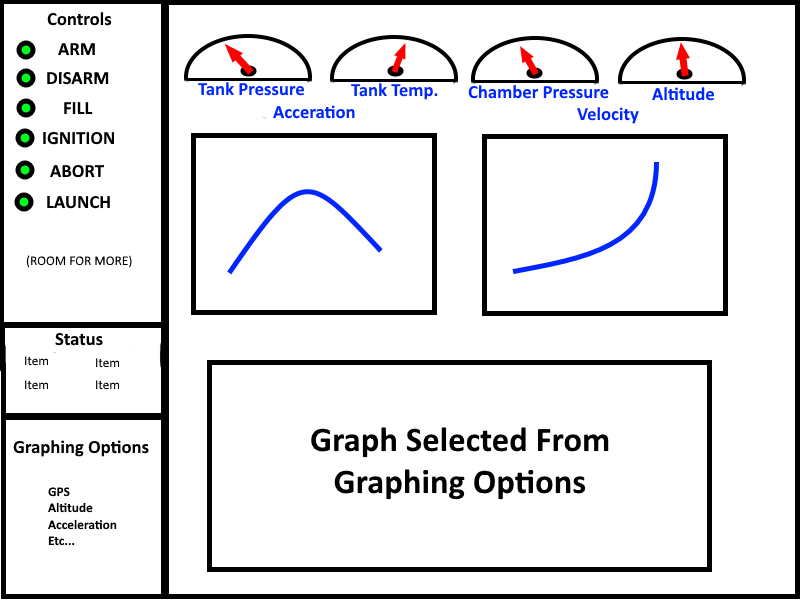
\includegraphics[scale=.85]{HyRoUIMockup}
\end{figure}

\subsection{The Command Buttons}
The command buttons are housed on the left side of the screen as depicted in the image above. These buttons will cause a command to be sent through the radio transceiver on the traditional computer to the radio transceiver on-board the rocket. The rocket will process the command and send a response back to be displayed in the message frame. The command buttons and their descriptions are as follows.\par

\begin{description}
	\item[Fill] This will attempt to initiate the oxidizer fill process while the rocket is on the ground.
	\item[Arm] This will adjust a servo prepare the rocket for ignition. Sequence number 2.
	\item[Ignition] This will send a signal to igniter to ignite the rocket fuel. Sequence number 3.
	\item[Launch] This will adjust a servo to release the rocket from its base. Sequence number 4.
	\item[Disarm] This will adjust a servo to reverse the arming process. Can be used at any time.
	\item[Abort] This will adjust all servos to their initial state. Can be used at any time.
\end{description}

\subsection{The Message Frame}
This is a small message box on the left hand side of the user interface directly under the command buttons. This box will display response message from the rocket. As message come in they will be appended to this message box. The box will be able to scroll if the messages exceeded the size of the frame.\par

\subsection{The Graphing Options Buttons}
These buttons are located on the left side of the user interface under the message frame. Each button will correspond to a specific graphing capability. When clicked on there will change which graph is displayed in the multi functional graphing window. Buttons and their corresponding graphs are listed below. \par

\begin{description}
	\item[Chamber Pressure vs. Time] Clicking this button will change the multi function graph window to a graph of chamber pressure vs. time
	\item[Altitude vs. Time] Clicking this button will change the multi function graph window to a graph of altitude vs. time.
	\item[Tank Pressure vs. Time] Clicking this button will change the multi function graph window to a graph of tank pressure vs. time.
	\item[Temperature vs. Time] Clicking this button will change the multi function graph window to a graph of temperature vs. time.
	
\end{description}

\subsection{The Gauges and Graphs}
Taking up most of the user interface on the right hand side are the gauges and graph canvases. Currently their will be 4 gauges that look like traditional gauges you would see on car dash board. They will be a semi circle with marks representing possible values of the data item. A arrow will be draw to represent the current value of the data. Below those gauges are two graphs representing velocity and acceleration these will graph these two data items vs time. Below the velocity and acceleration graphs is the multi function graphing window. This will display a user selected graph from the graphing options buttons selection menu. This will default to altitude vs time. Listed below are the gauges, graphs, and their units.

\subsubsection{Tank Pressure Gauge}
{\bf Units} \\ Tick marks are measured in pounds per square inch from 0 to 2000.\par
{\bf Description} \\ This gauge represents the current pressure of the oxidizer tank. It will rise and fall along with the tank pressure. This value can also be graphed in the multifunction window.\par

\subsubsection{Temperature Gauge}
{\bf Units} \\ Tick marks are measured in degrees Fahrenheit from 32 to 7000.\par
{\bf Description} \\ This gauge represents the temperature wherever the temperature sensor is located. It will rise and fall along with the temperature surrounding the temperature sensor. This value can also be graphed in the multifunction window. \par

\subsubsection{Chamber Pressure Gauge}
{\bf Units} \\ Tick marks are measured in pounds per square inch from 0 to 2000.\par
{\bf Description} \\ This gauge represents the pressure of the combustion chamber of the rocket. It will rise and fall along with the chamber pressure of the rocket. This value can also be graphed in the multifunction window. \par

\subsubsection{Altitude Gauge}
{\bf Units} \\ Tick marks are measured in feet above sea level from 0 to 15000.\par
{\bf Description} \\ This gauge represents the altitude of the rocket. It will rise and fall along with the altitude of the rocket. This value can also be graphed in the multifunction window. \par

\subsubsection{Acceleration Graph}
{\bf Units} \\ The x axis of the graph will be measured in meters per second squared and the y axis will be time from launch in seconds.\par
{\bf Description} \\ This graph represents the acceleration of the rocket with respect to time. The graph will be able to slide if the amount of data points exceeds the size of the graph window. \par

\subsubsection{Velocity Graph}
{\bf Units} \\ The x axis of the graph will be measured in meters per second and the y axis will be time from launch in seconds.\par
{\bf Description} \\ This graph represents the velocity of the rocket with respect to time. The graph will be able to slide if the amount of data points exceeds the size of the graph window. \par

\subsubsection{Multi Function Graph}
{\bf Units} \\ The x axis of the graph will be measured in different units depending on the graph chosen and the y axis will be time from launch in seconds.\par
{\bf Description} \\ This multi function graph will be the place where user selected graphing items are displayed. \par

\section{Summary}
The previous section have in detailed described our hybrid rockets software system. We have described how we will collect sensors data, send sensor data, receive and act on commands, and provide  a command and visualization interface for the rocket team members on the ground. We have detailed the data formats, log formats, radio transceiver routines, data conversion routines, drawing routines and the threads that will control all these components. These are all housed in a threaded procedural system for simplicity and speed. All these components combined will allow for remote filling, launching, and data visualization of a hybrid rocket. \par

\newpage

\section{Bibliography}
\begin{thebibliography}{9}
	
	\bibitem{BBB}
	BeagleBone.org,\\
	\emph{(Tues November 29 2016)},\\
	\emph{Beagle Bone Black product information and website},\\
	URL  http://beagleboard.org/black \\
	
	\bibitem{ExampleSDD}
	Unimap.edu example SDD,\\
	\emph{(Tues November 29 2016)}, \\
	\emph{Unimap software development examples}, \\
	URL http://portal.unimap.edu.my/portal/page/portal30/Lecturer\%20Notes/KEJURUTERAAN\_KOMPUTER/Semester\%202\%20Sidang\%20Akademik\%2020112012/EKT420\%20Software\%20Engineering/Example\%20of\%20Software\%20Design\%20Document(SDD)/EDDISS.pdf \\
	
	\bibitem{IEE1016}
	IEE 1016 Software Design Specifications,\\
	\emph{(Tues November 29 2016)}, \\
	\emph{IEE 1016 Document availble on campus}, \\
	
	\bibitem{TKinter}
	Python.org wiki,\\
	\emph{(Tues November 29 2016)}, \\
	\emph{Tkinter python wiki on python.org}, \\
	URL https://wiki.python.org/moin/TkInter\\
	
	\bibitem{Matplotlib}
	Matplotlib.org,\\
	\emph{(Tues November 29 2016)}, \\
	\emph{Matplotlib.org website documentation}, \\
	URL http://matplotlib.org/
	
\end{thebibliography}

\subsection{Changes in the Design}
There were many changes in the design over the course of the year. From big to little. The main thing that changed was that we did not have to do the onboard software of the avionics bay. This cut out all the material we had planned for, for that component. This as sad but gave us more time to focus on the other half which was a blessing. This left us with only the system component on the traditional computer. The whole first section of this document wasn't needed. For future reference it might be a good jumping point for anyone that does implement that part of this system in their project. \par
We ended up focusing on the user interface and its back end system. We did end up using tkinter and matplotlib they worked excellently. We had planned this elaborate system of buffers and log buffers, but ended up using python queues. We should of looked this up during the tech review, but in the process of coding stumbled across them. They ended up being thread safe and very easy to use. There ended up being a queue for each sensor data item that served as the data buffer and the log buffer. \par 
The data format ended up being changed by the ECEs and we followed suit with what they had which was "timestamp;temperature;pressure;altitude;acceleration\_x;acceleration\_y;acceleration\_z;gps\_latitude;gps\_longitude". The data log format ended up being a lot different. That whole idea changed; originally we were going to log the data in the format above in a single file. In the process of development we came up with a better idea. We decided to put each run in a time stamped folder where each data item would have its own log file. The format of the file would be time,data separated by newlines. This made it very easy for the drawing functions to reload data and to load an entire graph of data. It also cut down on the system memory we were using. \par
The main thread ended up being the logging and redrawing thread combined into one. After all the initialization we wait for the user to use a start button to begin radio transmission, drawing, and logging. The the start and stop buttons came along after we had got our program to beta. We realized that starting the program and begging everything instantly was the not he best way to go. The start/stop buttons allow the user to record multiple runs in one start of the program. In the main thread we begin a continuous loop that is stopped when the user clicks stop. In this loop we monitor for data items in the queues. When data comes in it is removed from the queue, drawn to the screen, and recorded in its individual log. We also provide a load button that allows the user to select a timestamped folder from a previous run. This will immediately display all the data from that run on the graphs.\par
The only difference in the drawing functions from our original design was that they read from a file, that also serves as the log file. This proved to be very effective and allowed us not to store to much information in core memory. The UI itself ended up changing a  bit. We had to remove all the buttons except for the fill button. We no longer needed the message frame and instead of graphing options we put all the data on the screen with graphs. Originally we were going to allow you to switch them, but there was enough room for everything. We had to remove one gauge (tank pressure) since the team did not put a sensor in for that. \par
There were a lot of changes to the design, most of witch occurred during development. We were all learning python as we went and as we were coding found better ways to handle things. The requirements also changed which effected what we needed to have on our UI. Overall I would have to say the fundamental ideas behind everything stayed the same. It was the details of putting them together that really changed. We ended up with a fairly small and elegant code base which you can find in appendix one. \par

\begin{titlepage}
	\centering
	{\scshape\LARGE HyRo \par}
	%\vspace{1cm}
	{\scshape\LARGE Team 28\par}
	\vspace{1cm}
	{\scshape\Large Jason Klindtworth  |  Josh Asher  |   Layne Nolli}
	\noindent\makebox[\linewidth]{\rule{17cm}{2pt}}
	\vspace{1cm}
	{\huge\bfseries CS461\par}
	\vspace{2cm}
	{\Large\itshape Fall 2016\par}
	\vspace{4cm}
	{\large Technology Review\par}
	\vspace{4cm}
	{\large Abstract\par}
	\vspace{1cm}
	It is important when begging to design a system to brainstorm options for each sub component. Certain technologies immediately pop into your mind when thinking of a solution to a problem, but it is important to make sure what you thought of was the best solution. This document is a way to compare possible technologies for the individual components of our solution and research which one would be the better choice. We do not want to reinvent the wheel when there is already a solution. We might also find a better solution when we conduct our research. This paper will lead us into our design with a better idea as to how we will accomplish HyRo.\\
	\noindent\makebox[\linewidth]{\rule{17cm}{2pt}}
	
	\vfill
	
	% Bottom of the page
	{\large \today\par}
\end{titlepage}
\tableofcontents

\section{Introduction}
We are desiginging a data driven user interface. Data will be collected from a hyrbrid rocket's sensors and passed through radio waves for us to visually represent on a screen. The users will be able to interact with the data and send data into the system in the form of rocket commands. To get a grasp on what technologies or methodologies we present to you our technology reviews. As a team we split the project into 10 sections that we will be responsible for. Each of these sections was carefully thought over and reviewed with 3 possibly technologies that could be used to build that section. The section and the people responsible are as follows: Generating and Capturing of Data on a Micro Controller (Joshua Asher), Generating and Capturing of Data on a Traditional Computer (Joshua Asher), Handling and Storage of Data (Joshua Asher), Processing Data to make it Suitable for Visualization and Storage(Joshua Asher), the toolkit to generate the UI (Jason Klindtworth), Visualization Tool Kit to Display Data in UI (Jason Klindtworth), The organization of the UI (Jason Klindtworth), Interaction Modes(Layne Nolli), UI Interaction Model(Layne Nolli), Mapping of Data onto Display Model (Layne Nolli). 

\section{Technology Reviews}
\subsection{Generating and Capturing of Data on a Micro Controller}
Onboard the hybrid rocket there will be a collection of sensors, controllers, and a radio transceiver that data will need to be collected from and transferred too. A micro controller will be connected to all these devices to collect and transfer this data amongst components. There are multiple options to choose from when it comes to which micro controller to choose and what API to access the communication port with. Different languages allow for access to different APIs to communicate with system devices.The three options being examined in this section are as follows. \\
\subsubsection{Options}

\begin{itemize}
	\item Using the Python Language and its API (PyUSB) to serial communications ports and GPIO lines with the Beagle Bone Black (BBB) micro controller.
	\item Using the C/C++ Language and its API to serial communications ports and GPIO lines with the Beagle Bone Black micro controller.
	\item Using either C/C++ or Python on a different micro controller like the RaspberryPI 3.\\
\end{itemize}

\subsubsection{Goals}
The goals in choosing the technology to generate and capture data on a micro controller are (1) choose a technology with simplicity as to allow data to be easily captured and generated. (2) To choose a technology that can communicate do these functions quickly (3) To choose a reliable platform that is not prone to errors. \\
\subsubsection{Criteria}
The criteria that these choices will be based on are: speed of language, complexity of communications USB API, complexity or existence of GPIO API, Processor of Micro Controller, amount of RAM on micro controller, amount of long term memory on micro controller, and other capabilities or packages the micro controller comes with.\\
\subsubsection{Comparison Table} 
The next two tables compare criteria between the 3 options.[1][2][4]\\ \\
\begin{table}
\centering
\begin{tabular}{ |p{2cm}|p{2cm}|p{2cm}| p{2cm}|p{2cm}| }
	\hline
	\multicolumn{5}{|c|}{Criteria Comparison Table 1} \\
	\hline
	&Speed of Language&Complexity of USB API&Processor&RAM\\
	\hline
	Python on BBB&Medium &Medium&AM335x 1GHz ARM Cortex-A8&512MB DDR3L (800 MHZ) \\
	\hline
	C/C++ on BBB &Fast& Medium&AM335x 1GHz ARM Cortex-A8&512MB DDR3L (800 MHZ)t \\
	\hline
	Raspberry PI 3 with either language &Medium or Fast&Medium&1.2GHz 64-bit quad-core ARMv8&1GB LPDDR2 (900 MHz) \\
	\hline
\end{tabular}
\end{table}
\\ \\ This next table is an extension to the previous. \\ \\
\begin{table}
	\centering
\begin{tabular}{ |p{2cm}|p{2cm}|p{2cm}| p{2cm}| }
	\hline
	\multicolumn{4}{|c|}{Criteria Comparison Table 2} \\
	\hline
	&Long Term Memory&Other capabilities/packages&Price of Micro Controller\\
	\hline
	Python on BBB &4G Embedded + MicroSD expansion&69 GPIO, I2C, 4 Serial Ports (lots more not specific to the project)&\$55 \\
	\hline
	C/C++ on BBB &4G Embedded + MicroSD expansion&69 GPIO, I2C, 4 Serial Ports (lots more not specific to the project)&\$55 \\
	\hline
	Raspberry PI 3 with either language &MicroSD Storage &17 GPIO &\$40 \\
	\hline
\end{tabular}
\end{table}
\vspace{1cm}
\subsubsection{Discussion}
Using the Python Language and its API (PyUSB) to serial communications ports and GPIO lines with the Beagle Bone Black (BBB) micro controller will provide a reasonably fast system with plenty of storage at a slightly higher price. One of the main allures to this option is Python. Python tends to allow for faster development time because of its simplistic syntax and well documented USB interface, PyUSB [PyUSB]. Python tends to run slower than C or C++ which can be used on this platform to accomplish the same goals, but results from last year show that it works at an adequate speed to perform serial communication and GPIO communication. Another pusher for Python is that last year’s team used it as the language for their system. PyUSB shares a similar complexity to libusb which C or C++ would use. Either choice would have an appropriate learning curve. Using Python would make the code very readable to future teams, but does suffer some in performance. The micro controller environments that Python runs on will have an accept on performance also. Python Running on the BBB has the advantage of access to more communication ports than it would on the Raspberry PI 3. The processing power is slightly less than that of the PI, but we do benefit from fast on board flash storage where our software can run. [3]\par
Using the C/C++ Language and its API to serial communications ports and GPIO lines with the Beagle Bone Black micro controller would provide faster serial and GPIO communication than using Python. Running on the BBB C/C++ would have access to the same environment as Python and the only other major benefit beside speed would be memory control. C/C++ provides the ability to access and store memory in more detail/control than Python does. Since we are not planning on any operations that are memory or CPU intensive I did not include this as criteria. C/C++ would be more time consuming and complex than Python, but not to a large degree. This would also have to be built from scratch, but in the end, would provide faster communication. This might not be required if the speed of the controllers, sensors, or radio transceiver are not as fast as the C/C++ software could produce. This will be tested down the road when the system begins to be built. [3][5]\par
Using either C/C++ or Python on a different micro controller like the RaspberryPI 3 is listed as an option to compare the abilities of a different micro controller to the one that was used last year. First of the RaspberryPI 3 is at least \$15 cheaper than the BBB. It also has a processor that is more powerful (that is judging the speed and core count) than the BBB. The quad core would be great for multithreading and there is twice as much RAM on the RaspberryPI. Though, it uses DDR2 which has half	the number of transfer per cycle than DDR3. I believe the RaspberryPI would be a great cheaper solution, but it does not support as many low-level communications ports as the BBB. The BBB has also been proven a successful option from last years’ experience.\\

\subsubsection{Beagle Bone Black with Python and PyUSB}
It was not easy to decide on which combination of these technologies would be the best for our Hybrid rocket system. The major influencing factor on my decision is that the team already has access to a BBB from last year and that component would not have to be purchased again this year. Further the team last year started to develop on this board using the Python language as the solution to collecting and generating data last year successfully. This has influenced me to choose this combination for this year's Hybrid rocket onboard system. C/C++ might be faster but this is not significant enough to merit a switch to those languages.\par

\subsection{Generating and Capturing of Data on a Traditional Computer}
On the other end of our system we will need to communicate with a USB device on a traditional computer to collect and pass generated data. There are many different APIs to access the serial devices connected to a computer depending on language and operating system. We could be targeting Windows or Linux when we build this software. 
The three options being examined in this section are as follows. \\
\subsubsection{Options}
\begin{itemize}
	\item Using Python with PyUSB on either Windows or Linux.
	\item Using C++/C\# with WinUSB on Windows.
	\item Using C/C++ with libusb on Linux..\\
\end{itemize}
\subsubsection{Goals}
The goals in choosing the technology to generate and capture data on a traditional computer are (1) choose a technology with simplicity as to allow data to be easily captured and generated. (2) To choose a technology that can communicate do these functions quickly (3) To choose a technology that can run under a single operating system at minimum, but be preferable to run under at least 2 different operating systems. \\
\subsubsection{Criteria}
The criteria that these choices will be based on are: speed of language, complexity of communications USB API, and the ability for the technology to run on at multiple operating systems.\\
\subsubsection{Comparison Table}
Comparison of Options vs criteria \\ \\
\begin{table}
\centering
\begin{tabular}{ |p{2cm}|p{2cm}|p{2cm}| p{2cm}| }
	\hline
	\multicolumn{4}{|c|}{Criteria Comparison Table} \\
	\hline
	&Speed of Language&Complexity of USB API&Ability to run on multiple operating systems\\
	\hline
	Using Python on Windows or Linux&Medium&Medium&Yes, with only slight modifications. \\
	\hline
	Using C/C++ on Windows&Fast&Medium&Only Windows \\
	\hline
	Using C/C++ Windows or Linux &Fast&Medium&Yes, depending on the presence of OS specific code in the software. \\
	\hline
\end{tabular}
\end{table}
\vspace{1cm}
\subsubsection{Discussion}
Using Python with PyUSB on either Windows or Linux provides a slower, but easy to access serial interface that will meet requirements in this part of the project. Python does not preform as fast as C/C++ when compared in bench marks, but its performance will be adequate for our situation. It also provides quicker development times and code that is easier to read. Python would coincide with the language chosen to be used on the BBB and if the Python is chosen for visualization. It’s preferable to have all the pieces of the software written in the same language. Python also provides a API that can be easily ported between Windows and Linux allowing us to potentially run our software on multiple operating systems with only slight modifications.[7] \par
Using C++/C\# with WinUSB on Windows would promise to be faster than running python on Windows. WinUSB is well documented and has many examples to help someone get started with USB communication. This would be a good option if the only desired operating system is Windows.  If performance becomes a problem this would be a good option also. It is however preferable to have a cross compatible solution as the engineering team tends to use both Windows and Linux, so this option does not stand a high chance of being chosen. \par
Using C/C++ with libusb on Windows or Linux provides both a speed boost and cross platform capabilities.  Libusb is well document with examples to get started and is provenly reliable interface. This option would be the fastest amongst the three if speed starts becoming an issue. It also may be over kill, there are no serious processor operations we must perform which C/C++ executes must faster. It is also more complex than writing code in Python, but doable if desired. This option has a lot of history in similar data collecting and gathering applications .[5][6] \\

\subsubsection{Python with PyUSB}
I have selected to use Python with PyUSB that provides a reasonable fast USB access coupled with the ability to be easily portable between Windows and Linux. Using libusb with C/C++ would be the faster and cross compatible, but most of the other code in this project has chosen Python and we want to keep everything in the same language if possible. Designing the product just for windows using WinUSB is too restrictive and option 2 is not going to be considered. Last yea'’s Python code was successful and already has code available that can be improved on. No sense in re-inventing the wheel.
\subsection{Handling and Storage of Data}
We must handle and store data from user input, sensors/controls input/output, and radio transceiver input/output.  We must record user commands and sensor data to the hard drive of the traditional computer. This part describes 3 methodologies of how to accomplish these tasks.The three options being examined in this section are as follows. \\
\subsubsection{Options}
\begin{itemize}
	\item Option 1: Buffer data in memory, process the data, then record the data that has been made suitable for reading to a text file for later retrieval.
	\item Option 2: Buffer data in memory, process the data, then send the data to a SQL database for storage and later retrieval.
	\item Option 3: Do not buffer data but instead directly write data to hard drive on computer and have that data accessible through a file descriptor.\\
\end{itemize}
\subsubsection{Goals}
The goals in choosing the technology to handle and store data are (1) to deliver data to the visualization/storage algorithms quickly (2) to allow the visualization/storage algorithms to easily access data (3) to save the data in long term storage (4) make the data in long term storage easy to access and understand.\\

\subsubsection{Criteria}
The criteria that these choices will be based on are: speed, ease of access for visualization, ease of access for long term data, and complexity introduced into software.\\
\subsubsection{Comparison Table}
Comparison of Options vs criteria (Options are labeled with corresponding tag from section a). \\ \\
\begin{table}
	\centering
\begin{tabular}{ |p{2cm}|p{2cm}|p{2cm}| p{2cm}|p{2cm}|  }
	\hline
	\multicolumn{5}{|c|}{Criteria Comparison Table} \\
	\hline
	&Speed&Ease of Access for Visualization/Storage&Ease of Access for Long Term Data&Complexity introduced into software\\
	\hline
	Option 1&Fast&Easy/Fast&User needs to read text files one by one.&Trivial and uses simple techniques like file descriptors to pass data. \\
	\hline
	Option 2&Medium&Easy/Fast&User would need to make queries to database, but data might be easier to select and retrieve.&Less Trivial as data in memory would have to be accessed and written to a SQL database. Providing more overhead and complexity to the program.\\
	\hline
	Option 3&Slow&Harder/Slower&Data would be hard to read and need further processing down the road.&This would add the most complexity and code would be more convoluted. \\
	\hline
\end{tabular}
\end{table}
\vspace{1cm}
\subsubsection{Discussion}
Buffering data in memory, processing the data, then recording the data that has been made suitable for reading to a text file for later retrieval is a great option. It would be the fastest code with less overhead than the other options for these reasons. One, it would not have to communicate with an outside data base and incur the overhead brought on by an extra API.  Two, it is fast to write data to text files and easy to replay the data into the visualization program. If the data is kept in a format that would could be easily read by our visualization system, it could be viewed repeatedly. The text file would be harder for humans to read than queries from and SQL database, but then you would have to have someone with knowledge of the SQL database to format the data. The complexity of this option is the simplest of the three options. We would put data in memory to be accessed by both the logging and visualization systems. Once both have used the data its memory can be recycled. Operations retrieving this data are very fast from memory. Transferring the data to a file would require simple file descriptor read/write access and an appropriate formatting definition to make the logged information readable.\par
Buffering data in memory, processing the data, then sending the data to a SQL database for storage and later retrieval is another viable option. The plus side of this option would be the ease of representing different forms or data using database tables and entries. These later can be taken and queried from in specific ways to present data that is requested. This would allow better data visualization in the long run, but would require a database access software to be written. This is now out of the scope of our project. It would be a good goal for the next time around. Database API are not hard but do introduce more overhead and complexity. They also introduce delay in storing the data as the database must be contacted to preform input operations. Visualization access would be the same as the previous option. The data would be processed and buffered in memory to be accessed by the visualization software and the SQL data storage software then recycled after both sub processes finish with that piece of data.\par
If we do not buffer data but instead directly write data to hard drive on computer and have that data accessible through a file descriptor we end up with a messy solution. It would be far more complex and much slower than the other two options. This option still would work. In this case, we would collect the data and write it to a file immediately. This data would be raw and not converted. It would be the responsibility of the other components of the software to read from this file and perform their actions using the raw data. This could introduce conflicts if the program is multi threaded which would need to be resolved with mutex locks. This is more of a brute force option that appeals mainly to getting the data written to the hard drive the fastest. The data would most likely be hard to read in text format.\\

\subsubsection{Option 1}
I have selected to process and buffer the data in memory and then have the visualization software/logging components access it. The logging component will write the data to a text file. This will allow for easy access to logged data, less complexity, and fast access for other software components. SQL might be able to present the data better, but it is out of the scope of the project and I believe the less overhead the better since our software needs to run fast to communicate all data in a timely fashion.\\

\subsection{Processing Data to make it Suitable for Visualization and Storage}
Data from the rockets sensors and controls needs to be made suitable for visualization/storage on the traditional computer. The raw data from the sensors will be given in binary format and must be converted using formulas provided by the manufacture to a format understood by the visualization/storage algorithms. For example, a temperature might be given as FF3386, but needs to be converted to 120 to be graphed on a temperature gauge. Three possible methods are presented below to accomplish this.\\
\subsubsection{Options}
\begin{itemize}
	\item Option 1: Use an array/table of conversions on the traditional computer to convert data and store data in a buffer to be read by the visualization/storage algorithms. 
	\item Option 2: Use Object Oriented programming to define each data item as an object and make a member function to do the data conversion on that object. Data is then passed directly into that object when it is identified in the data stream.
	\item Option 3Use data in its raw form as input into the visualization algorithms. The algorithms would have to have a way of knowing the bounds of the data to make an accurate visualization. \\
\end{itemize}
\subsubsection{Goals}
The goals in choosing the technology to process data and make it suitable for visualization are (1) to make a programmatically well structured design (2) to provide fast and accurate data conversion (3) to provide data that is easy to visualize (4) to provided data that is easy to store.\\
\subsubsection{Criteria}
The criteria that these choices will be based on are: speed, complexity of program structure, ease of communicating data between algorithms, and handling data in memory.\\
\subsubsection{Comparison Table}
Comparison of Options vs criteria (Options are labeled with corresponding tag from section a). \\ \\
\begin{table}
\centering
\begin{tabular}{ |p{2cm}|p{2cm}|p{2cm}| p{2cm}|p{2cm}|  }
	\hline
	\multicolumn{5}{|c|}{Criteria Comparison Table} \\
	\hline
	&Speed&Complexity of program structure&Ease of data communication&Handling data in memory\\
	\hline
	Option 1&Fast/Medium&Simpler but not easy to understand&Easy&Arrays/Buffers\\
	\hline
	Option 2&Fast/Medium&More complex but uses built in components of language to make a system with flow and elegance&Very Easy&Objects\\
	\hline
	Option 3&Slow-Fast (Depends on design) &Complexity would be added to the visualization and storage algorithms in order for them to be able to decipher the raw data stream.&Hard&Arrays/Buffers \\
	\hline
\end{tabular}
\end{table}
\vspace{1cm}
\subsubsection{Discussion}
Using an array/table of conversions on the traditional computer to convert data and store data in a buffer to be read by the visualization/storage algorithms is a decent option. Classic data structures and operations would be used to organize data conversion formulas. Providing fast easy access of the data. The data would then be buffered in an array or a structure that would provide quick access for the visualization/storage components of our software. The downside to this is that the structures wouldn't be as easy to understand in code and operations might gain complexity as the data needs to be handled carefully. More data control mechanism would have to be put in place to know when to convert, store, and recycle the data to make room for more.\par
Using Object Oriented programming to define each data item is an excellent choice. An object can have a member function to do the data conversion for its data and store it in its own memory. Data is then passed directly into that object when it is identified in the data stream. This is the most elegant way to approach this problem as it provides clear structure and predefined storage space. Objects would all be predefined in a list have the capability of conversion and buffering data internal to them. This might create more overhead, but defines the data in a realistic way. Visualization and storage components would simply iterate through the list and collect data from the objects internal buffers. All possible languages mentioned in this document have Object oriented capabilities except for C. \par
Using data in its raw form as input into the visualization algorithms. The algorithms would have to have a way of knowing the bounds of the data to make an accurate visualization. This option would allow the data to be passed quickly to the visualization/storage components of the system, but would cause them to have to both have a way of deciphering the data. This would add quite a bit of overhead to each of those components when they don't need it. \\

\subsubsection{Option 2}
I am choosing to use Object Oriented programming paradigms so that this component of the software is easy to read, and manipulate. Providing convenient inheritance that allows us to not duplicate code. I believe that this problem lends itself best to this paradigm. The rocket components connected to the system as easily visualized as object with their own attributes. Each sensor or controller will have its own class inheriting from a general class. These sub classes will expand the base class with unique attributes form the components. Every object tis self-contained including any conversion formulas required by the data. Objects are also easily iterated through and accessed. 

\subsection{Toolkit to Generate the UI}
The tool kit that we use to display the collected data is a very important part of the system. It will allow the user to interact with the data and draw conclusions about what is happening in the rocket. It will need to be clear and concise but also low enough overhead in order to be fast and reliable. The rocket will be traveling very fast and data collection will need to be able to keep up with the changing conditions of the kinematics and pressures that the rocket is experiencing. The user interface will also need to be very modular in order to fit the unique needs of our customization demands and allow for many different types of data to be displayed in unison in a readable, easily understandable way. The three technologies we will be considering for the visualization tool kit are Unity, a game creation platform; VPython, designed for 3d modeling and rendering; and a JavaScript based web UI platform. \par

Unity is an easy to use highly customizable scripting based software development platform that is very highly used around the world for the creation and deployment of both desktop and mobile applications. One of the major benefits of this platform is the high level of customization that is allowed with things like script interaction, layout, and visualization of data. Another noticeable benefit is the availability of free assets and premade scripts that are used within the system. This will save us development time and cost because a lot of the things we will end up needing are already created and can be used for free within the Unity application. A major downside to using a large application like Unity is the amount of overhead that is required for the software to run. Because we are going to be restricted in the capability of our hardware, we might not have enough resources to run an application this heavy. The other downside is that there is a large learning curve to being able to utilize Unity to its full potential and the time that we make up with the premade scripts and assets we might lose again in learning how to implement those tools successfully. \par

VPython is a very robust and lightweight platform that makes it easy to display 3d models and manipulate those models using physics and kinematics. There is a lot of existing code in Python that the rocket team used last year which will save on some development time for this project, and python is easy to coordinate with other integrated platforms like C or C++. It is also very nice for modeling graphs and data over time changes which our project is going to need for measuring changing in the rocket data. During my research I found that one of the major downsides to VPython is the lack of documentation between integrating a VPython system into the microcontroller that we are using, so there will be a lot of upfront trial and testing to make sure that we can get the systems to work together. Another downside is that when talking to other members of our team (the ECE group that is working on the hardware) they have little to no experience with VPython so it would be a challenge to get it working together with their systems they are designing.\par

The third option available to us is a JavaScript web based application that can be used to display all of the data that we need. This is probably the easiest option to implement and also easy for getting data input from all of the hardware sensors we are going to use. The downside to a web app is security and reliability. Security is not really a problem for our system in general, and it would be relatively simple to add some level of encryption to the data because it will technically be sent across an Internet protocol. The other problem is reliability. If we are using a web based application it will rely on the web service being up and running at the time of deployment. This is not usually an issue as these systems are generally always up, but it is one more concern that we would have to be aware of.\par

After doing quite a bit of research on this topic and weighing the pros and cons of all the options, we determined that VPython would be the best platform to use for our needs. The amount of preexisting code from previous teams will be very helpful to our needs and the low overhead over something like Unity will help with data transfer speeds and keep our read times in the projected requirements for the project. Additionally we feel like the downsides of this platform will be manageable\par.

\subsection{Visualization Tool Kit to Display Data in UI}

There is a near infinite amount of ways to display data. We could use graphs, charts, tables, sliders, gifs, images, the list goes on and one. There are also a few different underlying technologies that can be used to organize the UI. This can be done with frames, objects, pre-rendered images with changing data sets, or a number of other systems in place. The three options we will be discussing to organize the UI for our project are Semantic UI, HTML/CSS, and the IPython with Project Jupyter. \par

Semantic UI is a pre-packaged program in place to design and implement project ideas and user interfaces for data driven UI systems. It works with multiple different languages to combine elements of a user interface into a simple straightforward design. The benefits of this system include an easy to navigate UI that has a consistent feel and layout. It would also be easy to manage different projects and different layouts in order to test different layouts to see one we like without a lot of extra testing or coding. However, the system seems fairly difficult to get up and running and managing a large project like this with multiple different sub groups might be challenging. \par

HTML/CSS would be a local web layout that we could customize to look however we want, we could either use preexisting CSS packages or create our own fairly easily. This type of system would give us the most control over layout style and we could tailor it to look exactly how we need for the project. Another benefit is that it is pretty easy to implement HTML/CSS with other languages that we might use like C++, JavaScript, or Python. The downside of this system would be that in order to make any changes to the layout once we made it would require a large overhaul and re-coding the majority of the system. \par

IPython is a way to use Python code to create an interactive system which can be used as a customizable user interface that would serve our needs for this project. The main benefit of this system would be that it interacts well with Python and VPython natively and would save a lot of time in trying to get cross systems to work seamlessly in the final integrated system. The problem with IPython is that there is limited support documentation, there is not a whole lot of microcontroller support, and some of the team members have never used it, so we would lose development time learning how to implement the system to make sure it is compatible with the other software systems or microcontroller hardware.\par

For the final implementation for this project we are going to go with an HTML/CSS layout for our user interface. The capabilities of higher customization and layout control are very desirable for this project and will benefit the end system. In order to get around the drawbacks of an HTML/CSS system we will do smaller mockups of the final project before deciding on the final design. That way we can test a few different types of layouts before committing additional resources that we might not end up using.\par

\subsection{The organization of the UI}
The way that the user interface is organized is an important consideration to the usability of the system being designed. There are many ways that a UI can be organized for ease of use, functionality, or density of information being displayed. There is a fine line between these three styles and we need to carefully consider the pros and cons of each and how they will fit into the project goals and requirements for the overall system. \par

The first type of UI layout we considered is one designed for ease of use. This is a way to make the UI very user friendly so they know what exactly is going on without much clutter or over exposure to large quantities of data. This type will have simple graphs and buttons with minimal data being displayed for the user. The majority of the data will be archived into a file structure and stored in logs to be viewed later instead of being on the screen. This allows for a less cluttered interface for the user. The downside is that the user might be missing out on a specific type of data they want at a given time, or they might need to issue a command or task to the rocket mid-flight that a simple UI would prevent access to that command, in the case of an emergency or unplanned event for example. \par

The second type of UI is one designed for high functionality. This is a more complex UI with additional features such as scripts or commands that would send instructions to the rocket that may not ever be needed, but are included in the UI in the rare case that something goes wrong and they are needed after all. It will show about the same amount of data as the first type, but will have many more options available for executing commands. The downsides to this type of UI are that we would be creating and implementing code for obstacles and situations that may never arise, we might use a lot of time developing something that would never be used. The upside, obviously, would be that in the rare case we DID need that functionality, we would have it. \par

The final type of UI we discussed is a data dense UI which shows much more data on the interface then the other two methods. We would have almost all of the gathered data in very dense graphs and tables that would update in real time while the rocket is in flight. This would leave less room for functionality commands, but at a glance we would have more visibility to what is happening to the rocket during flight. The benefit of this type of system would be that the user would be able to know exactly what is happening at any given time without having to rely on the logs being analyzed after the flight. A major downside of this design is the cluttering of the data being displayed. Having access to so much data all at once might be distracting to the user and would not look clean or streamlined. \par

None of these systems are going to work specifically for our needs, so we are designing a new type that is a combination of these existing UI types. We want the system to have high functionality while maintaining good data density. We will still be outputting the data to a log for future analysis, but most of the gathered data will be available on the screen in real time during launch. The system does not need to be super simple as the layout is for gathering complex data, but we want the users to be able to navigate the system without needing extensive training with the system beforehand. \par

\subsection{Interaction Modes}
Interaction modes are important in order to create a natural and flowing user-experience when attempting to derive meaning from the data displayed. Without a good interaction method, data is just miles of spreadsheets and characters. Interaction modes allow the user to get to their desired view ports and data processing methods with minimal effort or headache.
Our first option for interaction methods is the gold standard, mouse and keyboard. This interaction mode is the one that requires minimal user training, as most users are already more than well versed with it. Because of its prevalence in today's world of computers, the mouse and keyboard is already second nature for 99.9 percent of potential users of our system. This is a major advantage for us because all we have to do is create a control scheme that compliments this input method in an intuitive way and users will spend minimal time having to learn our UI control scheme.
Second interaction mode would be a touch screen on a tablet or smart phone. This method is a very powerful way of navigating the UI. Mobile touchscreen interaction is very efficient and very intuitive. whats more intuitive that using your own fingers to navigate a UI? While it can be argued that this mode is very intuitive, the issue with this interaction mode is that our project requires real time interaction with components that just don't mesh well with a mobile device. So while it may be nice as a side project, or secondary method to view data post-launch, it does not suit our needs for data collection and processing (and viewing) within the scope of our project.\par
Finally, UI interaction could be supported by way of virtual reality. This method is obviously beyond the scope of our project, designing a virtual reality program for a user to step into and use various "VR wand" inputs to move about a virtual space and interact with data is a rather inefficient and complex process. The concept sounds very cool from a presentation standpoint. But when looking at this idea relative to the requirements of our project, it is just not feasible.\par
Our goals for interaction modes in the scope of this problem are to create a system that is intuitive, simple, and powerful. Taking a closer look at these goals; We want to create a system that is not going to take a user a long time to become capable of using it effectively. We want to create a system that involves as few "hurdles" as possible, meaning a user can get to their desired data visualization or graphic with minimal steps. And finally we want a system that offers the full selection of data and processed data visualizations that the user may desire, there should be no case that the user wishes they could see but it is not supported by the system. For this portion of the solution, mouse and keyboard will be the best input method to be paired with the rest of the system. \par

\subsection{UI Interaction Model}
The UI interaction model, as it pertains to our project, is the marriage of our UI capabilities and our input mode. As discussed prior, our best known interaction mode is via the mouse and keyboard. The UI interaction model itself is a set of decisions that will define how our UI will look and feel for any user trying to make sense of the data collected during our project, it defines what the user can and can't do when interacting with our system.\par
One option is to make use of menus, in a tree-like structure, so that a user can navigate through a series of menus that present various data manipulation options as the user progresses, eventually resulting in the desired data being processed and presented on screen.\par
Another option is a more graphical approach, displaying data on screen in graphical format right off the bat then letting the user change x or y axis with available data metrics to create graphical representations of the data they are interested in real time. For example a user could want to see the flow rate versus time on a graph, but after viewing this data they may want to see rocket velocity versus time and would interact with the y axis to produce this result.\par
Finally we could implement a system of preset data viewing options. So the user would do less navigation or selection of how they personally would like to see the data, and instead they would just be viewing or choosing from a set of available options. This is a much less hands-on approach to presenting useful information to the user, but accomplishes the task based on what we know the user will want to see.\par
Within the scope of our project, and because of the incredibly complex formulas that will need to be applied to the data. It makes the most sense for us to go with the last option. We will decide what the user gets to see based on communicating with the user during development of our project and we will present only that pertinent information on the UI. Giving the users total freedom to manipulate data within our system is just not a practical approach, it will be clunky to use and incredibly difficult to create bug-free. A nice dashboard of known data outputs will be all our user will need.\par

\subsection{Mapping of Data onto Display Model}
The method for mapping the data onto the display model is a critical component for making sense of our projects data output and improving the project in future iterations. There is really only two ways for us to map data into our display model, and both are graphical. It is discussed in this document that we will be using an HTML customized web layout to represent all our UI elements, and beyond that, all data that will be displayed on our UI will be in "graphical" or "gauge" format. An example of the former would be a generic x y plot of velocity over time. An example of the later would be like the engine temp guage on your car dashboard. There is no real comparison required here because both methods will be used and applied to the two different visual data representations desired by our user. The only other method would be to view raw data in table format and that is already fully available to our user, our goal is to make that data more easily understood and/or manipulated.\par

\section{Conclusion}
Through are careful consideration of each section we have concluded that we will use these techgnologies for each of our sections. This may change as the project progresses, but this is what we have decided so far. Generating and Capturing of Data on a Micro Controller: Beagle Bone Black with Pyhton, Generating and Capturing of Data on a Traditional Computer: Pyhton with PyUSB, Handling and Storage of Data: Buffer and record to text file, Processing Data to make it Suitable for Visualization and Storage: Object Oriented approach, the toolkit to generate the UI: VPython, Visualization Tool Kit to Display Data in UI: HTML/CSS, The organization of the UI: Combination of research items, Interaction Modes: Mouse and Keyboard, UI Interaction Model: Dashboard of Kown Outputs, Mapping of Data onto Display Model: Graphs and Gauges. We will go into our design document with these changes unless a bump in the road occurs and we need to alter our plan.

\section{Bibliography}
\begin{thebibliography}{9}
	
	\bibitem{BBB}
	BeagleBone.org,
	\emph{(Thu Oct 20 2016)},
	\emph{Beagle Bone Black product information and website},
	URL  http://beagleboard.org/black
	
	\bibitem{PI3}
	RaspberryPI foundation,
	\emph{(Accessed Sunday  Nov 11 2016)},
	\emph{Raspberry PI 3 product information and website},
	URL https://www.raspberrypi.org/products/raspberry-pi-3-model-b/
	
	\bibitem{BBBVSPI3}
	Michael Leonard,
	\emph{(July 18 2013)},
	\emph{A comparison between the Raspberry PI and the BBB},
	URL  http://michaelhleonard.com/raspberry-pi-or-beaglebone-black/ 
	
	\bibitem{PI3WIKI}
	Multiple Wikipedia Users,
	\emph{(Sun Nov 13 2016)},
	\emph{Beable Bone Black wiki page},
	URL https://en.wikipedia.org/wiki/Raspberry\_Pi/\#Specifications 
	
	\bibitem{PVSC}
	Benchmark Task Performance,
	\emph{(Accessed Sunday  Nov 11 2016)},
	\emph{Comparison of C++ and Python over base tests},
	URL   https://benchmarksgame.alioth.debian.org/u64q/compare.php?lang=python3\&lang2=gpp  
	
	\bibitem{LIBUSB}
	LIBUSB,
	\emph{(Accessed Sub Nov 11 2016)},
	\emph{Documentation on LibUSB API},
	URL http://libusb.info/
	
	\bibitem{PYUSB}
	PyUSB Team,
	\emph{(Sep 9 2016)},
	\emph{PyUSB API and documenation},
	URL https://github.com/walac/pyusb/blob/master/docs/tutorial.rst
	
\end{thebibliography}

\section{Technology Changes}
We did not have to concern ourselves with the onboard electronics. Though the options we chose are what the electrical team went with when they built their system. We found a nice API for the XBee radio transceivers that did utilize PySerial, but we did not have to explicitly use that library ourselves. Their is no need to re-invent the wheel and the functionality of the API we used was amazing. We ended up using python with TKinter and Matplotlib for our UI graphics and layout. We originally where thinking of using CSS, but this was just no compatible. Tkinter and Matplotlib provided all the functionality we needed to have for layout and graphing of our data. \par
These changes had to occur because we did not have a good grasp on what was available in python. We had never coded in the language and through our initial coding runs we found better software to use. Looking back we would have had a better idea on what technologies to use. It just so happened Python had most of the libraries we were looking for already freely available. We changed these as we went and ended up very satisfied with the outcome. \par

\section{Weekly Blog posts}
\subsection{Joshua Asher}
\subsubsection{Fall 2016}
\paragraph{Week 3}
 This week we had our first meeting. Next week we plan to have our problem statement submitted even though we had to get an extension. We will be needing to talk closely with our ECE teammates on this project in order to get a better idea of the software we will be creating. It took a little longer than expected to have our first meeting and we haven't quite got all the information we wanted, but I feel comfortable in going forward. This project is going to be very exciting and challenging. We have basically learned we need to program a avionics system for a rocket including visually display of sensor data. I'm excited!!! \\
\paragraph{Week 4}
This week we made a lot of progress. After our second rocket meeting we were able to complete a Problem Statement that satisfied our client. We also learned a lot of stuff about rockets, some of it a little over my head. We have plans to secure lasts year experimental code and the rockets data. This will help us understand what needs to be visualized. Next week we plan to attack the requirements document like blood thirsty hounds.\\	
\paragraph{Week 5}
We had a busy week creating the ruff draft to your requirements document. Our rocket has not been fully designed and will not be until next term. We redesigned some aspects of our project all ready and will have to change the problem statement. The requirements were hard and I am worried about accuracy of first draft, this will improve over the week and with feed back. Project keeps getting more exciting! Next week we are going to refine our requirements document and give it to our client to be inspected and hopefully signed without to much changing. Looking ahead we are starting to get a better idea of what is to come in the design document.\\
\paragraph{Week 6}
This week we worked together to improve upon the ruff draft of the requirements document. The document ended up being fairly long at 20 pages. The hardest part was getting it to look like the IEEE830-1998 document. The defaults in IEEtrans were not cutting it and we had to do a bunch of research and trial and error in latex to smoothing the looks of the document out. We are still waiting for more information from the rocket team to pin down some unknowns. Things should start speeding up next term when the ME's get involved and actually start designing the rocket components. We have not been able to contact our client and we have tried by email and in person wit no luck. Getting a little nervous about this. The project seems to be coming along, next week we plan to get the document signed an turned in. We notified the TA of the delay and hopefully everything is going to work out in a timely manner. Next week we will also be splitting up the project into pieces we each will be responsible for and start working on our individual technology review.\\
\paragraph{Week 7}
his week we finally got the signature of our requirements document. Nancy was really busy, but told us to put URGENT on emails in the future and she will make sure to get back to us. We made sure our requirements document was nicely formatted and we began to discuss dividing tasks. We chose to follow closely to the example given by our professor since we are using a data driven UI. I chose to take on the tasks similar too: the generation or capture of the data, the storage or handling of the data, and the processing of the data to make it suitable for visualization. I like these topics a lot. I like being in the low end of things so I am excited to take these categories on! Our rocket meeting went well this week, mainly it was geared again to the ME's, but we got a chance to get more code and discuss what the ECE's have come up for for components. It looks like we are going to be following a lot of last year lead. Which is good though they did say that had major problems communicating wit the XBee radio transceiver. We will get that cleared up this year so communication is smooth. This weekend we are doing our individual technology review and combining it to turn in on Monday. Next week we hope to get a good head start on the Design Document after we turn in our tech review. We might get to see a rocket motor test next week!\\
\paragraph{Week 8}
This week we got the git hub repository into directories and added some git ignores to clean it up. Now its a lot more functional. We started to work on the design documents, just the basics right now. I'm going to be doing a bunch of work on this Sunday including studying the IEEE document first. Also found some example design documents to look over for reference. Found out we missed some metrics in the Requirements document which we will get dinged for, but this can be fixed later. We also need to put a page break after our table of contents. Organize it more like A.5 and use description in latex for our definitions. We got these pointers from Nels. The meeting this week was more rocket math that flew over my head, but still interesting. We have a meeting tonight to get signed off to be able to go into the propulsion lab, I'm really exited about this. Hopefully they will burn something for us!! Next week we are going to be working on the design document and putting together slides for the progress report. We will be meeting at Jason's house sometime to put the video together.\\
\paragraph{Week 9}
After finishing our tech review we have been working on our design document. This week was rather challenging because of thanks giving and our whole team was pretty much out of town. We were able to get a good start on the design document though. IEEE 1016 was hard for me to understand until I read through it like 10 times. I am still a little confused as to what makes a good SDD. I have been looking at a lot of examples and we have been tailoring our document towards those examples. Excited to get working on our progress report and next term should be very exiting! Coding for real!\\
\paragraph{Week 10}
It took us a while to get our Design Document done and it was challenging. We were able to complete it and get it signed which was nice. Nancy is excited about the project and liked the basic design of our UI. She is a very nice lady and said she would give us as much advice as she could if we would like to get into aerospace. There are a lot of jobs in aerospace for CS degree students. We got started on our progress report material and plan to finish it this weekend. Everyone is very busy so that is kind of challenging, but I feel confident we will wrap all this up and be ready for next term. \\
\subsubsection{Winter 2017}
\paragraph{Week 1}
I am excited to be back from winter break. Looking for to the major development portion of our project. Just remembered we all need to sign up for the AIAA, totally forgot about that. We were able to get a few things done over the break. Our development environment is set-up and working. We for the moment are trying out the Visual Studio python extension and it is working great so far. We were able to get a few things up on our GUI, this will be coming along faster now that we are back focused on school. Next week we plan to get the layout of the GUI finalized and work on the graphing utilities. I will be ordering a couple pieces we don't have so at some point we can get to work on the serial communication part of this project. Should be a great term! \\
\paragraph{Week 2}
 This week we arranged meetings for both the TA and the rocket group meetings. So starting next week that should all be on schedule. We are planning on meeting on the weekends hopefully as a group. We think the initial part of out project including the GUI and the traditional computer side of things will go easy and be quick. We are kinda concerned about the progress of the ECE team, we haven't heard from them. During the rocket meeting next week we should hear from them. All our data we will be visualizing is coming from there setup so we are working the other direction towards that. Hopefully things are going well for them. I am purchasing a beagle bone for testing and later fro fun so we can work on the USB and radio communication. \\
\paragraph{Week 3}		
We had a weird week. No class and TA had to cancel on us. We did however have our first Hybrid meeting of the term and Nancy was actually there. Which was awesome. The ECE team is coming along and we should be meeting up with them in the project here in the next few weeks. We have a slack page for the entire rocket team. Everyone is very excited and so are we about this project. The GUI hasn't made it to much further, but we are meeting all together on Sunday to do some work on it. The beagle bone and radio transceivers should be in on Monday so we can start to work on the USB communication. Hopefully python is nice to us and that is rather easy. Once the GUI is prettier we will post some picture of it and the BBB. \\
\paragraph{Week 4}
 Everyone got a grip on the development environment this week. We are going to make some design changes as we have ran into better ideas while coding. These will be updated in the design dock. The BBB and the Xbee transceivers came in this week, but we haven't had time to play with them yet. This will be one of the major goals for next week. We need to make sure we establish and come up with good routines to talk back and forth with the Xbees. The GUI came on a little bit and is defiantly approaching and alpha stage. Our meeting with the TA went well. We are waiting on the approaching assignments with anticipation, but we have plenty of changes and progress to report on. We plan on working on the code more next week and having a meeting with the ECE team to try and nail out a protocol. \\
\paragraph{Week 5}
We have made significant progress this week on our code. We have sucessfully got the BBB connected to its XBee and the other XBee connected to a laptop. This was tricky at first, we had to find the correct python library to use and there was some issues when initially trying to setup the XBee's. We learned by using the Digi program XTCU we could modify the XBee's addresses and set there mode. At first we couldn't get the XBee's to talk and when we sent a message the whole program would crash. This is because we did not have the transceivers in API mode. This is the only mode our python library would function in! After that was figured out we did some test sends and receives. In our program we are now developing a thread that will run parallel to the main program that is in charge of sending and receiving message between the computer and beagle bone. When it receives a message it will place into a queue that will be processed by the main thread. We have got a deadline for our progress report and document revisions so we are setting up meetings to hammer these out. We are going to do our video on Sunday at Jason's. From here out we first plan to get our written assignments done then start coding the data structures and get data feeding into the gauges and graphs. \\
\paragraph{Week 6}
We got together Sunday and did our presentation. It went really well, we have a few more things to accomplish. Everything is on track though and we didn't have too many changes to our documents. Most changes were made to the design document as the project components are changing as the rocket is coming along. We still need to get our paper signed and we will attempt that next week. Sometimes Nancy is a little hard to get a hold of, but we will put in our best effort. We didn't get a whole lot done of the code this week, but Jason is working on the graphics and we are working on the back end still. Next week we will be a little less busy and hope to get a lot done with the code.\\
\paragraph{Week 7}
This was a rough week, things did not go quite as planned. I and my family got very sick and I was unable to attend the meeting on Thursday. I am still fairly sick right now. We have however managed to get the data parsing and into their queues. Next week we can focus on getting the graphs to draw correctly and figure out the best way to store the data. We have been tossing around alternative ideas since we have been coding the project. Right now we plan to log data immediately when it comes in and are debating on keeping it in long term memory. We have found out that if we do that, it might cause some memory constraints because last year they had a tonne of data. The ECE team has nearly finalized their end and are sharing all the information necessary to connect to their system. We will be attempting this early next term and working out any bugs. It looking like we will have this thing pretty much done early on next term and be just tiding up and finishing paper work.\\
\paragraph{Week 8}
We had our speech practice this week and it went fairly well. Our TA informed us that we will either be having a beta to show off live to our teachers or we will be doing a final presentation. Not quite sure which one, but that's ok we can prepare for both. She also mentioned a possible poster draft so we will be preparing for that. The code is coming along nicely, we have all of or graphs up and running. We do not have random data flowing into them yet, or the redraw functions done. This we will be working on next week to prepare for the beta presentation. The rocket is self is coming along. It looks to be a mad rush on the ME's part to finalize their individual design of subcomponents in order for the other sub teams to finalize theirs. They should be finishing that up by the end of the term and then starting to assemble and manufacture the rest of the rocket next term. Our ECE team is about to do their PCB design and have tested their components. We plan to test our systems integrated together the beginning of next term to work out any bugs. All in all progress is good and I feel comfortable we will have a nice ending to this project. Granted I feel we might have some buttons taken away, but we do now know yet. \\
\paragraph{Week 9}
The big news this week has been that we will be doing a final presentation including a live view of our beta, a ruff draft of our poster following the colleges guidelines, and a individual progress report unlike the group ones we have done in the past. We are very close to our beta being functional. We have a beagle bone generating random data and sending it over XBee. We just need to tweak our drawing functions to get them working and we should be golden for beta. In face after this its pretty much refining and checking with the ECE team on things to make sure the entire system is working. We might even have time to add GPS! We will probably get together this weekend to finish the beta and then the following weekend to do the video. Everyone is busy, but we are in a good position and haven't slacked off so I feel our system will be perfect for the video presentation. Jason is planning on doing more graphical work, Layne is going to work more on the inner functions of the code, and I will be researching a bit on the GPS to see if it is feasible. The ECE team said they are prepared to add it to the system. Which would be great since they almost lost the rocket last year.\\
\paragraph{Week 10}
This was the final week of the term and I feel very accomplished. We got our video done last Sunday and it included a live demo of the GUI. We have worked hard to get this project this far and I think next term will be good. We have a few things to finish and of course some polishing to do. This includes making sure our system and the ECE system work well together. We have already planned on early meetings next term to take care of this testing. We came up with a cool idea to test the avionics bay if everyone is kosher with it. We want to tie it to a giant balloon (that is attached to a rope) and let it float as high as possible. This should at least allow us to check the accuracy of our data and see this thing in action. I am really looking forward to see this rocket physically come to a reality. The ME's should be up to this point by next term. They are having all their pieces manufactured at the moment. All in all it was a great term and I look forward to the next! \\
\subsubsection{Spring 2017}
\paragraph{Week 1}
Progress - We have not made any progress on the project since last term. We have wrote a list of things we need to get done which is not to numerous. We need to tweek some graphics and tweek the logging mainly. Our beta is still running great though. Plans - Our biggest plans are to meet with the electrical engineers and run some real tests. We will be meeting the entire group next Wednesday and arranging for this to happen. We most likely will need to meet a couple times to get everything hammered out. We also are going to email Nancy to make sure we can use the Hybrid logo on our poster. We also will be doing updates on our poster this week and next week to get ready to present it to Nancy. We need to prepare for expo and are hashing out plans for that. Problems - We haven't come up with a lot of new problems. Mainly just finishing what we need for expo and the project. Our rocket is not built yet if you want to consider that a problem and we haven't fully tested real data. We plan on hashing this out next week and the week after. \\
\paragraph{Week 2}
This week we have been discussion revisions on our poster and plan to put them in over the weekend. We are also working on graphics and some coding to get this thing to its full version. We have not quite been successful with our ECE counter parts in setting up a date to integrate our systems. This is a little frustrating, we have asked them twice to set up a meeting, but they have not responded yet. We will keep pestering them, until them we are stuck with this random data. We got the OK from Nancy to use the OSU Hybrid graphic and plan on using it. We will need to get this confirmation to Kevin. Other than that we are putting our petals to the metal to get ready for expo!\\
\paragraph{Week 3}
Things are moving in a very fast pace right now. We are still on track for everything which is nice. We were able to solve a few issues this week that we ran into previously. The biggest being that we have set up meetings with the ECE's we should be testing on Wednesday nights during the weekly and meeting outside of school time to thoroughly test our data. We have been given more test data and know exactly how the XBees are setup on the rocket and are modifying our code to match. The rocket is coming along very well they got tubes in this week. These things are very impressive. They are made out of carbon fiber and are very thing. Apparently you could drop a giant brink on this thing and it wouldn't budge! We were able to show Nancy the software this last meeting and everyone in the meeting liked it. In fact now people from each ME sub team want something extra. This will probably happen because we will have time after expo to implement these stretch goals. Specifically they want to see when the parachute deploys and the ECE team already has this information available so that should be easy. There was a really bad accident at another school involving a rocket team. They were not follow proper safety procedure and their motor exploded during testing. All 4 ended up in the hospital. We are under close govermental observation now so safety is of utmost importance!\\
\paragraph{Week 4}
This week went really well! We have finalized our code for the code freeze. We are making a read me right now to explain how to install and run our code. Of course there is a big issue of the hardware not being present. We will thoroughly explain how to install this if needed though. Testing is going good, our software works with the ECE's setup an things are going smoothly. The team wants a couple extra things done after expo, but we are waiting for the code pull to add anything. Most of the rocket components are coming in this week and the ME's are going to actually start building this thing. We are hoping for a launch at the end of next month. We will be doing more integration testing with the ECEs and we are working on getting our papers finalized and our poster turned in. Luckily Kirsten advised us to change a few things and that went well. \
\paragraph{Week 5}
This was kind of a relieving week. We got our poster turned in, we got our code finalized for expo, and things are going great! The ME team is getting all there parts in and starting to assemble the rocket further testing with the ECE team will be done next week, but that went well last time. The ME's want a parachute deployment awareness feature added to the GUI, but that shouldn't be a problem. We are going to keep the code separate for any features we add after the code pull. Rockets meetings are kinda thin everyone is busy. Can't wait for expo! Do need to get a hair cut first though.\\
\paragraph{Week 6}
This week our TA did not show up for the meeting. A little frustrating, but I understand she is probably very busy and I forgive her. We asked Kevin if there was anything important and it was just the norm. This week we are working on our midterm report and video. The video is going to provide our expo pitch, a walk through of our code to meet the requirements, and a demo of the code working (with ECE data). I am very exited next week is expo its going to be quite fun, I think we have done well. We got a request to show parachute deployment and have almost completely finalized that in our software. We also have set up a meeting with the ECE Team for next Monday in the library to do more integration testing. The rocket parts are coming in and the team is starting to assemble the beast. This is very exciting and I cannot wait for the launch. Things are going very well and I hope Kevin likes our code!\\
\paragraph{Week 7}
 Expo is on Friday and I am a little nervous. Everything should go well though. We are all prepared, we had a couple last minute bugs that we fixed. We made a video to loop at expo so we feel very prepared. Ok we had expo and it was a little anti climatic, we got stuck in a weird corner with no traffic. Oh well it was a fairly easy day and it killed my feet. I am excited now actually launch the rocket. We are going to work on a couple stretch goals and try to make the drawing a little faster, but beyond that we are ready for the final paper work and getting this thing over with.\\
\paragraph{Week 8}
 If I were to redo the project from fall term I would tell myself quite a few things. The first one would be to get an earlier start on the paper work and try to plan more team meetings. If I could tell my old self this I would tell me to arrange better meetings with doctor squires. We ended up in this weird situation where we had weekly meetings every week, but it was student driven and she did not show up very much. I would have liked more input from her. I would also tell myself and the EEs that the ME's would want more electronics in the end. They had no idea until the very end and all of a sudden were like. Oh crap I wish we had all these fancy electronics. Oh well. I would also tell myself to ask for a better spot in expo. The biggest skills I learned were programming in python. Which at first I wasn't so sure about, but soon fell in love with it. And how to use Xbee radio transceivers, those things are really cool. The most important skill I learned was how to be part of an inter disciplinary team. I really enjoyed that and look forward to doing similar things in the future. That is a very important skill. I also learned good communication skills that I will use in the future. I will also be using python in the future. Probably for self projects. I really like aerospace and it was cool to be part of a team building a rocket. It was also really fun to make the software to show the avionics. I did not like how unorganized the hyrbid team was, we got the last bit of the funding, and communication issues were a problem. It would have been better to be on it a couple year down the road. But that is also something I liked about it. We were pioneering the hybrid rocket for future teams and it was nice to be the first person to do something and I hope they continue on with it. I really wish we had more test launch, they don't even have the motor tested yet.... So it is a little bitter sweet. The major thing I learned from my team mates was communication and how to actually design a chunk of software with someone else. That is obviously the most important thing we need to learn going into the workforce and I felt that I learned at list minimally how to do that. We also shared python and design tips and the like. But the team skills were the most important and you can only gain those by experience with an actual team. If I was the client I would defiantly be satisfied with our work. I feel that we met all the requirements and made a great first year attempt at data visualization. The only thing I would ask for is more testing, but the rocket is very delayed so I would forgive us for that. Tips for next year would be to possibly use a faster language. Python was great and easy to code in, but drawing on the screen tends to be slow. We are making provisions to speed it up but that entails only sampling certain data points. This might be a great solution I dont know, but that is my complain about the language. I would also tell next years team to make sure they meet with the ME's early if they could so them and the EEs can get all the electrical stuff figured out way ahead of time. This would provide more functionality to the program. I was kinda bummed we had to remove some buttons, so next year defiantly think of that ahead of time. Also test your software with the ECE team ahead of time. GPS can be done sooner than we did it too. Be also creative and have fun even though your stressed and do your writing assignments early. We had a horrible position at EXPO and received minuscule traffic. It was really kinda boring. I was super pumped about showing off our stuff and people did like it. I just wish we had a better spot. Other than that it was really awesome to see what OSU students came up with and to bring all the components of the rocket together. I am still very happy with the year I have had, its been fun and my team never fought, so I give the class a thumbs up. I hope next year they continue the project and read our tips!\\

\subsection{Jason Klindtworth}
\subsubsection{Fall 2016}
\paragraph{Week 3}
We are still learning about what this project will entail. We had our first meeting this week with last years rocket team and they got us a lot of good information about the project. We were told that they would provide data models and telemetry from last year and we can use that data to start brainstorming the code and seeing what we might need in the future.\\
\paragraph{Week 4}
This week we made a lot of progress in discovering what exactly the requirement of this project were. We have had 2 meetings with the Hybrid Rocket team from last year and have gone over quite a bit of information about the expectations of the project. We worked together nicely to get the problem statement finalized and sent off to Nancy Squires for approval. We are planing on getting it signed from her on Monday and turned in Tuesday before class. We are still trying to nail down a meeting time with the TA for class as all of the team members have very different schedules and very busy lives (2 of us have children, which makes it difficult). Other then that we have been working very well together and I am excited to see how this project progresses in the coming months.\\
\paragraph{Week 5}
The rough draft of the requirements document took up most of this week. We had a meeting to go over the details of the UI Layout and also some of the commands that we are going to need for our program. We are a little bit concerned about the requirements document because of how long and how stringent the formatting guidelines are for it, but we are going to spend the weekend and next week working on finalizing it and once we get our rough draft back we should have a better idea of what is required in order to make it a lot better.\\
\paragraph{Week 6}
We had a lot of trouble with the Requirements document. Especially getting it to look and flow like the IEEE839 template. Overall out project is off to a slow start, this is mainly because of the lack of involvement from the other teams that are going to be starting the project in the winter. We are in planning mode, but the planning can only go so far when we don't know exactly what we are going to be doing or supporting as those requirements will be decided at a later date by the project leads.\\
\paragraph{Week 7}
The project is advancing in the right direction, albeit slowly. We got the requirements document signed and turned in, and are working on breaking up the tech review section so we each have a piece of it. I am going to be doing some of the layout and user interface sections and am looking forward to diving in and getting to know what options are out there and available for us to use for this project. We are having a meeting later to discuss the upcoming deadlines for the project and we should (as a group) have a better understanding of the project as a whole after that.\\
\paragraph{Week 8}
We have been working on the design document as well as preparing for the upcoming presentation. There is a lot of formatting and data gathering required for this document before the end of the term and the general feeling for the groups is, "I hope we have enough time." I do not have a whole lot of time this week because I will be out of town for a lot of it because of Thanks Giving and visiting family, but I hope to catch back up over the weekend.\\
\paragraph{Week 9}
This week we started really working on the design document. We were short on time because of the holiday so not a whole lot of work got done. I had some time to look over the IEEE document and a couple of examples of design documents that Josh found, and that will give us a pretty good baseline for how we should structure our own document. We will work on it more next week after Thanksgiving.\\
\paragraph{Week 10}
We finished working on the design document, it was very long and very complicated. The IEEE template was very hard to read and understand and it seemed like we used up more time trying to decipher that then we were actually working on our document. We were able to get the document finish and signed by Nancy in the nick of time, and got it turned in on Friday. This weekend we will be getting together to work on our presentation and review document, which is the last thing to turn in for this term!\\
\subsubsection{Winter 2017}
\paragraph{Week 1}
We did not get a whole lot done over the break. We were hoping to get together a few times but it just did not work out with all of the traveling and icy conditions that ended up happening. We were able to independently get a bit worked on for our project however. We got a few working buttons and things up and working on a functional GUI. We will continue to tweak and change the layout until we find a design that we are both happy with, and will work for the project. Now that we are back in school and meeting regularly we should be able to ramp up the development progress in the next few weeks and are hoping to be most of the way done with the project by the end of this term.\\
\paragraph{Week 2}
We are sort of in a waiting pattern at the moment. We are waiting for the ECE members of our group to lock down some of the hardware design so we know which direction we need to take the programming part of our project. Josh is hopefully going to get his hands on a beagle-bone micro-controller this week so we can start running some tests and see what we have as far as capabilities with the hardware. We also finalized our meeting times with our new TA and had our first meeting this week. We are still in the process of figuring out when our meeting times will be for the HyRo group as a whole, but hopefully those well start pretty soon as well.\\
\paragraph{Week 3}
Our TA canceled our weekly meeting this week at the last minute, so we did not have a chance to meet up. We did get our code posted to github (the start of it) and we did some layout and planning for the final design. We are planning on meeting up as a group at my house on Sunday so we can get some work done. We should be able to make good progress during that time. A lot of the work we are still waiting on the ECE crew to make final decisions about their portion of the design before we are able to move forward, but hopefully that will not take too much longer.\\
\paragraph{Week 4}
The group meeting on Sunday was very successful. We were able to get out development environment set up and working and also made quite a bit of progress on the layout of the UI. The graphs and buttons are going to need some additional work but so far they are looking good. We had class this week and got some more information about the upcoming assignments for the class and we are planning on getting together again this weekend to work on the progress report video and make more progress on the UI. We still cannot work on the backend of our program yet without further progress from the ECE team, but we will keep in touch with them and hopefully be able to get started on it soon.\\
\paragraph{Week 5}
This week we started working on our revisions for the upcoming assignments. We also worked on finalizing our development environment and got to work on some code, we got the Xbee radio transceiver connected and talking with our software, which is a major step. We were pretty busy as a group this week and weren't able to get a whole lot done. But we are planning another meeting on Sunday to work on the video presentation and hammer out the detail of our revisions for the documents.\\
\paragraph{Week 6}
We had a meeting on Sunday and got most of the video presentation done as a group. We still have to patch together the final copy, but that is mostly done so now we can work on our revisions of the documents from the precious term. We also need to start on our Progress Report document this week (to go along with our video). As far as the project goes I am planning on making some progress into the look and feel of the UI this week and will hopefully have something up by the weekend. \\
\paragraph{Week 7}
 My group was mostly sick this week so there was not a lot that went on group wise. I was able to work on the interface a bit and uploaded some code to Git with improvements to the layout and style. There is still a lot to do, but hopefully everyone is feeling better by next week and we can get together and make a lot progress.\\
\paragraph{Week 8}
We had a mock expo practice class this week which went well. We were able to get feedback on our presenting and speaking skills for the project. We found out there is going to be a beta demo for our project which we are not anticipating any problems with, we pretty much have a beta version up and running for the most part and should be on schedule to present that. There is also no final documents needed for the rest of this term (according to the TA) which is nice and will give us a chance to work on the project itself instead of anymore paperwork. I am looking forward to having an easy term in the spring because of the progress we are making and should be able to coast into expo with a working product. \
\paragraph{Week 9}
SO it turns out that yes there is a final document AND a video presentation that we need to do for this term. We will need to work on that this week and next week to get them done in time. I think we will be meeting as a group either this weekend or next weekend to get the video recorded. We are continuing to make progress on the project and have data flowing from the hardware into the software (just random data at the moment, but it is a good place to start). We are thinking that we should have enough time next term to meet our stretch goal of adding GPS to the rocket, which will be a nice feature to prevent the rocket from getting lost, we will see how it goes. \\
\paragraph{Week 10}
\subsubsection{Spring 2017}
\paragraph{Week 1}
We did not get any work done over spring break, but we all agree that we are ahead of the game in the overall project so we were not really worried about it. We should be on track to make some good progress in the first part of this term. Josh broke his computer over the break so he is working on getting the development environment back up and running on his system. I am working on polishing the new graphics that we are going to be using for the final version of the software. We need to collaborate with the ECE team in order to get some real data that we can use for testing, but that will happen hopefully later this week or next week. \\
\paragraph{Week 2}
This week we have not made much progress. We are still trying to get in contact with the ECE team in order to integrate our systems together so we can do a true test instead of relying on random data. We keep trying to set this up but we have not heard back from them yet. In the mean time we have been working on the poster and plan on having that done sometime over the weekend. I am also continuing to work on the graphics and layout design of the UI for the project, and am making slow bu steady progress.\\
\paragraph{Week 3}
We are getting close to the end. I have been working on the problems related to the GUI and have been making progress. I plan on having version 2.0 of the graphics done over the weekend and we should be able to demo it at our next TA meeting. We have also been working on getting the hardware specs from the ECE team and Josh was able to sit down with them this week and make some progress. We are still on track for our timeline and I am confident that we will be able to finish everything in time.\\
\paragraph{Week 4}
We got our code finished this week. We also finished out poster and are waiting for McGrath's approval so we can send it off to the printers. We were able to get our program tested with the ECE team and everything is working OK according to the requirements document. The team is wanted us to try and hit some of our stretch goals, but we are going to wait until after Expo to attempt any of those. We are still on track and everything should be finalized and finished up on time no problems!\\
\paragraph{Week 5}
Our Poster was reviewed for submission this week, and after a few necessary changes, we submitted it for printing. We didn't do much coding this week, the program is pretty much up and running as far as being able to demo it for Expo. We still need to get in touch with the ECE team to test our product with their hardware, but that is proving difficult. Everything is progressing well and there shouldn't be any more problems with the project, looks like smooth sailing into Expo!\\
\paragraph{Week 6}
We had a few questions regarding our progress report and other things for expo, but our TA did not show up for the meeting this week, so we were unable to get answers. We got a bit of help from Kirsten, so we think we are on the right track. Josh fixed an issue with a memory leak in the code this week so we are able to run our program for longer without it locked up which is nice. We are finishing up a few last minute details with the code and added a couple of simple features that were requested, but other then that I feel that we are ready for expo and do not expect to run into any major issues.\\
\paragraph{Week 7}
Expo is this week. We are all ready to go and should have a good presentation. We met with the ECE team and there was a problem with the APIs connection, but Josh was able to fix the issue and we are all ready for Expo. We did have a few questions for our TA, but she did not come to the meeting again this week. I am not sure if we are even still HAVING meetings at this point, but we were not told either way. I expect Expo to go well. Update: Expo is over, it went OK. We got stuck back in a corner and did not get much traffic. It was kind of disappointing because we spent most of the day just standing around with no one to talk to. Oh well, nothing went wrong and our demo worked fine, so that is good.
\paragraph{Week 8}
Overall this was a very fulfilling project and I had a really good experience as a whole this year working on the Rocket Team. If I had to do this project over again I would make sure that the different sub teams of the project would have better communication. We kept having our requirements change and the other teams (electrical engineers and mechanical engineers) didn’t know what exactly they wanted until it was too late to add it into the project. Another thing that I would change is the language that we chose. Python allowed us to have a fancy interface and it was pretty easy to use, but it ended up being a lot slower than we hoped. This gave us problems in communication times between the aviation hardware and our interface software, it was not unmanageable, but using a different language like C or C++ Might have saved us those problems. I learned a lot from this team throughout this year such as how to work effectively on a team without having even met all of the team members. Communication is key when in this situation and being on the same page with different sub teams is a good way to make sure the project is moving forward in the correct direction. I was fortunate to have a good reliable team for this project and we were always able to work well together and complete the required tasks on time and effectively. We were able to meet all of the requirements for our project and it seems that our mentor Nancy Squires is very happy with how the project turned out in the end. Unfortunately our experience at Expo did not go so well. We ended up stuck out in the corner on the back end of Kelly so we did not get very much exposure. We only had about 6-7 people come talk to us the whole day. If I could do expo over again I would suggest getting a better position with the rest of the CS projects instead of being with the multi-disciplinary groups where we were at.

\subsection{Layne Nolli}
\subsubsection{Fall 2016}
\paragraph{Week 3}
Had our first team meeting with the other groups involved with the Hybrid rocket project. Learned a bunch of general information pertaining to the design of the rocket and what our role in that system will be. Met the ECE team. Edited and refined the Problem Statement document.\\
\paragraph{Week 4}
Got a much clearer idea of our purpose on the rocket team. Finished the problem statement edits and refinement. Took the problem statement document to Dr Squires for a signature and review. Got better acquainted with each other as a team and set up a time to meet the TA for regular meetings.\\
\paragraph{Week 5}
 Made some good progress on LaTeX learnings. Met as a team to work on our documentation rough draft. Drafted up a sample UI layout and worked on editing the text body of the document. Spent time discussing the formatting output and the desired format for the assignment requirements. More revisions to follow in the coming week.\\
\paragraph{Week 6}
Worked on final edits and revisions for the Req Doc. Had an issue with proofreading merge in github failing. Document is largely complete barring some specifics about implementation that require the ECE and ME teams to have some input. Feeling good about the document as-is though it will need a few final revisions when we have more information about the project specifics beyond our control.	\\
\paragraph{Week 7}
 Still no real code-work on the project, just documentation updates and revisions. Got the requirements doc signed and submitted. TA meetings are going swimmingly as the team as a whole is on track and capable. We divided up the tech doc components and are working on our individual portions of that for submission on Monday. The team meetings are a little on the mechanical technical side and aren't -SUPER- helpful for us CS students, but it is good listening to get a comprehensive understanding of the project.\\
\paragraph{Week 8}
Tech document sections completed. Ground meetings with the ME and ECE groups are moving along at a good pace. A lot of the material is not really relevant to us but good for a general understanding of the project. Looking forward to finishing the design doc, doing the video, and getting to get our hands dirty next term.	\\
\paragraph{Week 9}
Thanksgiving break was hard to coordinate much work on the project, but post-break we all came together and buckled down to finish work on the design document. The IEEE document was a constant challenge to understand. Weekly group and TA meetings were canceled over thanksgiving as well but that didn't end up slowing us down much. Communication with the ECE has stepped up and we will be working very closely with them to satisfy our hardware and software component requirements.\\
\paragraph{Week 10}
Design document was the monster of the week but we overcame it. There were a few hangups with a small portion of the document coming to completion but Nancy was very understanding and accommodating. IEEE deciphering continued to be an issue, specifically trying to figure out what exactly was relevant to our paper and what wasn't. Forecast for the rest of the week is the group presentation video and moving past finals week to next term where we get to start some hands on implementing.\\
\subsubsection{Winter 2017}
\paragraph{Week 1}
 We didn't get any work opportunities over the break but once the start-of-term turmoil has settled I have full confidence in our team being able to get down to business on the project. Need to sign up for AIAA. Goals for the term are to be mostly done by the time spring rolls around to leave lots of room for last minute adjustments.\\
\paragraph{Week 2}
Set up meeting times with TA, Rocketry group meetings, and are looking to finalize a meet time for the CS branch of the Rocketry group still. Currently as a team we are waiting for the ECE teams current hardware status so we can set up some target goals and begin furthering the progress we have on the CS side of things.\\
\paragraph{Week 3}
No Class this week and we had a surprise cancellation from the TA as well. We were able to touch base with the ME/EE portions of our rocket design team during the first weekly meetup for this term however. Things seem to be going well on their end and we (the CS guys) are in a bit of a holding pattern until the ECE guys make a couple component decisions. Josh and Jason have made a little headway on the python GUI and I intend on tagging in for some hands-on work on that later this coming week.\\
\paragraph{Week 4}
This week we discussed design idea changes and got a good handle on what the cross disciplinary teams were up to. Josh picked up the hardware we are going to use for testing and development, so huge props to him. Development on alpha is getting going, we have a basic UI and placeholder data in place. \\
\paragraph{Week 5}
 Learning about the hardware is going well. Josh got us caught up on the hardware he picked up for testing and we had a good opportunity during our group meeting to catch up on where the code is at and what needs to be worked on. A lot of other class work and midterms are falling due around this time so the group and the cross disciplinary groups have had their hands quite full. Going to be dealing with all of this paper revision and the presentation this wekk. Looking forward to making some more headway in the coming week on our code development.\\
\paragraph{Week 6}
 This week we got a good look and some time to work on our code and on our presentation. As a team we planned the work on our documents and on the presentation then worked the plan and everything came together swimmingly. I set up the OneNote for our team and everyone had a super easy time getting comfortable with it and getting all our documents loaded up into it. This term is going well for our team.\\
\paragraph{Week 7}
Despite having both Josh and I sick for this week. We are still on track. We have work planned for next week and we have still been making our TA and group meetings. We are caught up on all due dates and things are looking good. Otherwise, didn't make a huge amount of progress this work.\\
\paragraph{Week 8}
This week I was able to get a large amount of progress made on the functional code of our progress and have about 50\% of our UI (the 5 graphs) running off of simulated data that is essentially the same as when we run it live. This means that that portion of the code is essentially done. Moving forward will be getting the gauges running properly as well. Then looking ahead we are just finalizing getting the ECE team's data to come in as a unified format so we can use it. Also going to be hitting these next few paper deadlines and the final presentation.\\
\paragraph{Week 9}
The guidelines for requirements shifted around a bit but we're a pretty solid team and should have no probelm dealing with the changes. Moving forward we already have most of Beta ready to go, with a few more functional segments of code to finish and we will be 90\% for project completion.\\
\paragraph{Week 10}
Been a crazy finals week, a lot of stuff to do, tests to take, and projects to submit but things are looking good. We are on track for beta and full release in spring term. \\
\subsubsection{Spring 2017}
\paragraph{Week 1}
Project is still in an "almost complete" state from last term. We didn't get any work in over break and spent the first week of this term getting settled back in. Work will resume soon. We are currently working with the ECE guys to get some real testing done and working on our poster for the 19th due date. \\
\paragraph{Week 2}
This week we had a chance to meet with our TA and get a list of things to make sure we're getting done, as well as some feedback on our current progress. ECE team testing will hopefully be occurring soon. In the mean time, Josh has recovered the poster draft from his broken laptop and we're looking to be on track for that.\\
\paragraph{Week 3}
With good progress being made on the poster and the draft behind us things are looking good moving forward. Making a few code adjustments and shining things up a bit for the May 1st due date. The ECE and ME teams are coming into final adjustments as well and it seems that everything is on track for EXPO and firing.\\
\paragraph{Week 4}
 Completed the readme and code is pretty much finalized for the code freeze and evaluation. We will be working very closely with the ME and EE teams as we approach expo, and later launch, to ensure everyone is up to speed and has the work done. Our poster looks great thanks to the watchful eyes of Josh and Jason, getting those last minute corrections taken care of.\\
\paragraph{Week 5}
Poster down. Code freeze in effect, I think the code is in pretty good shape. We had it pretty much done last term and just have been iterating minorly with some testing input from other teams. Apparently the ME's want us to add some features. We will see, it doesn't sound difficult but it is also not in our req's doc. The only feature I think we need is the ability to barbecue during the event.\\
\paragraph{Week 6}
With the code freeze in effect, our work has transitioned from direct progress on our part of the project to interfacing with the other teams and lining everything up in prep for EXPO and Launch day! Exciting news! Even despite the code freeze, we're implementing a few functional adjustments to the code that are necessary. Looking forward to EXPO. The teams have worked really hard all year. \\
\paragraph{Week 7}
 Expo coming up. Looking forward to it, looking forward to being able to share our project with some other people. Still no rocket launch and that's a little awkward, it kind of feels like we're presenting on a project that isn't finished yet (because we have no real results yet).\\ 
\paragraph{Week 8}
If I was to redo the project from fall term I would tell myself to relax, I went into this project expecting serious stress, but in the end, with good time management and good group members, the project was quite manageable. The biggest skill I have learned is probably using python and how to create a GUI, both of these were integral to our project and not something I had done before. I could see myself using both of these skills in the future, as well as the other C coding skills and such that I have learned in other courses. I liked that the project was engaging and interesting to work on, very often in school we aren't allowed to care about a project for more than 2 weeks. It makes it had to find motivation, but this project had a much larger and more interesting scope. I disliked the many redundant 30 min videos we had to make, it got to a point where it just felt like we were saying the same things again. I learned valuable team work and team management skills with my team, as well as learning the content together. If I was the client I would be satisfied, yes. Our project was not so broad that we couldn't get it done, and we met the given requirements so I would be satisfied. If our project were to be continued next year I would say the UI could be cleaned up and bit, and the communication with the ECE group could be fine tuned, as a result of these changes the UI could have a bit more functionality for the user. We had issue fighting with the ECE guys for who was responsible for which portions of the functionality required by the overall project, it lead to some strange feature adjustments midway through the project. Expo was a fun time, not too daunting, and it was nice to be able to have some people come show interest in what we did and be able to share with them our experiences working on the project. \\

\section{Project Documentation}
\subsection{How Our Project Works}
Our project is a data driven UI that logs data it receives for future inspection. The theory behind its operations is to have two threads. One that monitors for incoming radio transmissions and outgoing commands. This thread is responsible for everything related the XBee radio transceiver. It get initialized from the main thread and set up the radio transceiver. Once this is done a endless loop is created that constantly checks for messages that come in and monitors a flag that tells it new commands are ready to be sent. If a command is ready to be sent it sends it to the XBee radio send function which handles putting the message out on the transceiver. If a message come in it is split up and separate data items are put into their queues. \par
Our second thread is our main thread. On program startup all graphical elements, queues, and any other items we need before operation are created. The program then sits idle until a user clicks the start button. When this occurs the program begins and endless loop that monitors for items in the data queues. These queues are thread safe data structures that are shared between the radio transceiver thread and the main thread. When data is detected in a queue it is recorded to a log file and sent to the drawing functions. Upon startup of this loop a new folder is created that is timestamp at the moment the loop begins. This is where all the data for that run is logged. We have a drawing functions library we keep in a separate file that handles each individual graph or gauge. \par
After a user clicks start they can send the fill command or watch as the live data comes in from the ECE avionics bay. As each data item comes in it is graphed on the screen in its corresponding gauge or graph window. A user then clicks stop which turns off the radio transceiver thread and the main loop. A user then can choose to click start again to start a new run, choose quit to exit the program, or chose load to load up old data from a previous run. When a user loads data they select a folder under the data directory of the program. This simply calls the redraw function on all of the graphs and gauges using the data under that folder. \par
We try not to store data in memory and instead store it to a file when it is dequeued. Granted queued memory is used, but only possible 3 or 4 items will be in each queue at any given time. The graphing functions each have a file associated with them, one for each data item, when data is received it is appended to these files. Drawing from the file allows us to graph the entire amount of data without having to store it in main memory. This also serves doubly as the logging of our files. \par
Data comes in a string from the avionics bay that is delineated by semi-colons. This follows a strict format set by the electrical team. In order for our software to work you will either have to be connected to their avionics bay or set up a microcontroller with and XBee radio transceiver to emit test data. \par

\subsection{Installation}
We run our software through visual studio python extensions. We have not developed a standalone package to run our program, so we will list here all the required components you will need to run it. \par
{\bf Evironment -} Visual Studio 2017 Preview [https://www.google.com/url?sa=t\&rct=j\&q=\&esrc=s\&source=web\&cd=1\&cad=rja\&uact=8\&ved=0ahUKEwjj59bK2ZXUAhUT32MKHYDRBbQQFggtMAA\&url=https\%3A\%2F\%2Fwww.visualstudio.com\%2Fvs\%2Fpreview\%2F\&usg=AFQjCNFFPicdUVj4rBYoyu2i-t52EGCkGA\&sig2=sGe-9kuipN9QHqnoKgkhlA] You will have to use this exact Visual Studio version or we do not guarantee the program will work. \par
With that you will need to also install the python extensions go to [https://www.visualstudio.com/vs/python/] for instructions. \par
Install python 3.6 on your system. Other python environments might work, but this is the one we have been using. \par
Below are the package you will need to install on top of python 3.6: \par
\begin{itemize}
	\item cycler 0.10.0
	\item matplotlib 2.0.0
	\item numpy 1.12.1+mkl
	\item olefile 0.44
	\item Pillow 4.0.0
	\item pip 9.0.1
	\item pyparsing 2.2.0
	\item pyserial 3.3
	\item python-dateutil 2.6.0
	\item pytz 2017.2
	\item scipy 0.19.0
	\item setuptools 28.8.0
	\item six 1.10.0
	\item Xbee 2.2.4
\end{itemize}

{\bf Running The Software - } After your environment is setup you will need a XBee radio transceiver hooked up to your computer via a USB breakout board. Copy all of our code from the code folder of our Github site into a new python project in Visual Studio 2017. Set HyroMain.py as the entry point to the program. Then run the program from visual studio. This will launch the HyRo GUI and the background console. If a test board or the avionics bay is also running you then can then use the program to collect data. \par

{\bf Test Environment - } If you need to run a standalone test follow the instructions in the readme file below.  This file repeates some information from above.\par

Main:
HyroMain.py

Supplementary Files:
xbee\_threads.py
drawingFunctions.py

Sample Data Directory:
[SOURCE ROOT]->data

*SOURCE ROOT is the directory your running the python program from.

Sample Data Files:
ASample.txt
AltSample.txt
CPSample.txt
CTSample.txt
VSample.txt

*Every time the user clicks start a new directory is made under the data folder. This directory is name the time stamp and date of when the user clicked start. 
Under each one of these directories you will find files with the above names.


Installation Instructions on Windows

1. A quire visual studio 2017 preview and install python extension along side.

2. Download the python 3.6 environment standalone or through visual studio.

3. From the python environment install all required packages. Some may need to be manually installed using a wheel file.

4. Create a new project and place all files from the repo into the project directory. NOT INCLUDING, for you conveniences, any files UNDER the 
data directory. The data directory itself needs to exist in the project folder.

**NOTE) You may want to choose to leave these files intact if you do not want to re-create this setup. You'll be able to load previously recorded data from these files
if you want to test the loading feature and see what the data looks like.

5. Add HyroMain.py, drawingFunctions.py, and xbee\_threads.py to the project.

6. Set HyroMain.py as the entry point of the program.

7. You can now run the program through visual studio, instructions on the user interface after the next section.

**Note) all graphics are included in the report and are needed to make the program work. Just make sure to take all files
except the ones UNDER the data directory, but including the data directory itself. 

(3) Installation Instructions for beagle bone random data test and Xbee USB board to computer.

**NOTE) These steps require a beagle bone black micro computer, 2 XBee Pro S1 radio transceivers, a bread board, wire, solder, and a usb break out board for said Xbees.

**NOTE) Real data is coming from the avionics bay developed by the ECE team. They have possession of the bay and have not yielded it to us full time, only briefly for integration testing.
Hence the needs to have a constant setup at least supplying fake data.

1 ) You'll need to connect one of the XBees to a USB break out board designed for them. Once connected connect it to you computer via USB. Drivers should install automatically, if not
look at break out board documentation for installation instructions. 

2 ) Download the XTCU program by digi  key ( https://www.digi.com/products/xbee-rf-solutions/xctu-software/xctu ) that you use to adjust the XBees. 

3 ) Follow instructions from them to change the XBee's mode to API. Unplug your XBee and repeat these steps for the second. Leave one connected to your main computer.

4) To install an XBee to the beage bone black the ghetto way first solder wires to pins 1, 2, 3, and 10 on the XBee.

5) Places these wires or route them through a bread board (what we did) then place them into the corresponding pins on the beagle bone black (BBB).
XBee(Pin 10) --> BBB (Pin 1) (Ground)
XBee(Pin 1) --> BBB ( Pin 3) (Power)
XBee(Pin 2) --> BBB (Pin 22) (Serial RX)
XBee(Pin 3) --> BBB (Pin 21) (Serial TX)

6) Connect the BBB to your computer via usb and start a console session with putty. Log in to the system.

**NOTE) You will need the BBB drivers installed on your computers, instructions can be found on the popup drive when the BBB is connected.
**NOTE) Usually you ssh to 192.168.7.2

7) Setup whatever folder you like for this testing and make sure the python installation is up to date (minimum in 3.x).

8) Run this command to enable UART2 (this is what you connected the rx and tx lines to) 
echo BB-UART2 > /sys/devices/bone\_capemgr.*/slots

10) Copy the files test.py and XBeeAPI.py to the folder you created. XBeeAPI.py is the API the ECE team decided to use and is used in this test file to make
sure the API are compatible. 

11) Change line 53 to addr = [YOUR USB BREAK OUT BOARD XBEES MAC ADDRESS]

**NOTE) This can be obtained threw XTCU

12) If all has gone well go ahead and run "python test.py" without the quotes. This will begin random data sending and you'll se "ready..." over and over again on the
console. To terminate the test program hit CTRL-C.

**NOTE) This only sends random data to the graphs. We originally tested the fill command reception with it, but since the change have only tested the sending with the actually ECE
team. It does work, but is not included in this test. 

Using The Interface:


Once you have started the test program and launching the interfaces through visual  studio you'll be present with a GUI on the left you'll see a fill button. This wont do anything
not attached to the real avionics bay. On the right hand side you'll see gauges and graphs. These will be filled with data once you start data collection. On the top you'll se menu
with buttons labeled start, stop, load, quit. Quit will close the GUI, start will start the data collection (test.py needs to be running to see the test data, and a warning its very
random). Hit stop to stop data collection. You can reload previous data by clicking on load, if you do so load will bring up a selection dialog. Navigate to the data folder under
the python visual studio project directory and choose the folder with the correct timestamp. This will load that sessions data. 

**NOTE) You may have to change the com port in start() in HyroMain.py to the comport selected by your system for the XBee. Ours currently is using COM3.

\subsection{User Guide}
Once all components of the system are ready and the interface is up our program is easy to use. You will operate mainly from the menu bar near the top left of the screen. You will see stop, start, load, and quit buttons. Quit will exit you from the program. Load will bring up a file dialog that allows you to search to the data directory of the project. Choose the time stamp directory you want o load and click select. All data from that run will then be displayed on the screen. You can do this as many times as you like. \par
If you click start the program will initialize communication and you will see data populating on the graphs and gauges. During this time you can also click the fill button to send the fill oxidizer tank command. Follow the strict guidelines of your team before clicking this button. Once you are done recording data you click stop. At this point your run will be recorded in the newest time stamped folder. You can start and stop the software as much as you like. Don't forget to enjoy the live data! \par


\section{How We Learned New Technology}
\subsection{Josh Asher}
When I started out I had never worked with python, XBees, or the Beagle Bone Black so I needed to do a lot of research and I found many things helpful. On campus my best mentors where the TA's who were always willing to help and give advice. Mainly I learned off the web, I did not use any technical reference books. Here are some websites and what I used them for. Most of what I learned was from trial and error after reading information in the website below. Where I got stuck stack overflow was my friend! \par 

\begin{description}
	\item[https://stackoverflow.com/] Every time I could not figure something out in python I googled my problem and this site helped me out so much!
	\item[https://python-xbee.readthedocs.io/en/latest/] API documentation for the XBee Python API.
	\item[https://learnpythonthehardway.org/] Great tutorials to learn python.
	\item[http://effbot.org/tkinterbook/canvas.htm] Information on TKinter, very helpful.
	\item[https://matplotlib.org/api/ticker\_api.html] Documentation for the graphing functions in Matplotlib.
	\item[https://www.scipy.org/] Documentation on scipy used for integration.
\end{description}

\subsection{Jason Klindtworth}
The main way that I learned the new technology we were using for this project was by looking up usage and documentation about the specific functions I wanted to use and what was available to me and then applying trial and error until I could get the program to do what it was supposed to. The most helpful website was the TKinter documentation page https://docs.python.org/2/library/tkinter.html which explains how to use various functions and resources for the TKinter library we were using for our project. I also used various reference books about design in order to apply best practices when planning the layout of the GUI.

\subsection{Layne Nolli}
Helpful websites for working on this project included all of the "normal" expected websites when trying to Google away bugs and code hangups. To name a few, stack overflow, python, TKinter, Microsoft visual studio, and other similar websites were all invaluable in helping us gain the understanding we needed to continue with our project. I personally didn't make much use of printed resources, or e-books, for that matter. If I were to point to one text that helped us it would probably be the manuals for the hardware we used on the project. Aside from Kevin and Kirsten helping us along on the logistical side of this, I didn't seek the direct assistance of anyone else. Though the ECE team was a critical component to our work, just as we were to theirs, in completing the overall project. \par

\section{What We Learned From All of This}
\subsection{Josh Asher}
This entire course was a major learning experience. Up to this point we have been learning parts of what we needed to create a project with a team and a real client. Before we started this project I knew nothing about hyrbid rockets or avionics systems on these rockets.  There is a whole world of amateur rockets out there that I did not know existed. OSU has been developing rocket programs that compete in competitions. We were lucky enough to become part of one of these teams. We learned all about what it takes to build a rocket, including a deep view into the mechanical and electrical sides of the rocket. \par
A rocket is composed of a motor, chassis, recovery system, and avionics bay. Our motor was special in that it used two types of fuel, liquid and solid. It was fun learning about these hybrid rockets and the unique advantages and disadvantages they had over traditional single fuel rockets. I learned it was a complicated process to design this motor and was composed of two mechanical engineering teams, one for the hot end and one for the cold end. These two teams combined with 2 other teams for the chassis designed a rocket with motor and recovery system. Lots of math went into this that was usually over my head. I followed along out of curiosity. \par
Along with all this complicated mechanical stuff was the electronic sensors and radio system. This is where we get our data for our software from. The avionics bay in the rocket holds this equipment. The equipment consists of many sensors and a micro computer. The computer is the glue to all these components as it reads these sensors, send data, and monitors for incoming commands. We had a close relationship with the ECE team and learned how they were going to package up all this material for us. During this time I was in charge of the hardware interface and I had to learn how these XBee's worked and how I was going to connect them to our software. I researched a lot of the topic and was able to build a XBee thread that interfaced with the controllers and buffered the data from our program. \par
I had never coded in python before this project. It was quite a learning experience as I had to read beginners tutorials and read through all the documentation for the API's we were going to use. It took a while to get used to TKinter and Matplotlib, but we were able to figure out how to make graphs and a nice looking UI. I had to use stack overflow quite often to correct errors in my code. Most of them were small mistakes since I was not used to the python environment. To test our software I also had to purchase a beagle bone black and radio transceivers. I learned how to operate this micro computer and connect it to XBee which took research online to under stand. In the long run I learned how to activate the serial ports on the beagle bone black and run a python script to push random data out of the radio transceiver. \par	
We were one of the cross disciplinary teams in capstone. This was a very special and challenging opportunity. The project was student driven and there were about 6 teams involved with the rocket. We setup weekly meetings and communications lines that we used all the time to keep in contact. Requirements tended to change a lot but since we kept in good contact we all were able to adapt. Being part of such a giant team you learn to be able to respect people even if you are upset. It was a lot like a real work environment where we had to learn how to work with each other. This went really well and we all tended to get along good. \par
In the process of working with the CS team on this I have learned a lot about project work, working in teams, and project management. There was a little bit of everything involved in order to keep the project on time. Having a big project for the first time is a little overwhelming. I wasn't used to having something take 9 months to do, usually we have it done in a week or two. This was much bigger than anything else presented to us in school. I had to learn to take things slow and come up with a big plan before even implementing things. At times the speed of the project wasn't my favorite, but I really learned a lot from the processes we went through. \par
It is very important in this process to learn to work as a team. This is a lot trickier sometimes then people think. You immediately don't know any of them and you need to try to make friends as soon as possible. Hopefully this works out and luckily it did for us. Once you establish this relationship you have to begin to plan on meeting times and avenues of communication. Once this is established and the work begins you have to find everyones niche and divided the work up evenly. One of the big problems is agreeing on everything. I learned just to sit down with and open mind and discuss you options. This tends to lead to great ideas that are combinations of your own and others. Try to keep conflict at a minimum and make sacrifices if you need too. Don't put up with a very bad teammate though, we didn't have any of those luckily. Someone also needs to take on a leadership and management role. It is better to designate someone for this then too just have people do management things randomly. I found that there were a lot of management roles to play and that coordination on such a big team was important. Especially since we were all in our seniors years and had very busy lives on top of school.\par
Being on part of a team is awesome. Putting many peoples minds together creates engineering projects that are just out of this world. It is amazing what so many people can accomplish if they work on part of a team. In our example we were able together to make a 15ft hybrid rocket that communicated its live telemetry data to a ground computer! This was one of the coolest things I have ever done, but it would not have been possible without good team work! \par
If I had to do this all over again there are a few improvements I would make. If I knew that the mechanical engineering team wouldn't be there to the second term and we were relying on information from last years team I would have pushed this years team for more information sooner. We had to get rid of some buttons because they were not designed in time for us to implement. It wasn't to the very end where the ME's realized they needed a few extra components that we had planned on providing. They are now part of a different system that the ECE team does not have control over. I would have told us all to put these in as soon as the ECE team started working. I also would have made sure to setup for meeting with the ECE team. We kept good communication, but should defiantly had met more early on. \par
I would not have used python. I hate to say it but it just can't draw that fast. It was super easy to use and the serial communication is fast enough, but we had to cut our data sample rate down because the drawing libraries are fairly slow. This is the only reason I would use a different language though. Other than that I loved python as a development language. We should have also had better test set up. We could have created some kind test device that worked better than a barometric chamber. We thought there was going to be a test launch soon, but we are facing only using it at one launch so we had to test with fake data or the avionics bay not moving very much. \par
I love to put more sensors on the rocket and make a complete launch system. I think from what I learned from this we could develop a much more advanced and capable system if I were to start again. It would be fun to do this and I hope I have the opportunity. We could have added all kinda of motor sensors, throttling, and other fun gadgets to the rocket. All in all though I feel we did a good job and I am happy with my experience in capstone!
\subsection{Jason Klindtworth}
There was a lot of technical information that I learned this year, as well as some that I already had a working knowledge of but definitely improved on. The major system that I learned which I had never used before was the TKinter library for python. This package let us develop the user interface for our project and import graphics and images onto the GUI. I also learned how to use MatPlotLib to include graphs to our UI. I had a pretty good working knowledge of Photoshop before this project, but using it to design background images and other images like buttons and graphics for the UI improved my comfortability with Photoshop, which was nice. \par
I also learned a lot of non-technical skills that I will carry with me into the future. I learned a lot of team dynamics and how to effectively work as a group. The most important skill that I gained this year was getting things done ahead of schedule. I am very good at putting stuff off until the last minute. I don’t usually start homework assignments until just before they are due. I always put stuff off. My motto for school has been, “Not due today, not doing it today!” With capstone that just doesn’t work as a general philosophy. With other people relying on your work so they can do their work, it just doesn’t make sense to wait till the last minute. I had to get my parts finished well ahead of schedule so that the group could progress and have enough time to combine all the parts together before the final due date. I have started to apply this philosophy to other classes, and it turns out that it is pretty nice getting stuff done ahead of time instead of waiting till the last minute, who would have known?\par
This was the first project of this scale that I have done that involved group work. There is a very unique dichotomy between group work and solo work. The Capstone class structure is very well designed to facilitate this group dynamic and having it last for the whole year instead of a single term works out very well for promoting good group work. You get to know your group members and have time to flow into a work structure that works for your group. There was also a lot of focus on group management and time management skill in this class. We learned how to delegate work and assign tasks based on individual skills. This allowed us to focus on aspects that we liked and we were able to split up work accordingly.\par
If I could do the whole thing over again, I would pick a different project. At the beginning of the year the rocket projects seemed really interesting and fun to work on. We were going to be able to build and test rockets and software to control them. I signed up for a rocket group and was assigned to the Hybrid team. Halfway through the year it was looking like the requirements for the project were going to change and it ended up being a lot less involved than we were originally led to believe. Most of the rocket control and actual project components that involved working on an actual rocket were dropped and we ended up just making a basic interface that was essentially a data collection and display service. This wasn’t really specific to rockets and could have been used for pretty much any application where data collection was involved. This was the decision of the other members in the cross disciplinary teams and our software team felt a bit let down that the scope of our project was being reduced so drastically. It still turned out to be a good project and a good experience, but I felt that some of the other teams had more exposure to the actual “thing” that they signed up for, and the rocket aspect could have been left completely out of our project and little would have changed. \par

\subsection{Layne Nolli}
I gained a number of technical skills from working on this project. For starters, I had never  done an application in python, and this project required a fairly in depth understanding of what python could do, and how to do it. My group members were invaluable in helping plan out the early stages of the technical work and I spent my time learning how to code python, and just how much we could do with it. I found Python to be a VERY accommodating platform and was quickly coding with tools like TKinter and matplotlib, making changes to our programs underlying functional code, and not experiencing many significant hangups. \par
This project lent itself to developing skills outside of the github as well. Our team as a whole spent a lot of time interfacing with our client and the other sub-teams who were also working on our rocket project. There were many negotiations, and constant communication over responsibilities, technical features, and monitoring progress. These negotiations, as well as time-management and project planning were amongst some of the most important non-technical skills we employed this year.\par
I have learned a great deal about project work. I have learned that communication is golden, you can keep your nose down in the code all you want but that technical work only accomplishes so much if you and your sister teams are pulling in opposite directions. That is not to say that code work is not valuable, it definitely is, our team we comprised of capable coders and we worked very well together to achieve the project goals outlined in the requirements document.
As was briefly discussed above, project management is paramount. Especially on a cross disciplinary team, you need all heads to be working together. It is very easy get out of sync with communication and start doing redundant work or start stepping on someone else's toes. Our team worked very hard to stay aligned with the ECE and other teams on our rocket project. \par
Teamwork makes the dream work. In order to be successful as a team, everyone needs to contribute in a meaningful way, and everyone needs to cooperate with management strategies to ensure all members are happy and work moves forward. Our team had a very easy time with self-management as we were all motivated and willing to do the work that needed to be done. We didn't suffer from any bad-egg teammates or anything of that sort. \par
If I could do it over again I would definitely try to go out and purchase some hardware of my own (if it wasn't too expensive). One major issue I had while working on this project was that I didn't have hands-on access to the hardware. Funding for the project was such that we could only get what we needed for the project launch i.e. 1 set of hardware. That set of hardware was managed almost totally by the ECE team. Our own team member, Josh went out and bought some hardware for us to use for R\&D, but that was obviously his. I found during my work on this project that it was sometimes very hard to get into the code and make adjustments or patches when needed without having the hardware to test my solutions. We were able to manage, but managing the logistics pertaining to the hardware was often one of the biggest time sinks we had during development. Another thing I might do differently is have the ECE team work much more closely with the CS team. Our projects were very closely related and we had a few miscommunication during the early stages of fall term that led to both teams having to make a good handful of feature changes. We were effectively both trying to do the same things because we assumed they were our responsibility. But in the end everyone had plenty to do and the project came together perfectly. \par


\section{Appendix 1 Code Listings}
\subsection{HyroMain.py}
This is the main entry point to the program and contains initialization and the main thread. Details can be found above. \par
\begin{lstlisting}[    basicstyle=\small, %or \small or \footnotesize etc.
]
# !/usr/bin/python3
import datetime
from xbee_threads import *
import time
from queue import Queue
from PIL import ImageTk,Image
import random
from drawingFunctions import *
import os
import tkinter.filedialog as fd

#the queuess for the data
qChamberTemp = Queue()
qChamberPressure = Queue()
qAltitude = Queue()
qAccelY = Queue()
qAccelZ = Queue()
qAccelX = Queue()
qGPSLong = Queue()
qGPSLat = Queue()
qTimeStamp = Queue()
sQue = Queue()

#Flag to stop the main loop when in operation, 0 means not set, 1 mean set
stopflag = 0

#Puts fill commands in the send que for the Xbee thread to process
def sendFill():
sQue.put("Fill")

#Set screen geometry of the GUI
hyroGUI.geometry("1500x800")

#Setup backround image file.
Back = Canvas(hyroGUI, bg="blue", height=800, width=1500)
backgroundFile = PhotoImage(file = "background.gif")
background_label = Label(hyroGUI, image=backgroundFile)
background_label.place(x=0, y=0, relwidth=1, relheight=1)
Back.pack()

# Create new threads
#Before start stop, this was the orginal spot to create the xbee thread, as you can see in the comment none just set it to none.
xbee_thread = None#xb_rcv_thread(1, "Xbee-Thread", 1,  timeStamp=qTimeStamp, chamberTemp=qChamberTemp, chamberPres=qChamberPressure, altitude=qAltitude, accelX=qAccelX, accelY=qAccelY, accelZ=qAccelZ, GPSLon=qGPSLong, GPSLat=qGPSLat, port="COM3",sQue=sQue)

#Called when start menu item is clicked, sets up the global XBee thread variable, sets stop flag to off, and calls collect data
def start():
global xbee_thread
global stopflag
#Only create thread when its variable is set to none or the thread is not alive
if(xbee_thread == None):
xbee_thread = xb_rcv_thread(1, "Xbee-Thread", 1,  timeStamp=qTimeStamp, chamberTemp=qChamberTemp, chamberPres=qChamberPressure, altitude=qAltitude, accelX=qAccelX, accelY=qAccelY, accelZ=qAccelZ, GPSLon=qGPSLong, GPSLat=qGPSLat, port="COM6",sQue=sQue) 
xbee_thread.start()   
if not(xbee_thread.is_alive()):
xbee_thread = xb_rcv_thread(1, "Xbee-Thread", 1,  timeStamp=qTimeStamp, chamberTemp=qChamberTemp, chamberPres=qChamberPressure, altitude=qAltitude, accelX=qAccelX, accelY=qAccelY, accelZ=qAccelZ, GPSLon=qGPSLong, GPSLat=qGPSLat, port="COM6",sQue=sQue) 
xbee_thread.start()
stopflag = 0
print("Started!")
#Start the XBee thread

#Run main loop
collectData()

#Called when a user clicks stop in the GUI. Responsible for stopping xbee thread and setting stop flag to stop the main loop
def stop():
global stopflag
#Stop the XBee thread
xbee_thread.end()
print("Stopped!")
stopflag = 1

#classed when the program is exiting by the user clicking the quit button. Joins all queues and destroys the GUI.
def on_closing():
#Join all the queing threads before Closing
qTimeStamp.join()
qChamberTemp.join()
qChamberPressure.join()
qAltitude.join()
qAccelX.join()
qAccelY.join()
qAccelZ.join()
qGPSLong.join()
qGPSLat.join()
sQue.join() 
hyroGUI.destroy()

#Called when auser clicks on load. Opens up a directory dialog and lets the user choose the folder they want to load.
#Then redraws the graph based off that data.
def load():
directory = fd.askdirectory()
#add missing \
directory += "/"
print("Loading" + directory)

#redraw gauges at 0 for this
chamberPressure.reDraw(value=0, unit="Pa x 10,000")
chamberTemp.reDraw(value=0, unit="C")
altitude.reDraw(value=0, unit="M x 100")

#redraw the graphs with the selected files
chamberPressureGraph.reDraw(directory=directory)
chamberTempGraph.reDraw(directory=directory)
altitudeGraph.reDraw(directory=directory)
velocity.reDraw(directory=directory)
acceleration.reDraw(directory=directory)        

#Set function for the event WM_DELETE_WINDOW
hyroGUI.protocol("WM_DELETE_WINDOW", on_closing)

#Setup the menu in the GUI
menubar = Menu(hyroGUI)
menubar.add_command(label="Start", command=start)
menubar.add_command(label="Stop", command=stop)
menubar.add_command(label="Load Data", command=load)
menubar.add_command(label="Quit!", command=hyroGUI.quit)

# display the menu
hyroGUI.config(menu=menubar)

#You will see a lot of commented out buttons, this is because the orignal providers of the design where not actually part of this year team 
#and mislead us with information. After expo the rocket team might want a couple of these and we are ready to put them in when desired. 

#setup graphics for the buttons and backgrounds
#armButtonImage = PhotoImage(file="armButtonImage.gif")
#disarmButtonImage = PhotoImage(file="disarmButtonImage.gif")
fillButtonImage = PhotoImage(file="fillButtonImage.gif")
#ignitionButtonImage = PhotoImage(file="ignitionButtonImage.gif")
#abortButtonImage = PhotoImage(file="abortButtonImage.gif")
#launchButtonImage = PhotoImage(file="launchButtonImage.gif")
gaugeImage = PhotoImage(file="gaugeBackgroundImage.gif")

#Initialize buttons as tkinter button widgets

#armButton = Button(hyroGUI, command = lambda: proccessCommand("Arm"))
#disarmButton = Button(hyroGUI, command = lambda: proccessCommand("Disarm"))
fillButton = Button(hyroGUI, command = lambda: sendFill())
#ignitionButton = Button(hyroGUI, command = lambda: proccessCommand("Ignition"))
#abortButton = Button(hyroGUI, command = lambda: proccessCommand("Abort"))
#launchButton = Button(hyroGUI, command = lambda: proccessCommand("Launch"))

#Configure the buttons
#armButton.config(image=armButtonImage, width="125", height="50", bg="#666666", bd=0, relief=SUNKEN, overrelief=RAISED)
#disarmButton.config(image=disarmButtonImage, width="125", height="50", bg="#666666", bd=0, relief=SUNKEN, overrelief=RAISED)
fillButton.config(image=fillButtonImage, width="125", height="50", bg="#666666", bd=0, relief=SUNKEN, overrelief=RAISED)
#ignitionButton.config(image=ignitionButtonImage, width="125", height="50", bg="gray", bd=0, relief=SUNKEN, overrelief=RAISED)
#abortButton.config(image=abortButtonImage, width="125", height="50", bg="gray", bd=0, relief=SUNKEN, overrelief=RAISED)
#launchButton.config(image=launchButtonImage, width="150", height="60", bg="#666666", bd=0, relief=SUNKEN, overrelief=RAISED)

#Initialize gauge classes with initial parameters
chamberPressure = drawGuage(mainwindow=hyroGUI, x=300, y=50, h=150, w=200, min=0 , max=100000)
chamberTemp = drawGuage(mainwindow=hyroGUI, x=600, y=50, h=150, w=200, min=0, max=100)
altitude = drawGuage(mainwindow=hyroGUI, x=900, y=50, h=150, w=200, min=0 , max=5000)

#Initialize graph classes with initial parameters
acceleration = AdrawPlot(mainwindow=hyroGUI, x=440, y=290, h=2, w=3.5)
velocity = VdrawPlot(mainwindow=hyroGUI, x=920, y=290, h=2, w=3.5)
#chamberPressureGraph = drawPlot(mainwindow=hyroGUI, x=300, y=575, h=2, w=3.5)
#altitudeGraph = drawPlot(mainwindow=hyroGUI, x=1050, y=575, h=2,w=3.5)
chamberPressureGraph = CPdrawPlot(mainwindow=hyroGUI, x=250, y=575, h=2, w=3.5)
chamberTempGraph = CTdrawPlot(mainwindow=hyroGUI, x=680, y=575, h=2, w=3.5)
altitudeGraph = AltdrawPlot(mainwindow=hyroGUI, x=1115, y=575, h=2, w=3.5)

#Place the guages on the screen
chamberPressureGraph.putScreen()
chamberTempGraph.putScreen()
altitudeGraph.putScreen()

#Place the graphs on the screen
chamberTemp.putScreen()
altitude.putScreen()
chamberPressure.putScreen()
chamberTemp.putScreen()
acceleration.putScreen()
velocity.putScreen()

#Place the buttons on the screen
#armButton.place(x=50, y=50)
#disarmButton.place(x=50, y=100)
fillButton.place(x=50, y=150)
#ignitionButton.place(x=50, y=200)
#abortButton.place(x=50, y=250)
#launchButton.place(x=10,y=700)

w = Canvas(hyroGUI, 
width=100, 
height=100)

w.config(background='white')

w.create_text(20,
20,
text="Nose Cone Seperated")


#This is a continous loop that is run to collect data from the rocket!
def collectData():
global stopflag
#Get timestamp for data folder
ts = time.time()
st = datetime.datetime.fromtimestamp(ts).strftime('%Y-%m-%d-%H-%M-%S')

#Check if directory exists, it shouldn't but safer, then create it
#Each run of this software will create a new time stamped directory with files representing each flight of the rocket
directory = "data\\"+st+"\\"
#os.chdir(os.path.dirname(os.path.realpath(__file__)))
if not os.path.exists(directory):
print("TPONE")
os.makedirs(directory)

#Open all files and truncate (shouldn't need to but for safety)
file = open(directory+"CTSample.txt", "w")
file.truncate()
file.close()

file = open(directory+"CPSample.txt", "w")
file.truncate()
file.close()

file = open(directory+"AltSample.txt", "w")
file.truncate()
file.close()

file = open(directory+"ASample.txt", "w")
file.truncate()
file.close()

file = open(directory+"VSample.txt", "w")
file.truncate()
file.close()

start = float(time.clock())

#This loop checks all the queues it shares with the XBee thread. If something is found in that queue the data is processed.
while True:
global coneSep
#print(coneSep)
if(coneSep == 1):
print("JLKSDFJDSK:LJ")
w.place(x=10,y=400)

if(stopflag == 1):
print("Stopping!")
return


#stime.sleep(0.5)
if(qTimeStamp.empty()):
pass
else:
data = qTimeStamp.get(False)
qTimeStamp.task_done()

if (qChamberPressure.empty()):
pass
else:
#There is data in the chamber pressure queue
data = qChamberPressure.get(False)

#print("Chamber Pressure: " + data)
#Get time and data value and store in sample file.
t = float(time.clock()) - start
file = open(directory+"CPSample.txt", "a")
file.write("\n")
file.write(str(t)+","+str(data));
file.close()
#Call the redraw function
chamberPressureGraph.reDraw(directory=directory)
chamberPressure.reDraw(value=data, unit="Pa x 10,000")
#Remove item from queue
qChamberPressure.task_done()

if(qChamberTemp.empty()):
pass
else:
#same procedure as above
data = qChamberTemp.get(False)
t = float(time.clock()) - start
file = open(directory+"CTSample.txt", "a")
file.write("\n")
file.write(str(t)+","+str(data));
file.close()
#print("Chamber Temperature: " + data)
chamberTempGraph.reDraw(directory=directory)
chamberTemp.reDraw(value=data, unit="C")
qChamberTemp.task_done()

if(qAltitude.empty()):
pass
else:
#same procedure as above
data = qAltitude.get(False)
#print("Altitude: " + data)

t = float(time.clock()) - start
print(t)
file = open(directory+"AltSample.txt", "a")
file.write("\n")
file.write(str(t)+","+str(data));
file.close()
altitudeGraph.reDraw(directory=directory)
altitude.reDraw(value=data, unit="M x 100")
qAltitude.task_done()

if(qAccelX.empty() | qAccelY.empty() | qAccelZ.empty()):
pass
else:
data = qAccelX.get(False) #we only care about acceleration in the Y for now so just remove this from the queue
#print("Velocity X: " + data)
qAccelX.task_done()

#take acceleration y data and store it in Asample with a timestamp
data = qAccelY.get(False)
#print("Velocity Y: " + data)
t = float(time.clock()) - start
file = open(directory+"ASample.txt", "a")
file.write("\n")
file.write(str(t)+","+str(data));
file.close()

#Now run the velocity conversion function to convert the acceraltion data to velcoity
convVel(value = data, directory = directory)
velocity.reDraw(directory=directory) #redraw velocity after conversion
acceleration.reDraw(directory=directory)
qAccelY.task_done()

#dont care right now, just delete from queue
data = qAccelZ.get(False)
#print("Velocity Z: " + data)
qAccelZ.task_done()

#This is a stretch goal, but we will be implementing this before the rocket flight, but after expo.
if(qGPSLat.empty()):
pass
else:
data = qGPSLat.get(False)
#print("GPS Lat: " + data)
qGPSLat.task_done()

if(qGPSLong.empty()):
pass
else:
data = qGPSLong.get(False)
#print("GPS Lon: " + data)
qGPSLong.task_done()

hyroGUI.update_idletasks()
hyroGUI.update()

hyroGUI.mainloop() #Keep GUI thread running
\end{lstlisting}

\subsection{xbee\_threads.py}
This is the thread responsible for XBee initialization and operations.
\begin{lstlisting}[    basicstyle=\small, %or \small or \footnotesize etc.
]
# !/usr/bin/python3
import threading
import time
#from xbee import XBee
import XBeeAPI as XBee
import serial
import serial.tools.list_ports

coneSep = 0
secDeployed = 0

class xb_rcv_thread(threading.Thread):
#Initializes all self variables, including the queues this thread needs to access
def __init__(self, threadID, name, counter, timeStamp, chamberTemp, chamberPres, altitude, accelX, accelY, accelZ, GPSLon, GPSLat, port, sQue):
threading.Thread.__init__(self)
self.threadID = threadID
self.name = name
self.counter = counter
self.port = port
#self.serial = self.init()
#self.xbee = XBee(self.serial, callback=self.processMessage) #sets serial port and call back functino for recieved messages
self.xbee = XBee.XBee('COM6')
self.chamberTemp = chamberTemp
self.chamberPres = chamberPres
self.timeStamp = timeStamp
self.altitude = altitude
self.accelX = accelX
self.accelY = accelY
self.accelZ = accelZ
self.GPSLon = GPSLon
self.GPSLat = GPSLat
self.sendQue = sQue
self.exit = 0

#The main thread of execution for this thread, calls listen 
def run(self):
print("Starting " + self.name)
#self.xbee.tx(dest_addr=b'\x00\x01', data=b'Hello World')
self.listen()
print("Exiting " + self.name)

#initialization function for thread, opens up serial port for communication to the XBee
def init(self):
try:
# Open serial port
print("opening comm")
return serial.Serial(self.port, 9600)

except KeyboardInterrupt:
pass

#Called when thread is closed, stops the xbee, cloes the serial port and sets the exit flag.
def end(self):
#self.xbee.halt()
#self.serial.close()
#set exit flag
self.exit = 1

#Our imposed main thread process, checks if exit is set and then returns to exit thread if it is set. 
#Also calls send() to send any commands in the send queue then sleeps briefly and repeats
#This while loop keeps the thread alive
def listen(self):
recv = threading.Thread(target = self.processMessage)
recv.start()
while 1:
#exit thread if flag is set
if(self.exit == 1):
recv.join()
return
self.send()
time.sleep(0.001)

#This is the call back function for the XBee API. When a messesage is revieced on the XBee this message 
#parses the data and puts it into the respected shared queues
def processMessage(self): # took out , data
global secDeployed
global coneSep
while 1:
if(self.exit == 1):
return
data = self.xbee.Receive()
if(data == None):
pass
else:
#print(data.decode('ascii'))
content = data[14:-1].decode('ascii')
print(content)
#print(data)

#time.sleep(.01)
print("New Message")
#print(data)

dataStr = content.split(';') #data["rf_data"].decode("utf-8").split(';')
#print(dataStr)
if(len(dataStr) == 9 or len(dataStr) == 10):
#After expo we are going to add a recieve block for the parachute deployment, this was just requested 
self.timeStamp.put(dataStr[0], block=False)
self.chamberTemp.put(dataStr[1], block=False)
self.chamberPres.put(dataStr[2], block=False)
self.altitude.put(dataStr[3], block=False)
self.accelX.put(dataStr[4], block=False)
self.accelY.put(dataStr[5], block=False)
self.accelZ.put(dataStr[6], block=False)
self.GPSLon.put(dataStr[7], block=False)
self.GPSLat.put(dataStr[8], block=False)
elif(dataStr[2] == "SECONDARY PARACHUTE DEPLOYED\r"):
print("Secondary Parachute Deployed")
secDeployed = 1
print(secDeployed)
elif(dataStr[3] == "NOSECONE SEPARATED\r"):
print("Nose Cone Seperated")
coneSep = 1
print(coneSep)
elif(dataStr[2] == "CONFIRMATION"):
print("got confirmation")
#do stuff
else:
print(dataStr)



#Checks the message que for the fill command. If detected sends fill to the other radio transciever.
def send(self):
#self.xbee.tx(dest_addr=b'\x00\x01', data=message)
if(self.sendQue.empty()):
pass
else:
self.sendQue.get(False)

self.sendQue.task_done()
print("Send Fill Message")
#self.xbee.tx(dest_addr=b'\x00\x01', data=b'FILL') #Send message to the other Xbee
#self.xbee.tx_long_addr(dest_addr='\x00\x13\xA2\x00\x41\x5E\x0E\x52', data=b'$COMMAND13')
self.xbee.tx_long_addr(dest_addr='\x00\x13\xA2\x00\x41\x02\x0D\xE3', data=b'$COMMAND13')


\end{lstlisting}





\subsection{drawingFunctions.py}
These are the drawing routines for the graphs and the gauges. \par
\begin{lstlisting}[    basicstyle=\small, %or \small or \footnotesize etc.
]
from tkinter import *
from tkinter import messagebox
import tkinter as tk
from tkinter import Tk
import matplotlib
import matplotlib.pyplot as plt
import numpy as np
from matplotlib import image
matplotlib.use("TkAgg")
from matplotlib.backends.backend_tkagg import FigureCanvasTkAgg, NavigationToolbar2TkAgg
from matplotlib.figure import Figure
from scipy import integrate
from math import *
import time
from scipy.interpolate import spline

hyroGUI = Tk() # Setupd the main window object
coneSep = False
secDeployed = False

matplotlib.rcParams.update({'font.size': 10})
#np.seterr(divide='ignore', invalid='ignore')

#a Generic class to template a drawing function
class drawCanvas:
#Sets self values including position, window, and Tkinter canvas details.
def __init__(self, mainwindow, x, y, w, h):
self.x = x
self.y = y
self.window = mainwindow
self.width = w
self.height = h
self.canvas = Canvas(hyroGUI, width=w, height=h)
self.canvas.config(background='white')

#Template - Call when you want to put the object on the screen initially
def putScreen(self):
self.canvas.place(x = self.x, y = self.y)

#Template - Call when you want to reDraw, this one is silly and just draws lines and a rectangle. Not actually used.
def redraw(self):
self.canvas.create_line(0, 0, 200, 100)
self.canvas.create_line(0, 100, 200, 0, fill="red", dash=(4, 4))

self.canvas.create_rectangle(50, 25, 150, 75, fill="blue")

#Acceleration drawing class, Resposible for representing the functions and compents needed to draw the acceleration graph.
class AdrawPlot:
#set basic self variables like in the template and draw initial graph
def __init__(self, mainwindow, x, y, w, h):
self.x = x
self.y = y
self.window = mainwindow
self.width = w
self.height = h

j = []
k = []
#Open acceleation file and read in contents
readFile = open('ASample.txt', 'r')
sepFile = readFile.read().split('\n')
readFile.close()

if(len(sepFile) <= 1):
pass

else:
#setup array of dat values
for plotPair in sepFile:
if(plotPair == ""):
continue
aAndB = plotPair.split(',')
j.append(float(aAndB[0]))
k.append(float(aAndB[1]))

#plot that array of data values on the acceleration graph
self.f = Figure(figsize=(self.width,self.height), dpi=100)
self.accel = self.f.add_subplot(111)
self.accel.set_ylabel('Gs')

self.accel.yaxis.set_major_formatter(matplotlib.ticker.FormatStrFormatter('%.2f'))
self.accel.plot(j,k)
#a.plot([1,2,3,4],[1,7,8,9])
self.f.tight_layout()

#Draw the new plot on the GUI
self.canvas = FigureCanvasTkAgg(self.f, master=mainwindow)
self.canvas.show()

#Graph redrawing function called when new data arrives
def reDraw(self, directory):
#repeates the process of the init function as commented above
j = []
k = []
readFile = open(directory+'ASample.txt', 'r')
sepFile = readFile.read().split('\n')
readFile.close()


if(len(sepFile) <= 1):
return

else:

for plotPair in sepFile:
if(plotPair == ""):
continue
aAndB = plotPair.split(',')
j.append(float(aAndB[0]))
k.append(float(aAndB[1]))

self.accel.clear()
#self.f = Figure(figsize=(self.width,self.height), dpi=100)
#self.accel = self.f.add_subplot(111)
#newj = np.array(j)
#newk = np.array(k)
#print(newj)
#print(newk)
#x_smooth = np.linspace(newj.min(), newj.max(), 300)
#y_smooth = spline(newj, newk, x_smooth)

self.accel.plot(j ,k)
self.accel.set_ylabel('Gs')
self.accel.yaxis.set_major_formatter(matplotlib.ticker.FormatStrFormatter('%.2f'))
self.f.tight_layout()

#self.canvas = FigureCanvasTkAgg(self.f, self.window)
self.canvas.show()
self.canvas.get_tk_widget().place(x = self.x, y = self.y)

#where to initially put the canvas widget, called in HyroMain on initialization
def putScreen(self):
self.canvas.get_tk_widget().place(x = self.x, y = self.y)

#Velcoity drawing class, Resposible for representing the functions and compents needed to draw the Chamber
#teperature graph.
class VdrawPlot:
#Sets basic self variables like in the template and draw initial graph
def __init__(self, mainwindow, x, y, w, h):
self.x = x
self.y = y
self.window = mainwindow
self.width = w
self.height = h

#Setup arrays and open the Velocity data files for reading
j = []
k = []
readFile = open('VSample.txt', 'r')
sepFile = readFile.read().split('\n')
readFile.close()

if(len(sepFile) <= 1):
pass

else:
#read in data values and place into arrays
for plotPair in sepFile:
if(plotPair == ""):
continue
aAndB = plotPair.split(',')
j.append(float(aAndB[0]))
k.append(float(aAndB[1]))

#Plot the values with the graphiging widget
self.f = Figure(figsize=(self.width,self.height), dpi=100)
self.velo = self.f.add_subplot(111)
self.velo.plot(j,k)
self.velo.set_ylabel('')
self.velo.yaxis.set_major_formatter(matplotlib.ticker.FormatStrFormatter('%.2f'))
self.f.tight_layout()
#Construct inital canvas
self.canvas = FigureCanvasTkAgg(self.f, master=mainwindow)
self.canvas.show()

#Chamber pressure redrawing function. Called from HyRo main when new data arrives
def reDraw(self, directory):
#This funcitno follows same steps as the init function
j = []
k = []
readFile = open(directory+'VSample.txt', 'r')
sepFile = readFile.read().split('\n')
readFile.close()


if(len(sepFile) <= 1):
pass

else:
for plotPair in sepFile:
if(plotPair == ""):
continue
aAndB = plotPair.split(',')
j.append(float(aAndB[0]))
k.append(float(aAndB[1]))


self.velo.clear()
#self.f = Figure(figsize=(self.width,self.height), dpi=100)
#self.accel = self.f.add_subplot(111)
self.velo.plot(j,k)
self.velo.set_ylabel('')
self.velo.yaxis.set_major_formatter(matplotlib.ticker.FormatStrFormatter('%.2f'))
self.f.tight_layout()
#self.canvas = FigureCanvasTkAgg(self.f, self.window)
self.canvas.show()
self.canvas.get_tk_widget().place(x = self.x, y = self.y)

#Place the canvas widget on the screen initially, called in Hyro main during initialization
def putScreen(self):
self.canvas.get_tk_widget().place(x = self.x, y = self.y)

#Chamber Pressure drawing class, Resposible for representing the functions and compents needed to draw the Chamber
#pressure graph.
class CPdrawPlot:
#Sets basic self vairables like in the template and draw initial graph
def __init__(self, mainwindow, x, y, w, h):
self.x = x
self.y = y
self.window = mainwindow
self.width = w
self.height = h

#Setup arrays and open the Chamber pressure data file for reading
j = []
k = []
readFile = open('CPSample.txt', 'r')
sepFile = readFile.read().split('\n')
readFile.close()

#read in data values and place into arrays
if(len(sepFile) <= 1):
pass

else:
for plotPair in sepFile:
if(plotPair == ""):
continue
aAndB = plotPair.split(',')
j.append(float(aAndB[0]))
k.append(float(aAndB[1]))

#Setup widget and initialize on screen
self.f = Figure(figsize=(self.width,self.height), dpi=100)
self.accel = self.f.add_subplot(111)
self.accel.plot(j,k)
self.accel.set_ylabel('Pa')
#self.accel.yaxis.set_major_formatter(matplotlib.ticker.ScalarFormatter(useMathText=True, useOffset=False))
#self.accel.yaxis.get_major_formatter().set_powerlimits((0,1))
self.f.tight_layout()
self.canvas = FigureCanvasTkAgg(self.f, master=mainwindow)
self.canvas.show()

#Chamber Pressure redraw function.
def reDraw(self, directory):
#Follows same procedure as the initialzation
j = []
k = []
readFile = open(directory + 'CPSample.txt', 'r')
sepFile = readFile.read().split('\n')
readFile.close()


if(len(sepFile) <= 1):
pass

else:
for plotPair in sepFile:
if(plotPair == ""):
continue
aAndB = plotPair.split(',')
j.append(float(aAndB[0]))
k.append(float(aAndB[1]))

self.accel.clear()
#self.f = Figure(figsize=(self.width,self.height), dpi=100)
#self.accel = self.f.add_subplot(111)
self.accel.plot(j,k)
self.accel.set_ylabel('Pa')
#self.accel.yaxis.set_major_formatter(matplotlib.ticker.ScalarFormatter(useMathText=True, useOffset=False))
#self.accel.yaxis.get_major_formatter().set_powerlimits((0,1))
self.f.tight_layout()
#self.canvas = FigureCanvasTkAgg(self.f, self.window)
self.canvas.show()
self.canvas.get_tk_widget().place(x = self.x, y = self.y)

#Place the canvas widget intially on the screen, called from Hyro main during initialization of program
def putScreen(self):
self.canvas.get_tk_widget().place(x = self.x, y = self.y)

#Chamber temperature drawing class, Resposible for representing the functions and compents needed to draw the Chamber
#teperature graph.
class CTdrawPlot:
#Sets basic self variables like the template and draw initial graph
def __init__(self, mainwindow, x, y, w, h):
self.x = x
self.y = y
self.window = mainwindow
self.width = w
self.height = h

#Setup arrays and open the Chamber temperature data file for reading
j = []
k = []
readFile = open('CTSample.txt', 'r')
sepFile = readFile.read().split('\n')
readFile.close()

#if file is blank draw nothing
#read in data values and place into arrays
if(len(sepFile) <= 1):
pass

else:
for plotPair in sepFile:
if(plotPair == ""):
continue
aAndB = plotPair.split(',')
j.append(float(aAndB[0]))
k.append(float(aAndB[1]))

#Setup widget and initialize on screen
self.f = Figure(figsize=(self.width,self.height), dpi=100)
self.accel = self.f.add_subplot(111)
self.accel.plot(j,k)
self.accel.set_ylabel('C')
self.f.tight_layout()
self.canvas = FigureCanvasTkAgg(self.f, master=mainwindow)
self.canvas.show()

#Chamber Temperature redraw function.
def reDraw(self, directory):
#Follows same procedure as the initialzation
j = []
k = []
readFile = open(directory+'CTSample.txt', 'r')
sepFile = readFile.read().split('\n')
readFile.close()


if(len(sepFile) <= 1):
pass

else:
for plotPair in sepFile:
if(plotPair == ""):
continue
aAndB = plotPair.split(',')
j.append(float(aAndB[0]))
k.append(float(aAndB[1]))


self.accel.clear()
#self.f = Figure(figsize=(self.width,self.height), dpi=100)
#self.accel = self.f.add_subplot(111)
self.accel.plot(j,k)
self.accel.set_ylabel('C')
self.f.tight_layout()
#self.canvas = FigureCanvasTkAgg(self.f, self.window)
self.canvas.show()
self.canvas.get_tk_widget().place(x = self.x, y = self.y)

#Place the canvas widget intially on the screen, called from Hyro main during initialization of program
def putScreen(self):
self.canvas.get_tk_widget().place(x = self.x, y = self.y)

#Altitude drawing class, Resposible for representing the functions and compents needed to draw the Chamber
#teperature graph.
class AltdrawPlot:
#Sets basic self variables like the template and draw initial graph
def __init__(self, mainwindow, x, y, w, h):
self.x = x
self.y = y
self.window = mainwindow
self.width = w
self.height = h

#Setup arrays and open the altitude data file for reading
j = []
k = []
readFile = open('AltSample.txt', 'r')
sepFile = readFile.read().split('\n')
readFile.close()

#if file is blank draw nothing
#read in data values and place into arrays
if(len(sepFile) <= 1):
pass

else:
for plotPair in sepFile:
if(plotPair == ""):
continue
aAndB = plotPair.split(',')
j.append(float(aAndB[0]))
k.append(float(aAndB[1]))


#Setup widget and initialize on screen
self.f = Figure(figsize=(self.width,self.height), dpi=100)
self.accel = self.f.add_subplot(111)
self.accel.plot(j,k)
self.accel.set_ylabel('M')
self.accel.yaxis.set_major_formatter(matplotlib.ticker.FormatStrFormatter('%4d'))
self.f.tight_layout()
self.canvas = FigureCanvasTkAgg(self.f, master=mainwindow)
self.canvas.show()

#Redraw functino for altitude graph
def reDraw(self, directory):
#Follows same procedure as init function
j = []
k = []
readFile = open(directory + 'AltSample.txt', 'r')
sepFile = readFile.read().split('\n')
readFile.close()


if(len(sepFile) <= 1):
pass

else:
for plotPair in sepFile:
if(plotPair == ""):
continue
aAndB = plotPair.split(',')
j.append(float(aAndB[0]))
k.append(float(aAndB[1]))

self.accel.clear()
#self.f = Figure(figsize=(self.width,self.height), dpi=100)
#self.accel = self.f.add_subplot(111)
self.accel.plot(j,k)
self.accel.set_ylabel('M')
self.accel.yaxis.set_major_formatter(matplotlib.ticker.FormatStrFormatter('%4d'))
self.f.tight_layout()
#self.canvas = FigureCanvasTkAgg(self.f, self.window)
self.canvas.show()
self.canvas.get_tk_widget().place(x = self.x, y = self.y)

#Initially place the widget on the screen, called from HyroMain during initialization
def putScreen(self):
self.canvas.get_tk_widget().place(x = self.x, y = self.y)

#Class for drawing a guage on the screen, each class instance changes certain parameters to make the gauges behave differently
class drawGuage(drawCanvas):
#setups self varibales including the gauges minimum and maximum values
def __init__(self, min, max, *args, **kwargs):
self.min = min
self.max = max
super(drawGuage, self).__init__(*args, **kwargs)

def reDraw(self, value, unit):
#erase gauge widget
self.canvas.delete("all")
value = float(value)
scale = self.max - self.min #creates the range of the scale which is divided amongst tic marks
r = pi #radius of gauges
p = pi + (pi * (value / scale)) #calculates the degrees the needle needs to be at
count = 0

#Append the unit to the center of the gauge
self.canvas.create_text(self.width / 2, self.height / 2 + 50, text=unit)

#run through pi to 2 * pi radiuns
while r <= 2 * pi:
#xpos of tic mark
xpos = 100*cos(r) + self.width / 2
#print("x")
#print(xpos)
#ypos of tic mark
ypos = 100*sin(r) + self.height
#print("y")
#print(ypos)

if(count % 2 == 0):
#draw thicker tic marks every other tic mark
self.canvas.create_line(75*cos(r) + self.width / 2, 75*sin(r) + self.height, xpos, ypos, width = 4)
if not (count == 0 or count == 20):
if(self.max == 5000):
t = int(count * 5 / 2)
self.canvas.create_text(xpos, ypos - 10, text=t) # draw tic mark number

else:
t = int((count / 2) * 10)
self.canvas.create_text(xpos, ypos - 10, text=t) # draw tic mark number
else:
#draw thinner line on every other tic mark
self.canvas.create_line(75*cos(r) + self.width / 2, 75*sin(r) + self.height, xpos, ypos, width = 1)
count += 1
r += (pi / 2) / 10 #increments while counter, inscrease by one tenth of pi over 2
#finally draw the need at the proper location
self.canvas.create_line(self.width / 2, self.height, 95*cos(p) + self.width / 2, 95*sin(p) + self.height, width = 4, fill="red");

#This function will convert the acceleration data into velocity data using scipy's numerical integration.
def convVel(value, directory):
#open acceration data file and read in contents
j = []
k = []
readFile = open(directory+'ASample.txt', 'r')
sepFile = readFile.read().split('\n')
readFile.close()

#need enough points to integrate
if(len(sepFile) < 3):
pass

else:
# add values to array to integrate
for plotPair in sepFile:
if(plotPair == ""):
continue
aAndB = plotPair.split(',')
#print(aAndB)

if(aAndB[0] == "0"):
#j.append(float(aAndB[0]))
j.append(float(time.clock()))
else:
#j.append(float(aAndB[0
j.append(float(time.clock()))
#print(aAndB[0])
if(aAndB[1] == "0.0"):
k.append(float(aAndB[1]))
#k.append(time.clock())
else:
k.append(float(aAndB[1]))
#k.append(time.clock())

#print(aAndB[1])
#Uses simpsion functino to numerically integrate the acceration data
#for i in k:
#print(i)
data = integrate.simps(k, x=j) #* 1000

newk = []
newj = []
vel = []

for i in range(1, len(k)):
#print("KTEST")
#print(k[i] - k[i-1])
#print(k[i-1])
newk.append(k[i] - k[i-1])

for i in range(1, len(j)):
#print("JTEST")
#print(j[i])
#print(j[i-1])
newj.append(j[i] - j[i-1])

#for i in range(0, len(j)):
#vel = k[i] * j[i]

vel = newk[len(newk)-1] * newj[len(newj)-1] * 100000
#print("VEL")
#print(newj[len(newj)-1])
#t = round(time.clock()) #get clock time for value
t = float(time.clock()) #get clock time for value
#open and write velocity data to VSample.txt for use by the velocity redrawing function
file = open(directory+"VSample.txt", "a")
file.write("\n")
file.write(str(t)+","+str(vel)); 
file.close()
#print("Velocity: " + str(data))
\end{lstlisting}

\subsection{test.py}
This is code to send test data from a beagle bone black connected to an XBee. \par
\begin{lstlisting}[    basicstyle=\small, %or \small or \footnotesize etc.
]
#! /usr/bin/python

"""
receive_samples.py
By Paul Malmsten, 2010
pmalmsten@gmail.com
This example continuously reads the serial port and processes IO data
received from a remote XBee.
"""

#from xbee import XBee
import XBeeAPI as XBee
import serial
import time
import random as rand

PORT = '/dev/ttyO2'
BAUD_RATE = 9600

# Open serial port
#ser = serial.Serial(PORT, BAUD_RATE)

# Create API object
#xbee = XBee(ser)

xbee = XBee.XBee('/dev/ttyO2')

# Continuously read and print packets
while True:
try:
print "Ready..."
#xbee.remote_at(dest_addr_long=, command='D1', frame_id='A')
#response = xbee.wait_read_frame()
#print(response)
td = rand.randrange(0, 1000, 1)
temp = rand.randrange(0, 65, 1)
press = rand.randrange(0, 1000, 1)
alt = rand.randrange(0,6000, 1)

acclx = round(rand.random() * 16, 2)
accly = round(rand.random() * 16, 2)
acclz = round(rand.random() * 16, 2)

gpsLN = "44 33' 38.214\" N"
gpsLA = "123 16' 24.582\" W"

msg = str(td)+";"+str(temp)+";"+str(press)+";"+str(alt)+";"+str(acclx)+";"+str(accly)+";"+str(acclx)+";"+gpsLN+";"+gpsLA+";"

#print(data)
time.sleep(0.25)
#xbee.tx(dest_addr='\x00\x00', data=msg)
#xbee.tx_long_addr(dest_addr='\x00\x13\xA2\x00\x41\x03\x50\xA9', data=msg)
addr = 0x0013A200410350A9
#msg = sensorData
sent = xbee.SendStr(msg, addr)
#xbee.tx(dest_addr='\x50\xA9', data=msg)
#xbee.send("at", frame='A', command='MY')
time.sleep(1)
#print response
except KeyboardInterrupt:
break

#sser.close()

\end{lstlisting}


\newpage
\textbf{Student Signatures:}

\vspace{5mm}


\noindent \namesigdate{Jason Klindtworth} \hfill \namesigdate[6cm]{Josh Asher}
\vspace{5mm}

\noindent \namesigdate{Layne Nolli}
\vspace{5mm}


\end{document}